A FEMaster model can be defined directly through nodes and elements
or organized into reusable Parts and placed Instances. The optional
Part/Assembly hierarchy supports multiple placements of the same
component with independent local numbering; simple models can omit
the hierarchy. Node and element IDs are non-negative user labels,
including \val{0}, and need not be consecutive.

Named node sets, element sets, and surfaces provide reusable selections
for Section assignments, loads, supports, and constraints. The
following keywords define the mesh, its organization, and its
associated regions.

\keywordpage{PART}

\cmd{PART} begins a reusable finite-element component definition. Nodes, elements, part-level sets, surfaces, and section assignments that follow belong to the active Part until \cmd{END PART} closes it.

A Part is defined in its own local coordinate system. Its node coordinates describe the undeformed component geometry before any Instance placement. The Part itself has no global translation or rotation. If the same component is needed in several locations, define its topology once and create several \cmd{INSTANCE} entries.

Part-local IDs are independent. Node \val{0} in Part \val{LEFT} and node \val{0} in Part \val{RIGHT} are different nodes even though they use the same numerical label. The same applies to element IDs. This is one of the main practical advantages of the Part representation: imported or reusable components do not need to be renumbered merely because another Part uses the same IDs.

Explicit Parts are optional in native FEMaster input. If nodes and elements are written directly at root level, they belong to the flat model topology and can be used without writing \cmd{PART}, \cmd{ASSEMBLY}, or \cmd{INSTANCE}.

Part-level sets, surfaces, and Section assignments follow the Part when it is instantiated. Part-level definitions therefore describe properties intrinsic to every placed copy, whereas Assembly-level definitions can select or combine particular Instances.

\begin{keywordparameters}
\key{NAME} & required & Unique Part name. The name is referenced by \cmd{INSTANCE}. \\
\end{keywordparameters}

\exampleheading

\begin{inputdeck}
*PART, NAME=ROD
*NODE, NSET=PNODES
0,   0., 0., 0.
1, 100., 0., 0.
*ELEMENT, TYPE=T3D2, ELSET=BAR
0, 0, 1
*END PART
\end{inputdeck}


\keywordpage{END PART}

\cmd{END PART} closes the active Part scope. Definitions that follow are no longer part-local unless another \cmd{PART} is opened. The command is distinct from native \cmd{END}, which terminates a native loadcase.

\syntaxheading

\begin{syntax}
*END PART
\end{syntax}

\exampleheading

\begin{inputdeck}
*PART, NAME=PLATE
...
*END PART
\end{inputdeck}

\keywordpage{ASSEMBLY}

\cmd{ASSEMBLY} begins the optional Assembly scope. The Assembly is where placed Instances and regions that refer to the assembled model are defined. A model that does not need explicit Instances may omit this scope entirely.

The Assembly combines several Parts or repeated placements of one Part. Part-level topology remains expressed with local IDs, while Assembly-level sets and surfaces select entities from particular Instances. This preserves local numbering inside each component without forcing a single manually renumbered global mesh.

The Assembly organizes the placed model but is not required by the solver. A flat native model and a structured Assembly represent alternative organizational forms for the same finite-element topology.

\key{NAME} is optional and defaults to \val{ASSEMBLY}. The name is descriptive for the supported current workflow; Instances and assembly-level regions are the referenced objects inside the Assembly.

\begin{keywordparameters}
\key{NAME} & optional & Assembly name; default \val{ASSEMBLY}. \\
\end{keywordparameters}

\exampleheading

\begin{inputdeck}
*ASSEMBLY, NAME=ASSEMBLY
*INSTANCE, NAME=ROD_A, PART=ROD
0., 0., 0.
*END INSTANCE
*END ASSEMBLY
\end{inputdeck}

\keywordpage{END ASSEMBLY}

\cmd{END ASSEMBLY} closes the Assembly scope.

\syntaxheading

\begin{syntax}
*END ASSEMBLY
\end{syntax}

\exampleheading

\begin{inputdeck}
*ASSEMBLY, NAME=ASSEMBLY
*INSTANCE, NAME=LEFT, PART=ROD
0., 0., 0.
*END INSTANCE
*END ASSEMBLY
\end{inputdeck}


\keywordpage{INSTANCE}

\cmd{INSTANCE} places an existing Part in the Assembly. Native FEMaster intentionally accepts the same placement representation used by the supported Abaqus reader. \key{NAME} gives the Instance a unique assembly name and \key{PART} selects the reusable Part.

An Instance may be placed by translation, rotation, both, or neither. A three-value data line gives a translation
\[
\boldsymbol t=(t_x,t_y,t_z).
\]
A seven-value line defines a rotation by two points on the rotation axis and an angle in degrees:
\[
(x_1,y_1,z_1,x_2,y_2,z_2,\varphi).
\]
The two axis points must be distinct. If both translation and rotation are supplied, the translation is applied first and the axis-angle rotation second. With no placement data the Part is instantiated in its original position.

Instance placement changes the position and orientation of the component in the assembled model; it does not require the Part coordinates or Part IDs to be rewritten. Several Instances may therefore reference the same Part with different placements.

The Part-local node and element labels remain associated with every Instance. Assembly-level sets use the Instance qualification to distinguish the same local ID in several placed copies.

\begin{keywordparameters}
\key{NAME} & required & Unique Instance name used for assembly-level references. \\
\key{PART} & required & Name of the Part to place. \\
\end{keywordparameters}

\begin{keyworddata}
\val{tx, ty, tz} & Optional translation vector. \\
\val{x1,y1,z1,x2,y2,z2,angle} & Optional rotation axis through two points and rotation angle in degrees. \\
\end{keyworddata}

\exampleheading

\begin{inputdeck}
*INSTANCE, NAME=RIGHT, PART=BRACKET
100., 0., 0.
0., 0., 0., 0., 0., 1., 90.
*END INSTANCE
\end{inputdeck}

\keywordpage{END INSTANCE}

\cmd{END INSTANCE} closes the current Instance definition.

\exampleheading

\begin{inputdeck}
*INSTANCE, NAME=A, PART=BLOCK
20., 0., 0.
*END INSTANCE
\end{inputdeck}

\keywordpage{NODE}

\cmd{NODE} defines finite-element nodes by user ID and Cartesian reference coordinates. In a Part scope the nodes belong to that Part. In a flat native model they belong directly to the model topology.

Node IDs are non-negative integers. \textbf{ID 0 is valid.} IDs need not be contiguous and may be chosen to preserve meaningful numbering from a mesh generator or external model. They must only be unique within the topology scope in which they are defined.

The optional \key{NSET} parameter adds every node in the block to a node set. Native FEMaster defaults this set to \val{NALL}. Coordinates are Cartesian reference coordinates. Missing trailing coordinate components default to zero; explicit three-component coordinates expose the complete position in shared examples.

Node order has no mechanical meaning by itself, but the order in which node IDs appear in an element connectivity is crucial because it determines the element's local topology and orientation.

The coordinates define the undeformed geometry. Loads, prescribed displacements, initial velocities, and Instance placement do not change the meaning of the node's Part-local reference coordinates.

\begin{keywordparameters}
\key{NSET} & optional & Node set receiving all nodes in the block; native default \val{NALL}. \\
\end{keywordparameters}

\begin{keyworddata}
\val{id} & Non-negative user node ID; \val{0} is valid. \\
\val{x, y, z} & Cartesian reference coordinates. \\
\end{keyworddata}

\exampleheading

\begin{inputdeck}
*NODE, NSET=EDGE
0,  0., 0., 0.
10, 25., 0., 0.
20, 50., 0., 0.
\end{inputdeck}

\keywordpage{ELEMENT}

\cmd{ELEMENT} defines element topology and connectivity. Each data
record starts with an element ID followed by the node IDs in
formulation-specific order. The \key{TYPE} parameter selects the
formulation, while \key{ELSET} optionally assigns the elements to a
named set. Element IDs are non-negative user labels, may start at
\val{0}, and need not be consecutive.

Connectivity order matters: it defines local edges and faces,
element orientation, shell normals, and the mapping between the
reference element and its physical geometry. The connected nodes
must belong to the same topology scope as the element.

\begin{syntax}
*ELEMENT, TYPE=<element-type>, ELSET=<set>
<element-id>, <node-1>, <node-2>, ...
\end{syntax}

\begin{keywordparameters}
\key{TYPE} & required & Element type or formulation identifier listed below. \\
\key{ELSET} & optional & Element set receiving the block; the general set \val{EALL} is used by default. \\
\end{keywordparameters}

\begin{keyworddata}
\val{id} & Non-negative element ID; \val{0} is valid. \\
\val{n1, n2, ...} & Node connectivity in formulation-specific order. \\
\end{keyworddata}

Element connectivity defines topology and kinematics, but additional
physical properties are assigned by the applicable Section or
concentrated-property keywords; see Section~\ref{sec:sections}.
The following element reference lists the supported types and their
aliases, followed by the individual numerical formulations, connectivity,
applications, and limitations.

% Included directly inside the *ELEMENT keyword entry.
% Families are subsubsections; individual formulations are paragraphs.
\addtocontents{toc}{\protect\setcounter{tocdepth}{4}}

The selected element type determines kinematics, interpolation,
integration scheme, and recoverable mechanical quantities. The overview
groups alternative input names of the same implementation; the detailed
descriptions cover connectivity, applications, and limitations.

\subsubsection{Supported element types}
\label{sec:elements}

Each row describes one implemented formulation. Alternative accepted
\key{TYPE} names are grouped in the same row; they select the same
FEMaster implementation rather than distinct numerical elements.

\begin{longtable}{@{}p{0.33\linewidth}p{0.09\linewidth}p{0.49\linewidth}@{}}
\toprule
\textbf{Element type and aliases} & \textbf{Nodes} & \textbf{Formulation} \\
\midrule
\endhead
\val{C3D4} & 4 & Linear tetrahedral solid. \\
\val{C3D5} & 5 & Five-node pyramid represented by a degenerated hexahedral topology. \\
\val{C3D6} & 6 & Linear wedge solid. \\
\val{C3D8} & 8 & Fully integrated linear hexahedral solid. \\
\val{C3D8I} & 8 & Incompatible-mode hexahedral solid with condensed enhanced modes. \\
\val{C3D8R} & 8 & Reduced-integration hexahedral solid with hourglass stabilization. \\
\val{C3D10} & 10 & Quadratic tetrahedral solid. \\
\val{C3D13} & 13 & Quadratic pyramid solid with rational interpolation. \\
\val{C3D15} & 15 & Quadratic wedge solid. \\
\val{C3D20} & 20 & Fully integrated quadratic hexahedral solid. \\
\val{C3D20R} & 20 & Reduced-integration quadratic hexahedral solid. \\
\val{MITC3FRT}, \val{S3}, \val{S3R} & 3 & Finite-rotation triangular shell. \\
\val{MITC4FRT}, \val{S4}, \val{S4R}, \val{MITC4} & 4 & Finite-rotation quadrilateral MITC shell. \\
\val{MITC6FRT}, \val{S6}, \val{S6R} & 6 & Quadratic finite-rotation triangular shell. \\
\val{MITC8FRT}, \val{S8}, \val{S8R}, \val{MITC8} & 8 & Quadratic finite-rotation quadrilateral MITC shell. \\
\val{B31} & 2 & Shear-flexible geometrically exact three-dimensional beam. \\
\val{B33} & 2 & Three-dimensional Euler--Bernoulli beam. \\
\val{T3}, \val{T3D2} & 2 & Three-dimensional axial truss. \\
\val{MASS} & 1 & Concentrated translational mass. \\
\val{ROTARYI} & 1 & Concentrated rotary inertia. \\
\val{SPRING1} & 1 & Point-to-ground spring in a generalized nodal direction. \\
\val{QSPT} & 4 & Specialized quadrilateral shear-panel element. \\
\bottomrule
\end{longtable}

The table describes accepted input names, not numerical equivalence
with the corresponding elements in other finite-element solvers.
In particular, the \val{R} suffix of imported shell names such as
\val{S4R} does not select a separate reduced-integration
formulation in FEMaster.

\clearpage
\subsubsection{Solid elements}

Solid elements model a three-dimensional continuum. They use translational nodal degrees of freedom and obtain their constitutive response from a \cmd{SOLID SECTION}. They represent the full three-dimensional stress state, through-thickness stresses, and local geometry or load introduction that shell and line elements omit.

Low-order solids are inexpensive but may require significant refinement in bending-dominated problems. Higher-order solids generally represent curvature and stress gradients more efficiently, but they contain more degrees of freedom per element and are more sensitive to poor midside-node placement and distorted mappings. Well-shaped hexahedra are useful for structured or swept meshes, while tetrahedra and pyramids accommodate irregular geometry and mixed-topology transitions. Reduced integration introduces additional sensitivity to low-energy modes and stabilization. Mesh quality and refinement should be assessed using displacements, reactions, energies, and stress trends; convergence of the algebraic solver alone does not establish discretization accuracy.

\clearpage
\paragraph{\val{C3D4}: 4-node tetrahedral solid}

\begin{figure}[H]
    \centering
    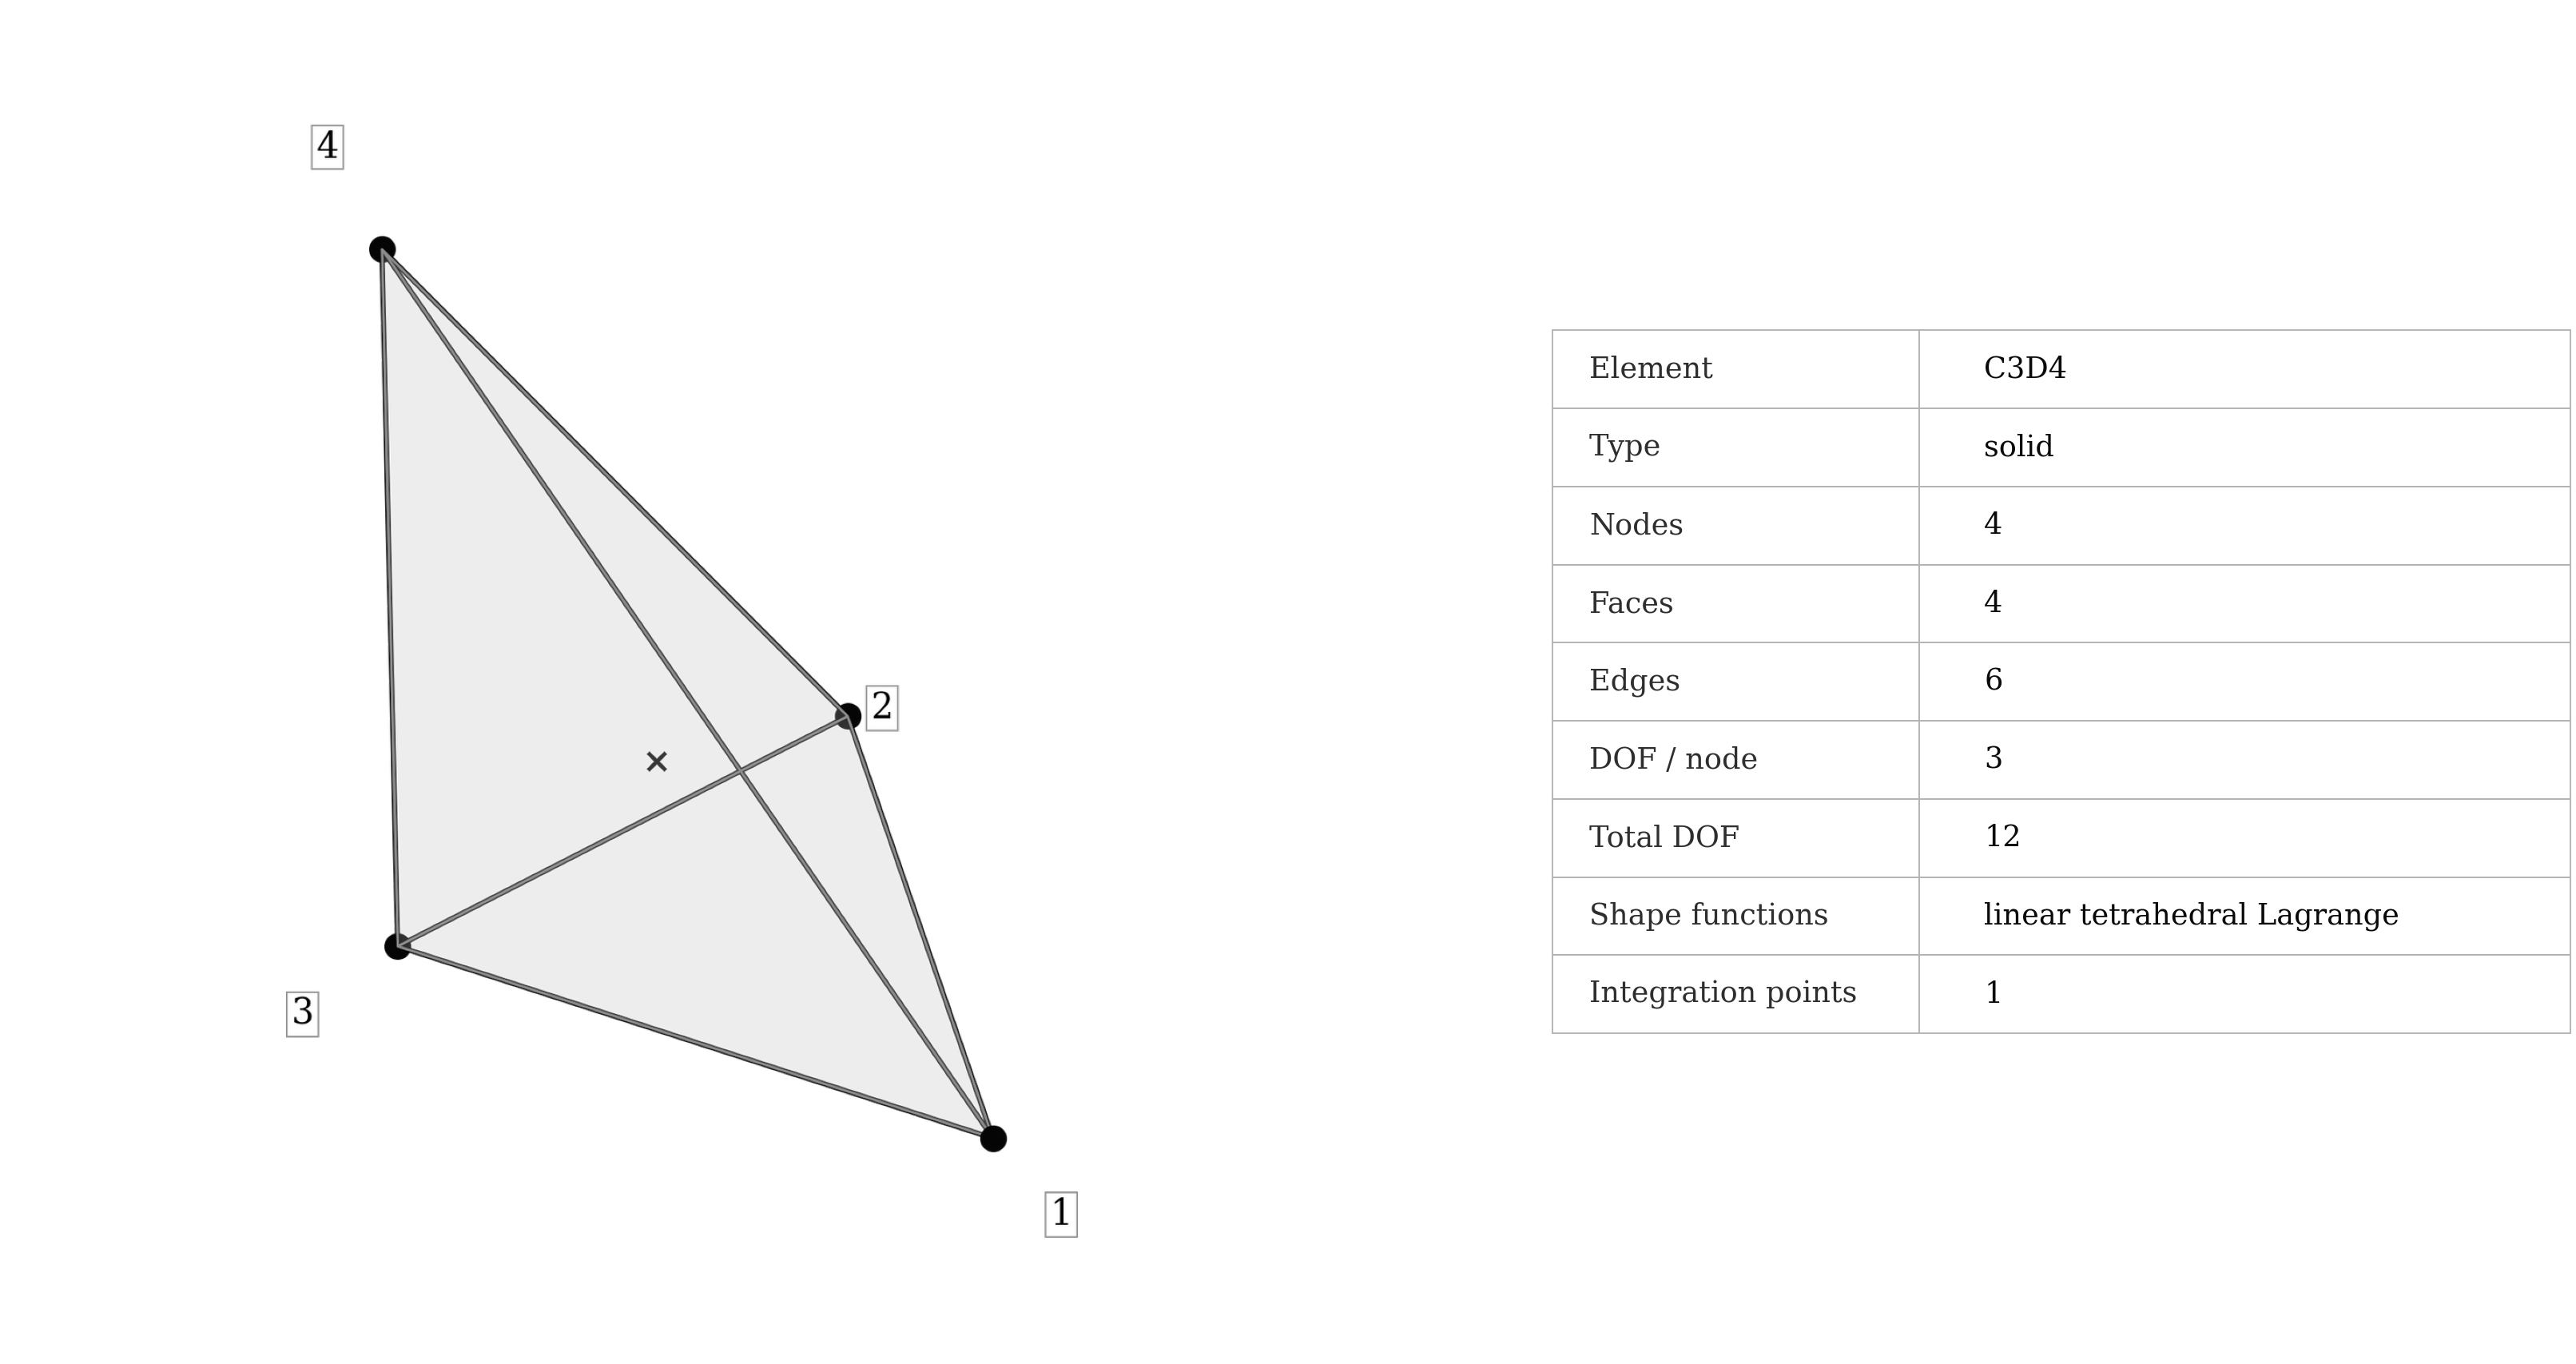
\includegraphics[width=0.78\linewidth]{pages/figures/element_schematics/c3d4_schematic.png}
    \caption{\val{C3D4} element topology and integration scheme.}
\end{figure}

\begin{syntax}
*ELEMENT, TYPE=C3D4, ELSET=<set>
<id>, <n1>, <n2>, <n3>, <n4>
\end{syntax}

\val{C3D4} is the simplest three-dimensional continuum element in FEMaster. It uses four corner nodes and linear displacement interpolation over a tetrahedral reference domain. The resulting strain field is constant within one element, which makes the element inexpensive and geometrically easy to mesh but limits the deformation and stress gradients that a single element can reproduce.

The principal advantage of \val{C3D4} is meshing flexibility. Tetrahedra can fill complex CAD volumes, narrow transitions, and irregular local details with little manual topology design. This supports early stiffness checks, coarse load-path studies, and robust automatic meshing at the cost of stress accuracy per degree of freedom.

The limitation is stiffness and stress resolution. Linear tetrahedra tend to be overly stiff in bending-dominated problems unless the mesh is fine. Since the strain state is constant in each element, stress fields can appear piecewise constant or patchy and steep gradients near holes, fillets, notches, and concentrated loads require substantial refinement.

Compared with \val{C3D4}, \val{C3D10} provides higher-order tetrahedral stress resolution in tetrahedral meshes. The sensitivity of \val{C3D4} results to refinement appears in displacements, reactions, strain energy, and averaged stresses, while a single coarse local peak is not a convergence measure.

\clearpage
\paragraph{\val{C3D5}: 5-node pyramid input}

\begin{figure}[H]
    \centering
    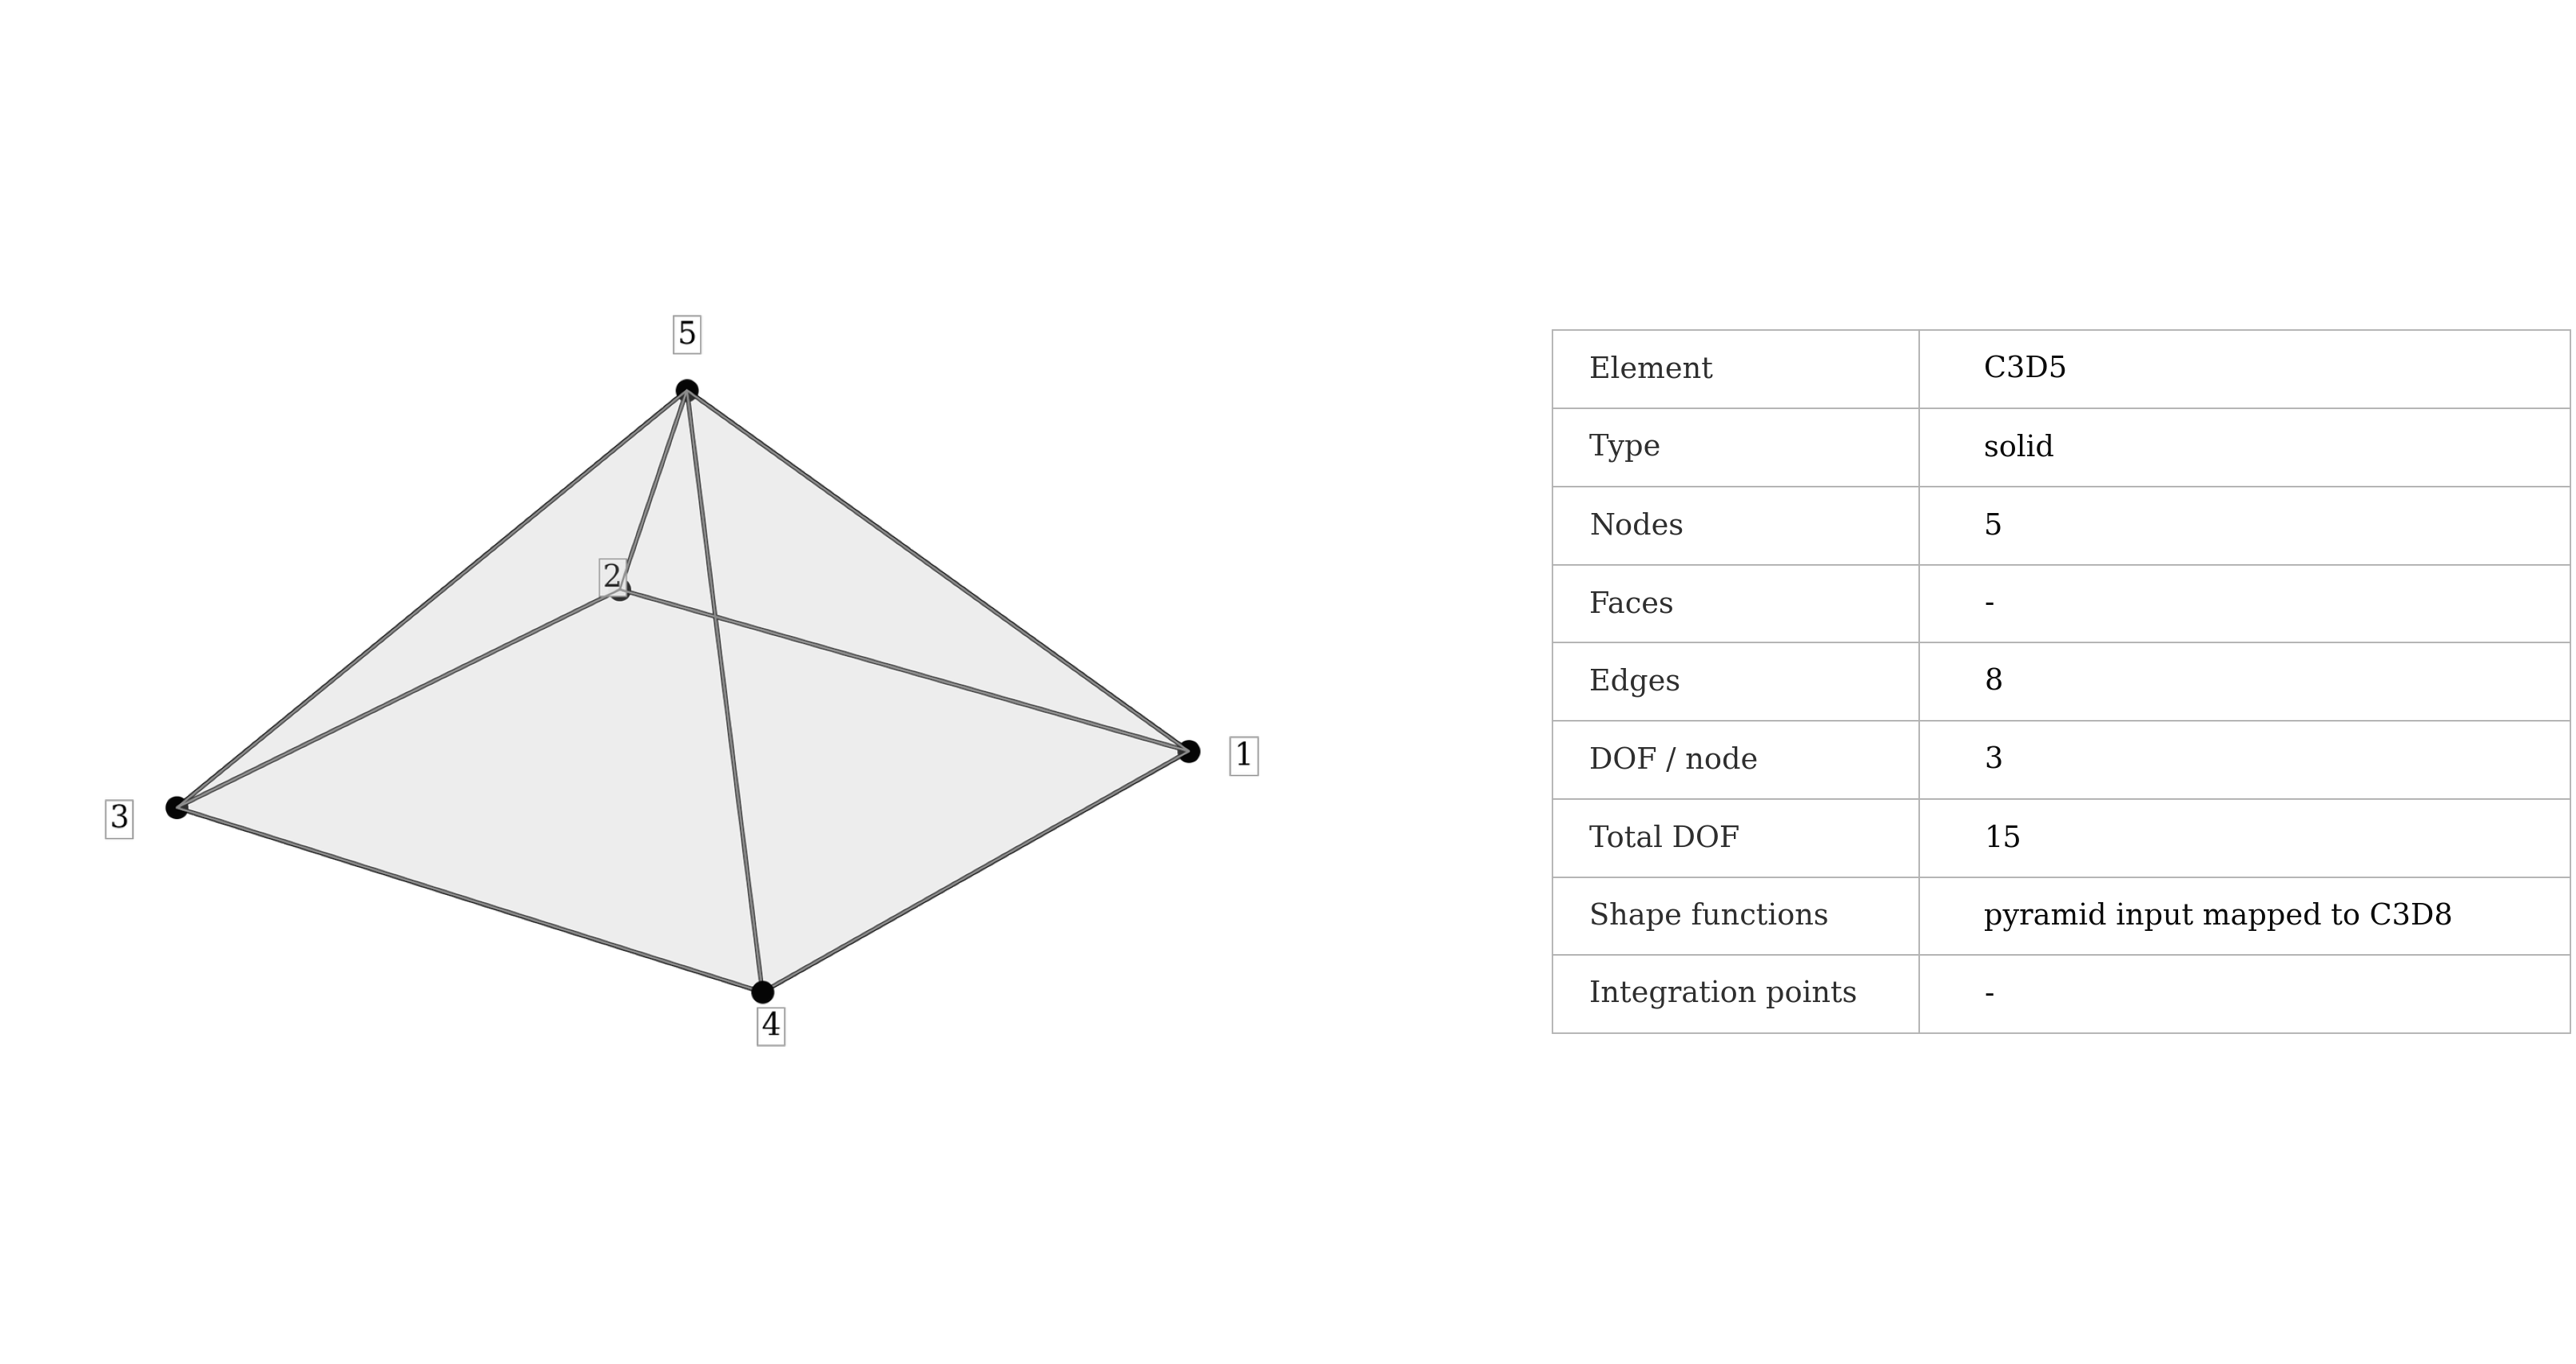
\includegraphics[width=0.78\linewidth]{pages/figures/element_schematics/c3d5_schematic.png}
    \caption{\val{C3D5} pyramid input topology.}
\end{figure}

\begin{syntax}
*ELEMENT, TYPE=C3D5, ELSET=<set>
<id>, <n1>, <n2>, <n3>, <n4>, <apex>
\end{syntax}

\val{C3D5} provides a five-node pyramid connectivity for transition meshes. FEMaster represents this input with a degenerated eight-node hexahedral topology in which the four upper hexahedral positions coincide at the pyramid apex. The user nevertheless writes the natural five-node pyramid connectivity shown above.

The element primarily acts as a transition cell between hexahedral and tetrahedral regions. In automatically generated mixed meshes, it connects a quadrilateral face to tetrahedral topology without forcing a large surrounding region to change element family.

A degenerated mapping is generally less predictable than a regular hexahedron, wedge, or tetrahedron. Flat pyramids, badly skewed bases, and apex positions close to the base plane can produce poor Jacobians and unreliable stiffness. These properties limit \val{C3D5} primarily to transition regions rather than large stress-critical volumes.

In models with many pyramids in the primary load path, reactions and global stiffness can remain plausible even when local stress quality differs significantly from an alternative regular-element mesh.

\clearpage
\paragraph{\val{C3D6}: 6-node wedge solid}

\begin{figure}[H]
    \centering
    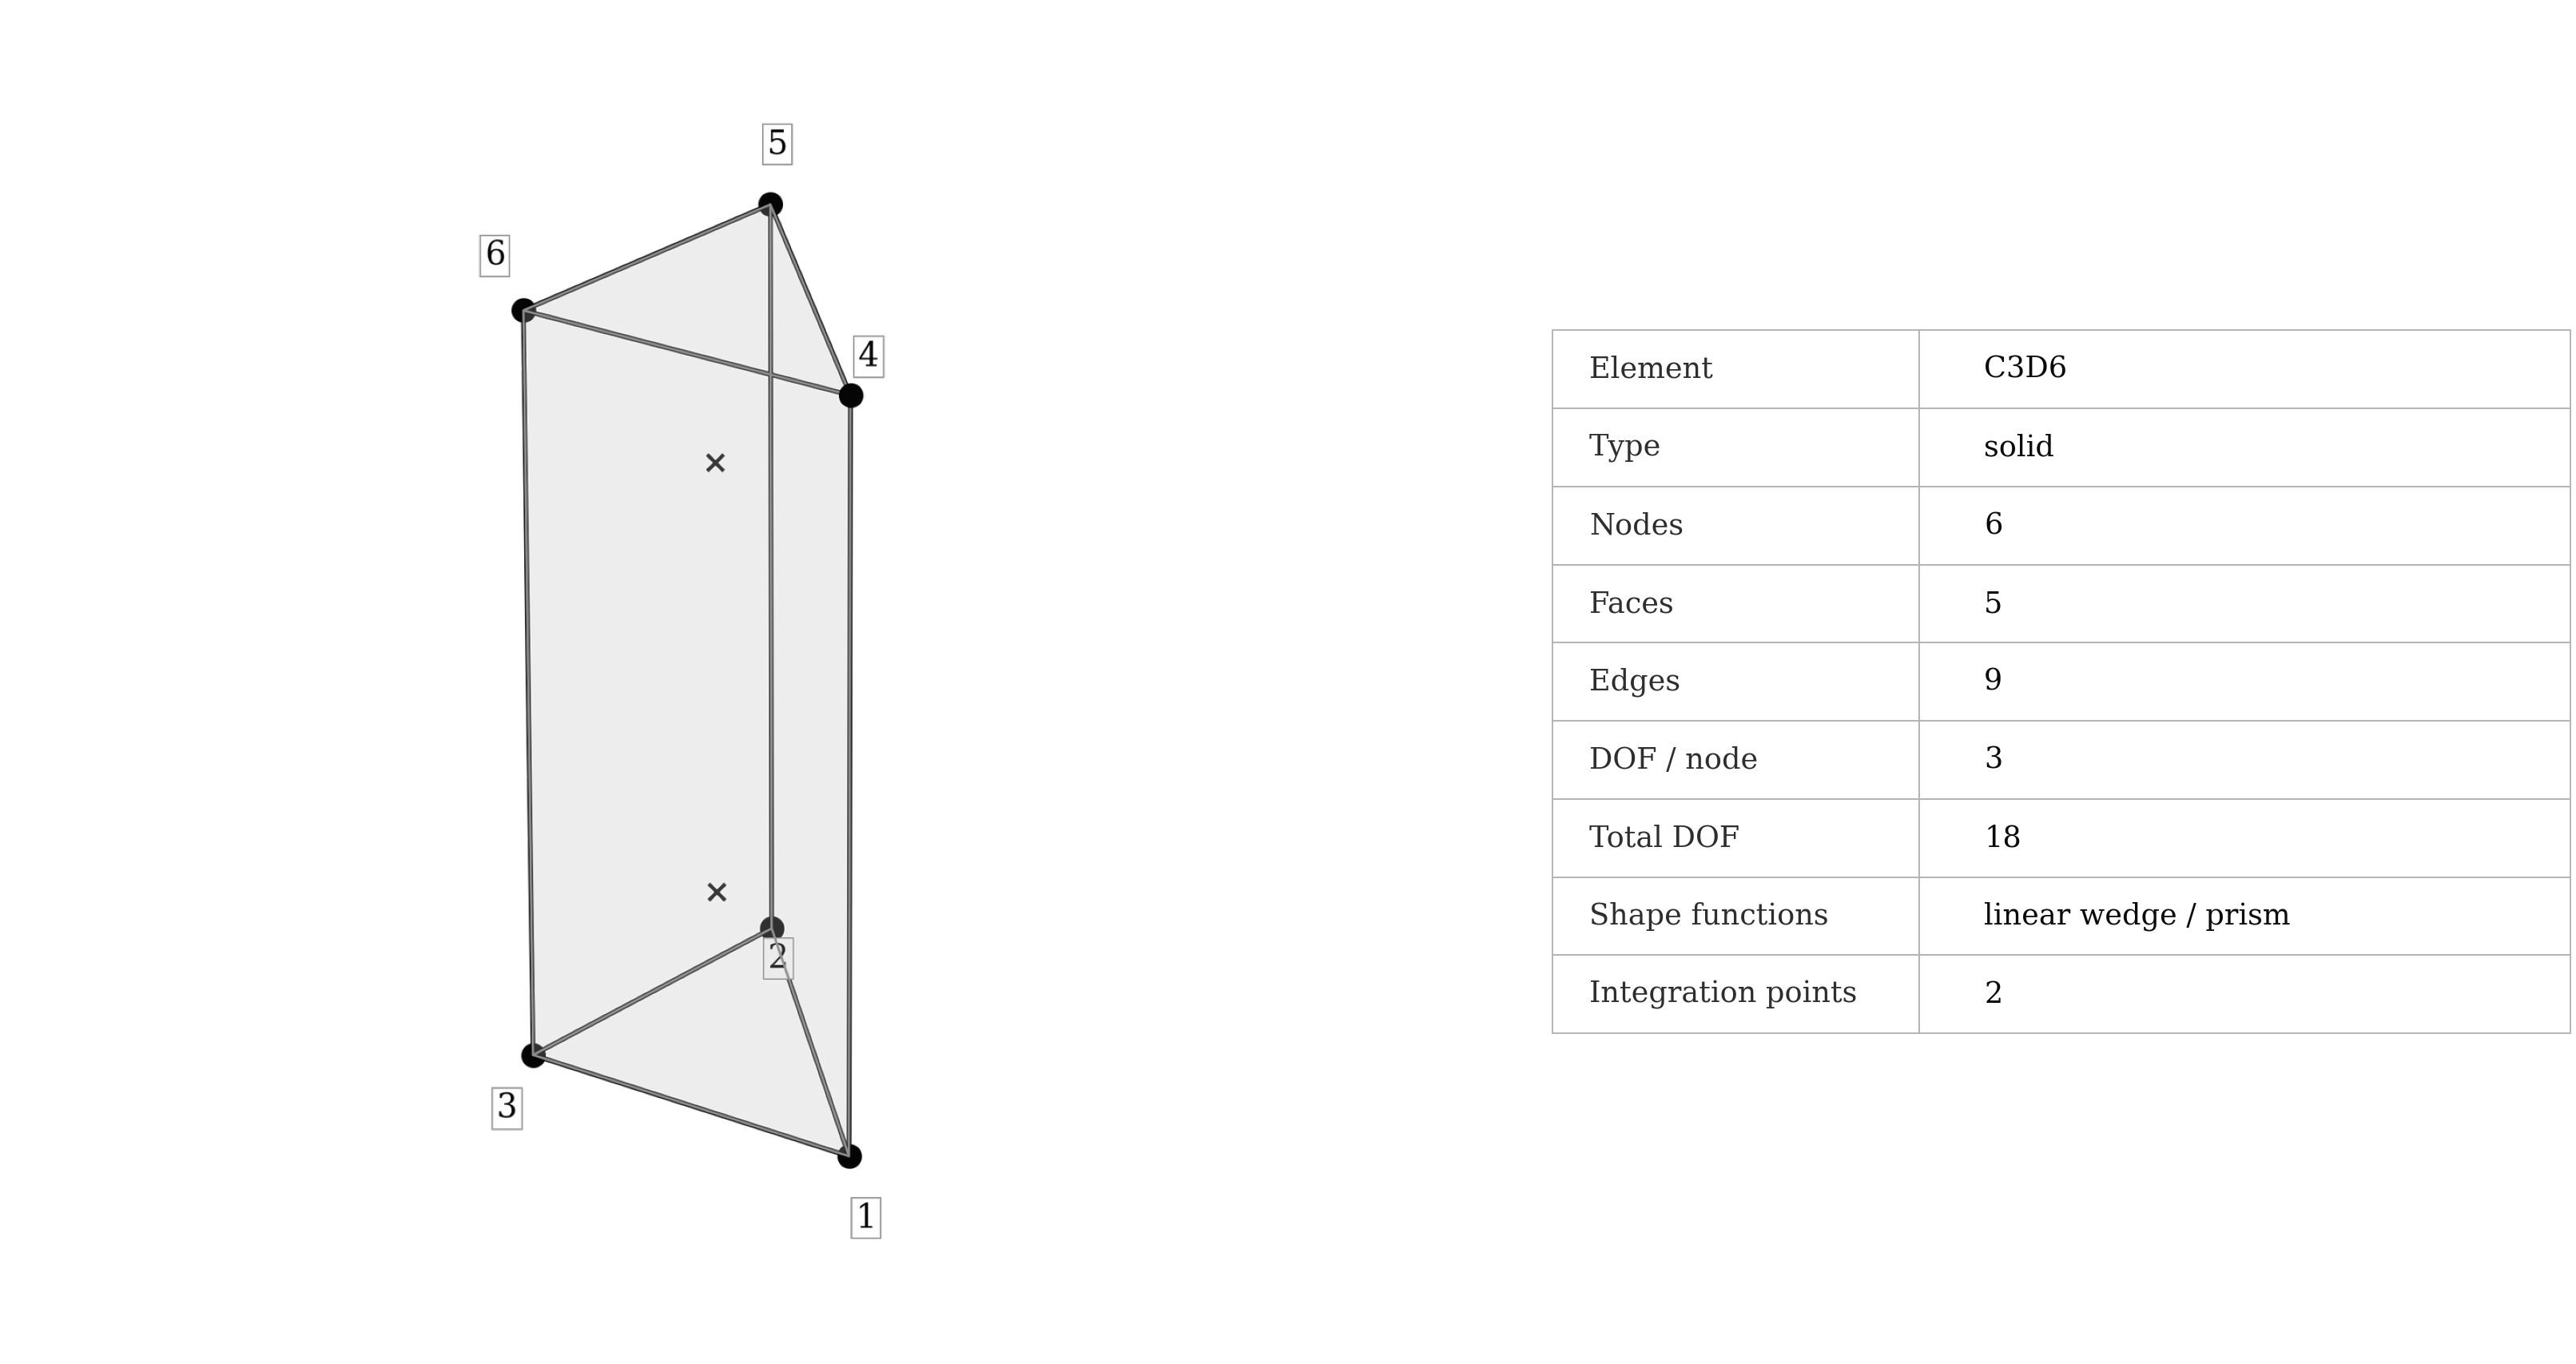
\includegraphics[width=0.78\linewidth]{pages/figures/element_schematics/c3d6_schematic.png}
    \caption{\val{C3D6} wedge element.}
\end{figure}

\begin{syntax}
*ELEMENT, TYPE=C3D6, ELSET=<set>
<id>, <n1>, <n2>, <n3>, <n4>, <n5>, <n6>
\end{syntax}

\val{C3D6} is a linear wedge or prism element. It combines triangular end faces with quadrilateral side faces and represents swept meshes, extruded triangular surface meshes, layered regions, and transitions where a purely hexahedral topology is not possible.

A wedge mesh can align naturally with a dominant through-thickness or extrusion direction. In locally layered solids and prismatic regions, its element rows can follow the physical geometry more consistently than an unstructured tetrahedral mesh.

Like other low-order elements, \val{C3D6} has limited bending and gradient resolution. One or two linear wedges through the thickness of a bending-dominated region provide limited stress recovery. Resolution increases with the number of elements in the gradient direction, while collapsed triangular faces, excessive twisting between end faces, and highly skewed side faces degrade the mapping.

\val{C3D6} matches geometries with a natural wedge topology. \val{C3D15} provides the corresponding higher-order interpolation for quadratic swept meshes.

\clearpage
\paragraph{\val{C3D8}: 8-node hexahedral solid}

\begin{figure}[H]
    \centering
    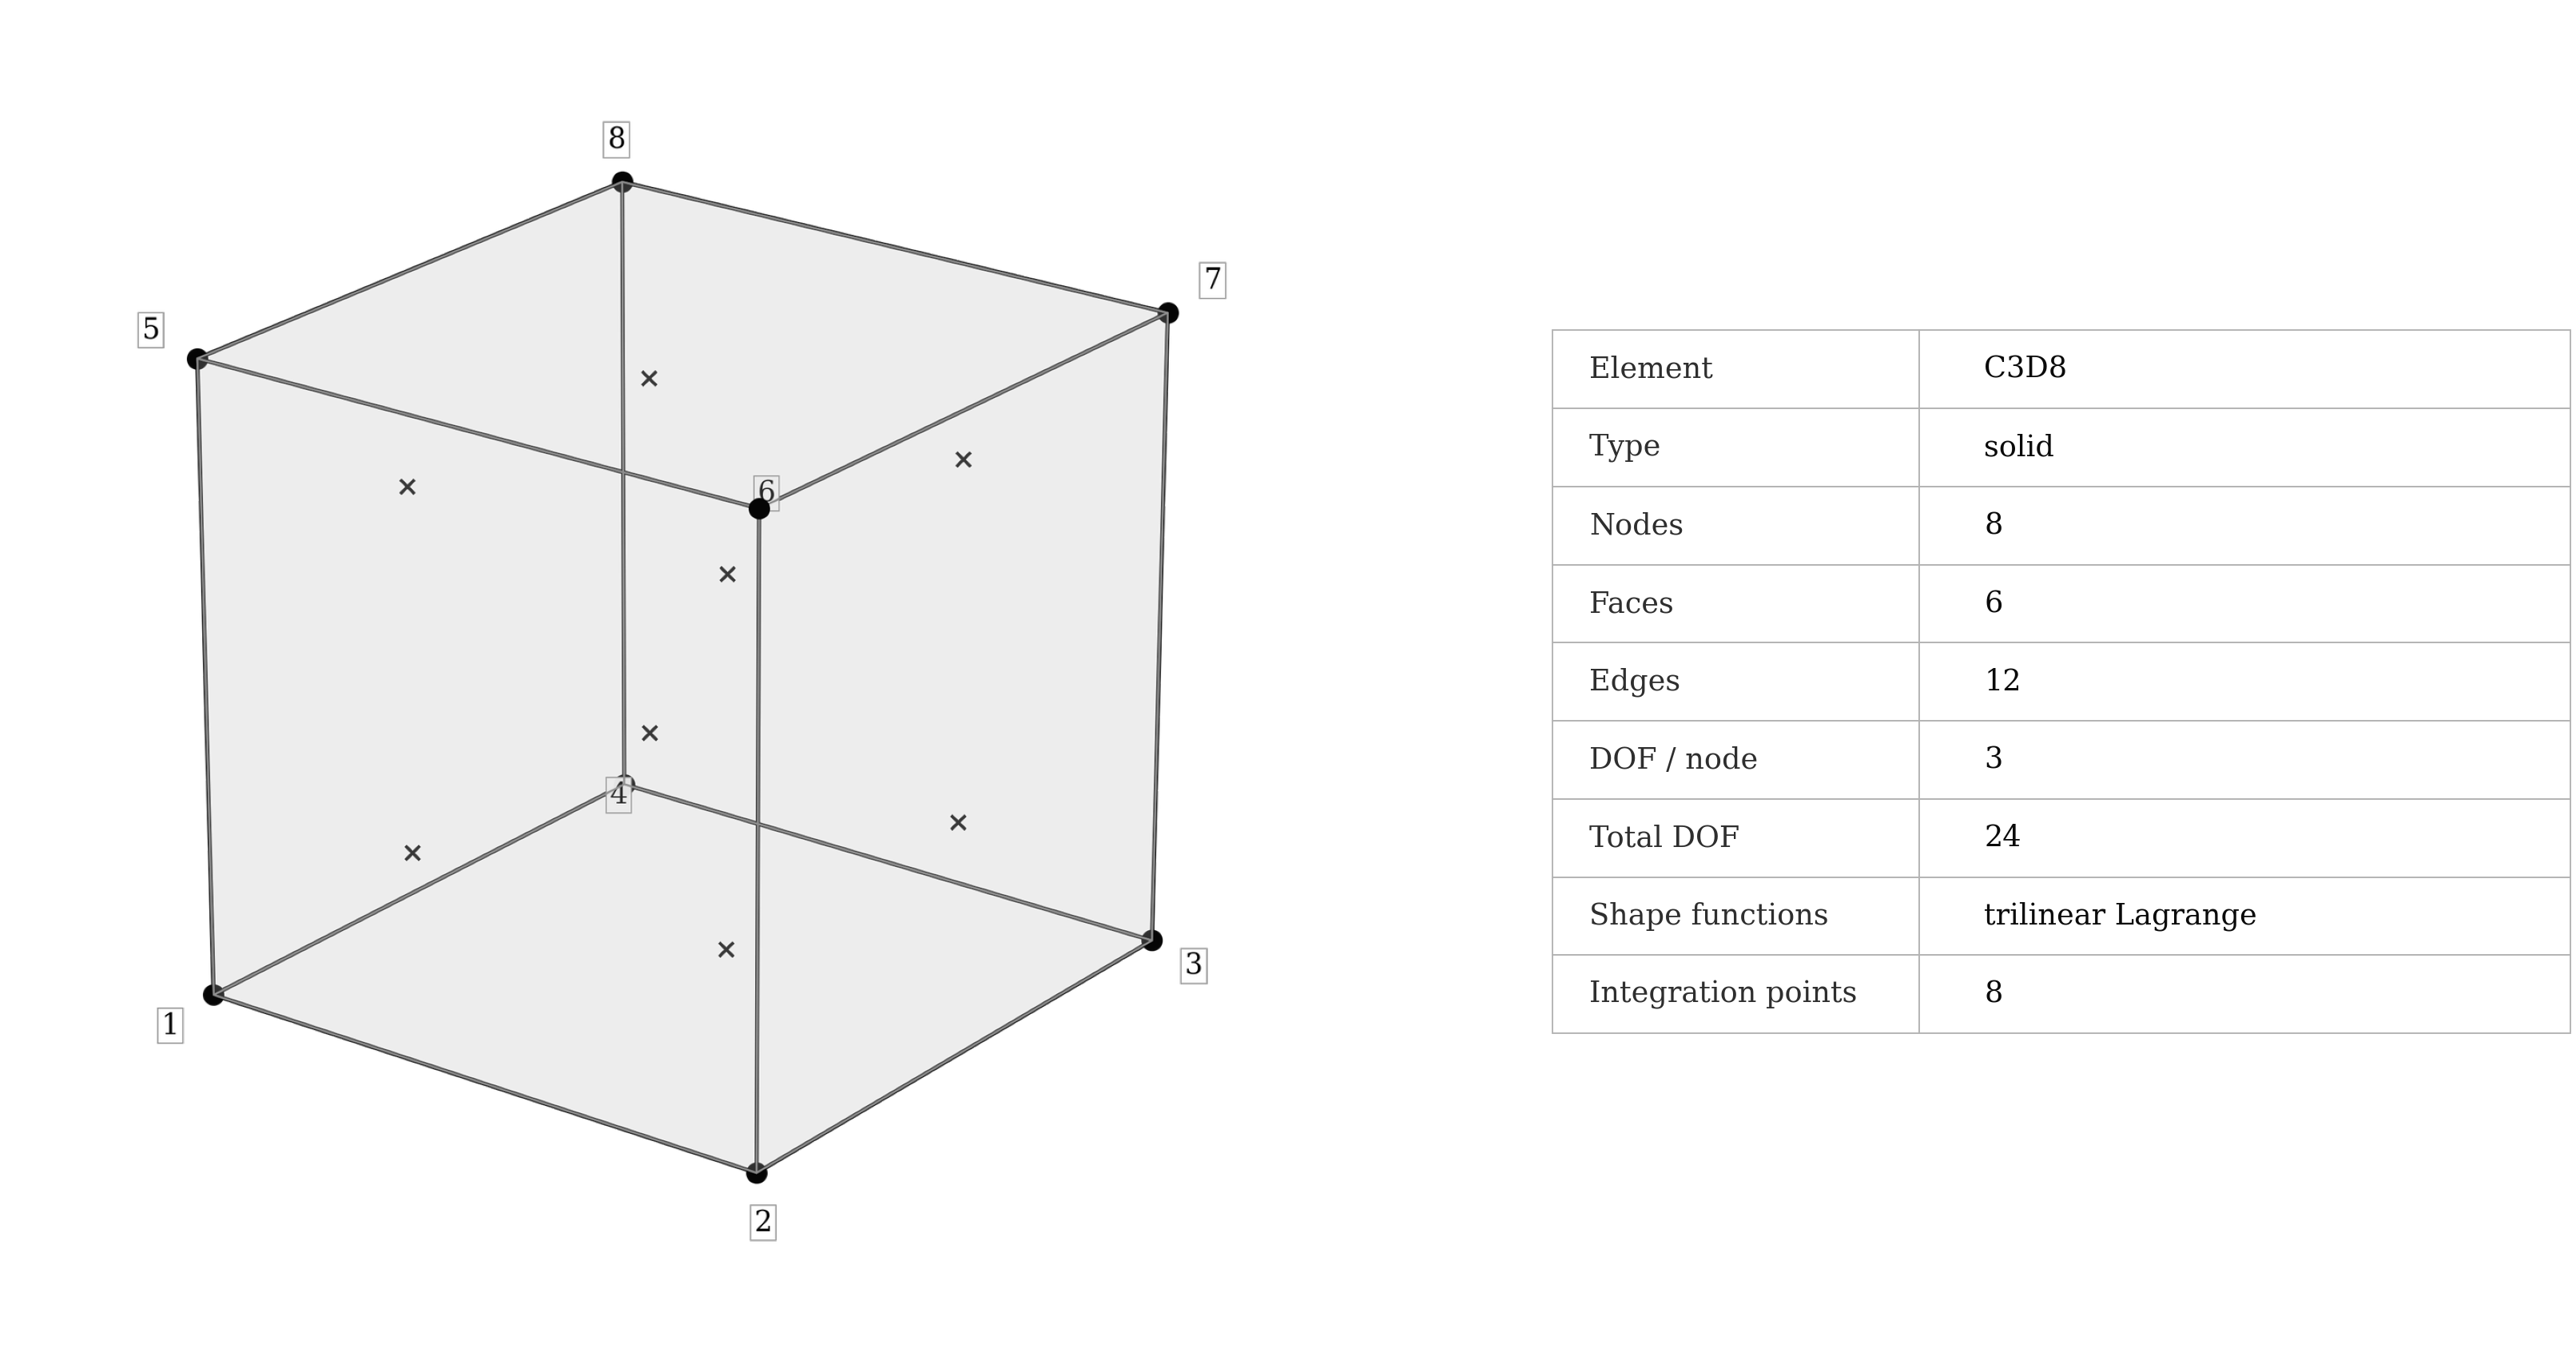
\includegraphics[width=0.82\linewidth]{pages/figures/element_schematics/c3d8_schematic.png}
    \caption{\val{C3D8} hexahedral solid element.}
\end{figure}

\begin{syntax}
*ELEMENT, TYPE=C3D8, ELSET=<set>
<id>, <n1>, <n2>, <n3>, <n4>, <n5>, <n6>, <n7>, <n8>
\end{syntax}

\val{C3D8} is the standard low-order hexahedral continuum element. It uses trilinear displacement interpolation and full integration. For regular block-like, swept, or layered meshes it is often an efficient general-purpose solid because element directions can follow geometry and material orientation naturally.

Hexahedral topology provides direct control of the number of elements through thickness and along structural load paths. A regular \val{C3D8} mesh therefore represents plates modelled with solids, bonded layers, spars, ribs, extruded components, and regions whose orthotropic material axes follow the mesh.

The element remains low order. A coarse mesh can be too stiff in bending, and straight element edges only approximate curved boundaries. Through-thickness resolution and refinement of curved or stress-critical geometry directly control the corresponding bending-stress and geometry errors.

Warping, skew, negative Jacobians, and extreme aspect ratios can remove the numerical advantages of the hexahedral topology. A clean quadratic tetrahedral mesh can provide a more accurate mapping than a badly distorted hexahedral mesh; topology alone does not determine mesh quality.

\clearpage
\paragraph{\val{C3D8I}: incompatible-mode 8-node hexahedral solid}

\begin{figure}[H]
    \centering
    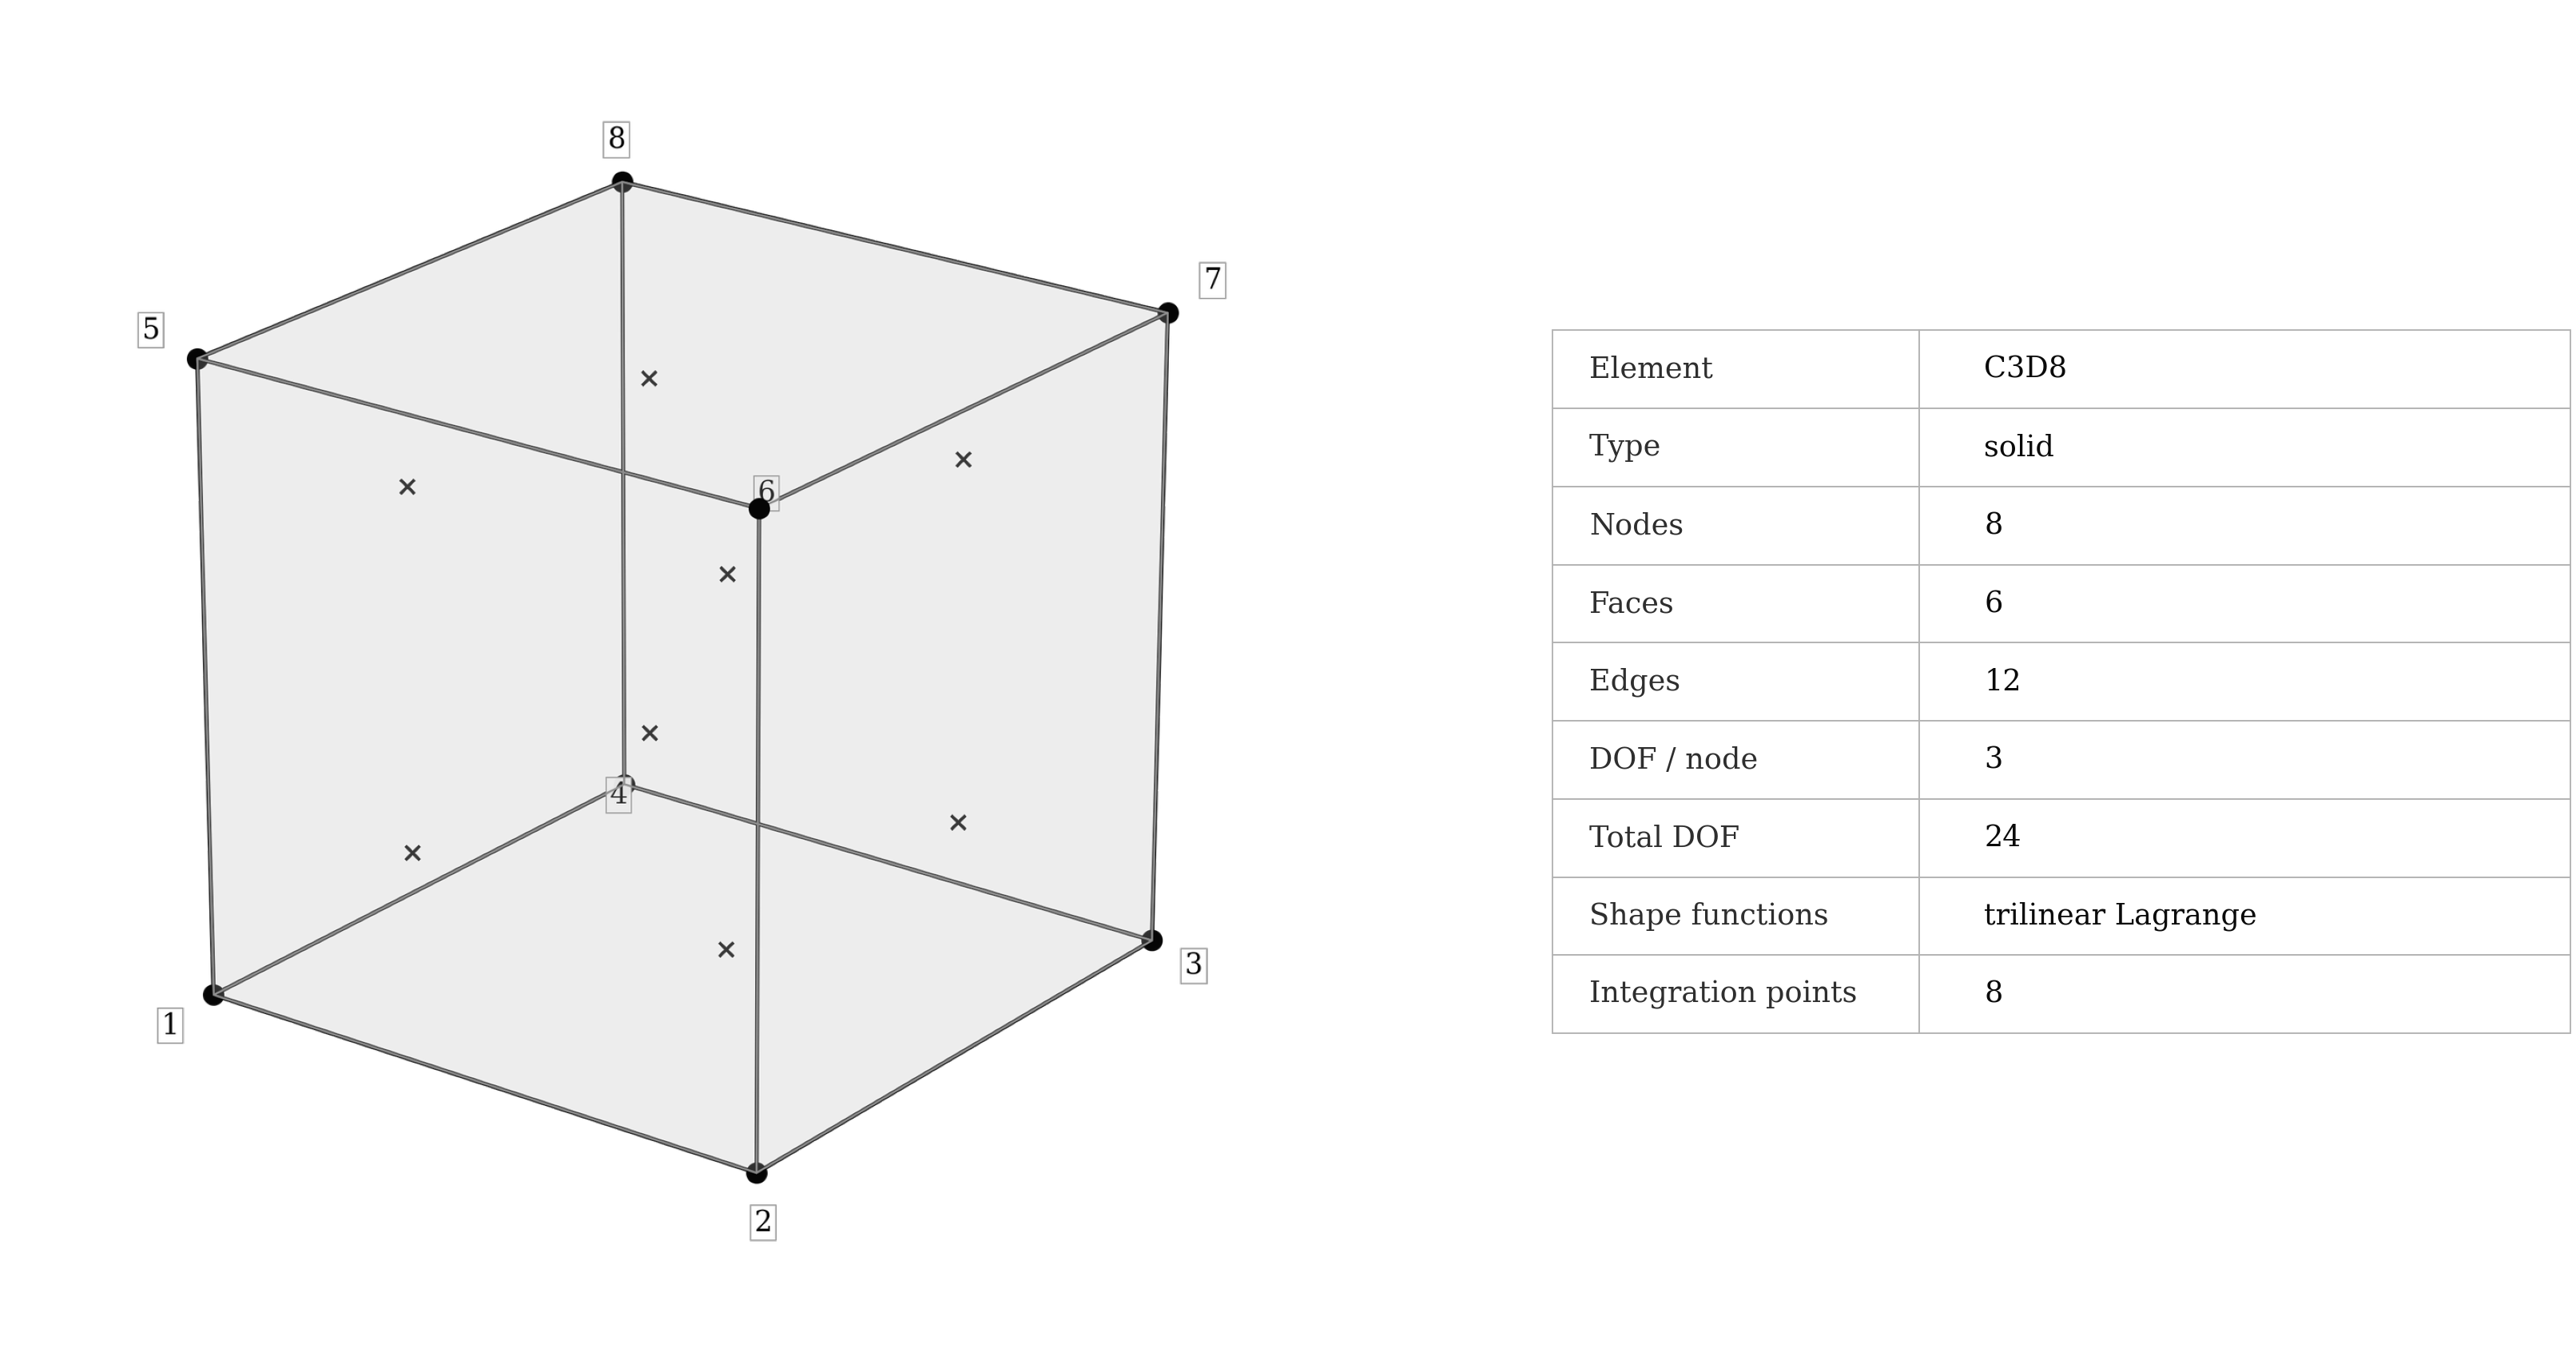
\includegraphics[width=0.82\linewidth]{pages/figures/element_schematics/c3d8_schematic.png}
    \caption{\val{C3D8I} topology; the eight external nodes are identical to \val{C3D8}.}
\end{figure}

\begin{syntax}
*ELEMENT, TYPE=C3D8I, ELSET=<set>
<id>, <n1>, <n2>, <n3>, <n4>, <n5>, <n6>, <n7>, <n8>
\end{syntax}

\val{C3D8I} uses the same trilinear eight-node geometry and the same full
\(2\times2\times2\) integration rule as \val{C3D8}. Its compatible displacement
field is augmented by 13 element-local enhanced modes. Nine principal
vector-valued modes improve bending behaviour by removing parasitic constraints
of the low-order compatible interpolation; four additional volumetric modes
improve the response in nearly incompressible states.

The 13 enhanced parameters are internal to each element. FEMaster solves their
local stationarity equations and statically condenses them, so a \val{C3D8I}
still contributes only the 24 translational nodal degrees of freedom of an
ordinary eight-node solid to the global system. Unlike \val{C3D8R}, the element
does not rely on reduced integration or hourglass stabilization.

For geometrically nonlinear analysis the enhanced parameters are solved by a
local Newton iteration at every element evaluation and the complete material and
geometric tangent blocks are condensed by a Schur complement. The finite-strain
kinematics use a right multiplicative enhancement
\[
\bar{\mathbf F}
=
\mathbf F_c
\left(
\mathbf I + \sum_m \alpha_m \mathbf H_m
\right).
\]
The enhanced tensors therefore remain in the reference configuration. A
superposed spatial rigid rotation maps
\(\bar{\mathbf F}\rightarrow\mathbf Q\bar{\mathbf F}\), so the enhanced
mode space and condensed response remain objective.

\val{C3D8I} is intended primarily for low-order hexahedral meshes in which
bending or near-incompressibility makes a standard \val{C3D8} unnecessarily
stiff. It remains a trilinear geometry mapping and is still sensitive to severe
warping and skew. The incompatible modes improve the kinematics; they do not turn
a poor eight-node geometry into a higher-order element.

\clearpage
\paragraph{\val{C3D8R}: reduced-integration 8-node hexahedral solid}

\begin{figure}[H]
    \centering
    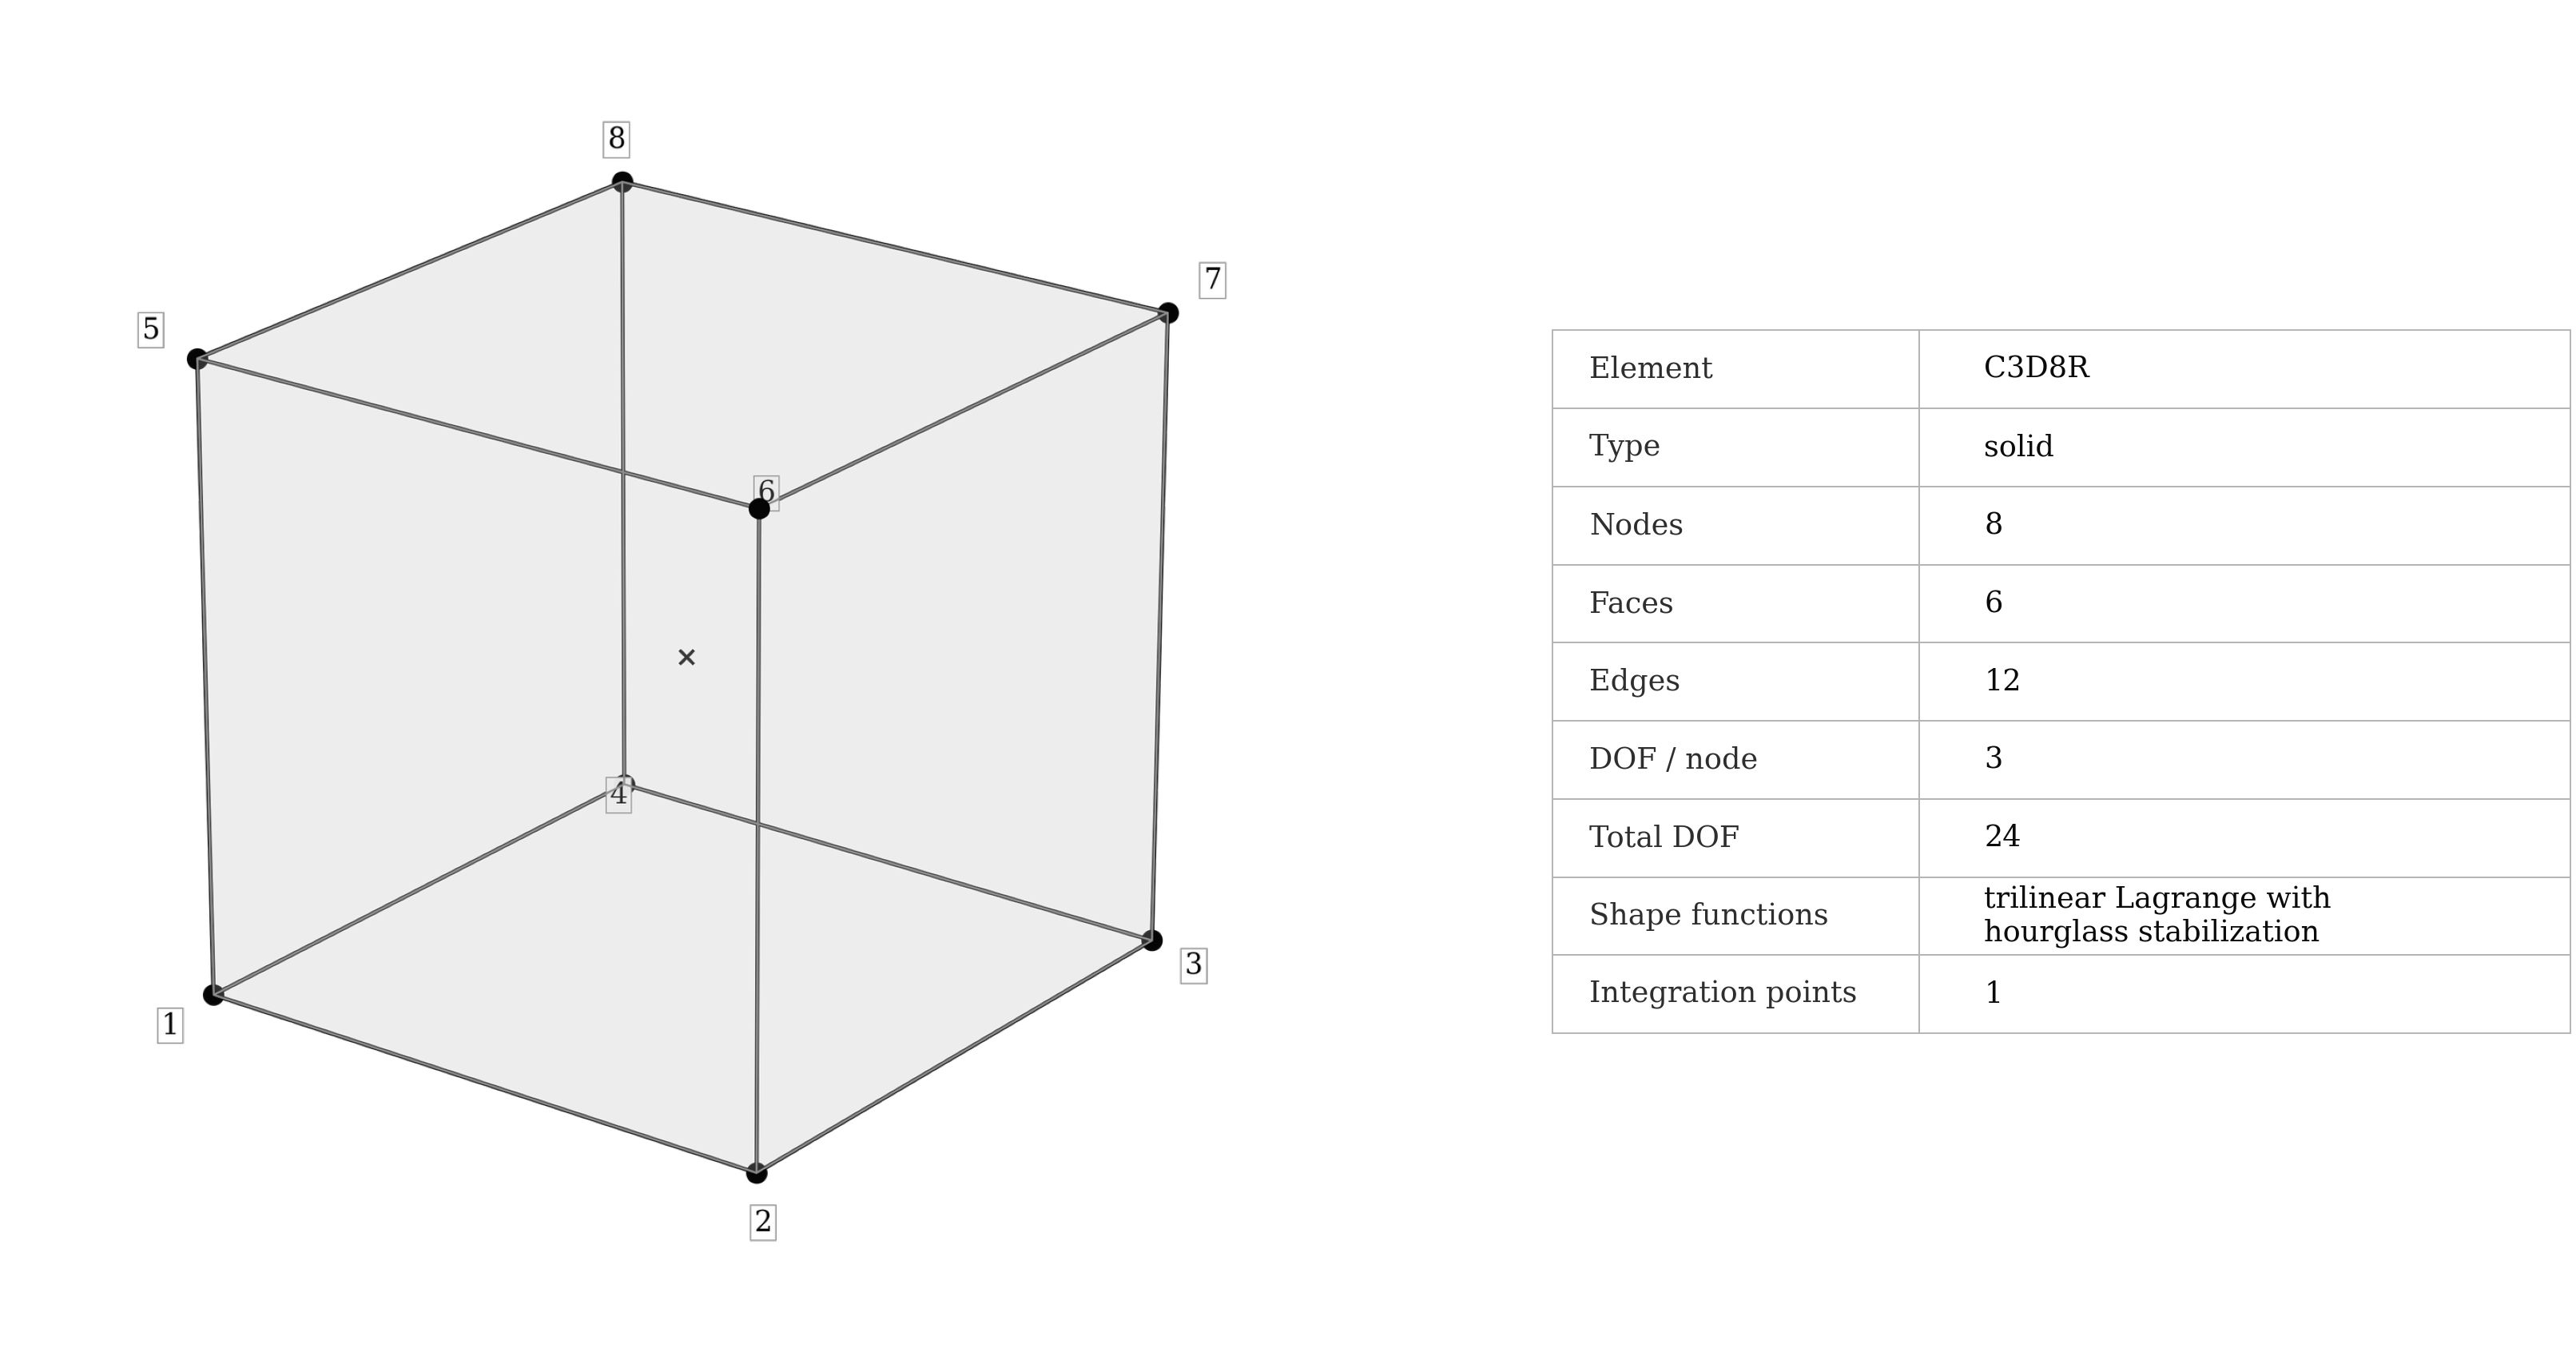
\includegraphics[width=0.82\linewidth]{pages/figures/element_schematics/c3d8r_schematic.png}
    \caption{\val{C3D8R} reduced-integration hexahedral solid element.}
\end{figure}

\begin{syntax}
*ELEMENT, TYPE=C3D8R, ELSET=<set>
<id>, <n1>, <n2>, <n3>, <n4>, <n5>, <n6>, <n7>, <n8>
\end{syntax}

\val{C3D8R} uses the same eight-node topology as \val{C3D8} but evaluates the continuum contribution with one integration point at the element centre. Reduced integration lowers assembly cost and avoids some of the excessive stiffness that a fully integrated low-order hexahedron can exhibit in bending-dominated states.

One-point integration also introduces zero-energy hourglass deformation modes. FEMaster therefore adds hourglass stabilization. The primitive scalar hourglass patterns are based on the four non-affine modes
\[
\gamma_1=s\,t,\qquad
\gamma_2=t\,r,\qquad
\gamma_3=r\,s,\qquad
\gamma_4=r\,s\,t.
\]
These modes are projected so that affine displacement fields are not penalized. The stabilization scale is based on the element reference volume, the reference geometry gradients, and an effective shear stiffness derived from the constitutive tangent. The default dimensionless hourglass coefficient is \(\alpha=0.005\).

Newton convergence alone does not characterize \val{C3D8R}; the deformation pattern and stabilization sensitivity are independent numerical properties. A coarse or badly distorted mesh can converge while exhibiting nonphysical hourglass deformation. Comparison with \val{C3D8} and mesh refinement expose response components associated with hourglass-sensitive deformation.

Severe finite rotations and highly distorted elements increase sensitivity to reduced-integration stabilization. Relative to \val{C3D8}, \val{C3D8R} exchanges lower integration cost and locking tendency for dependence on hourglass control.

\clearpage
\paragraph{\val{C3D10}: 10-node quadratic tetrahedral solid}

\begin{figure}[H]
    \centering
    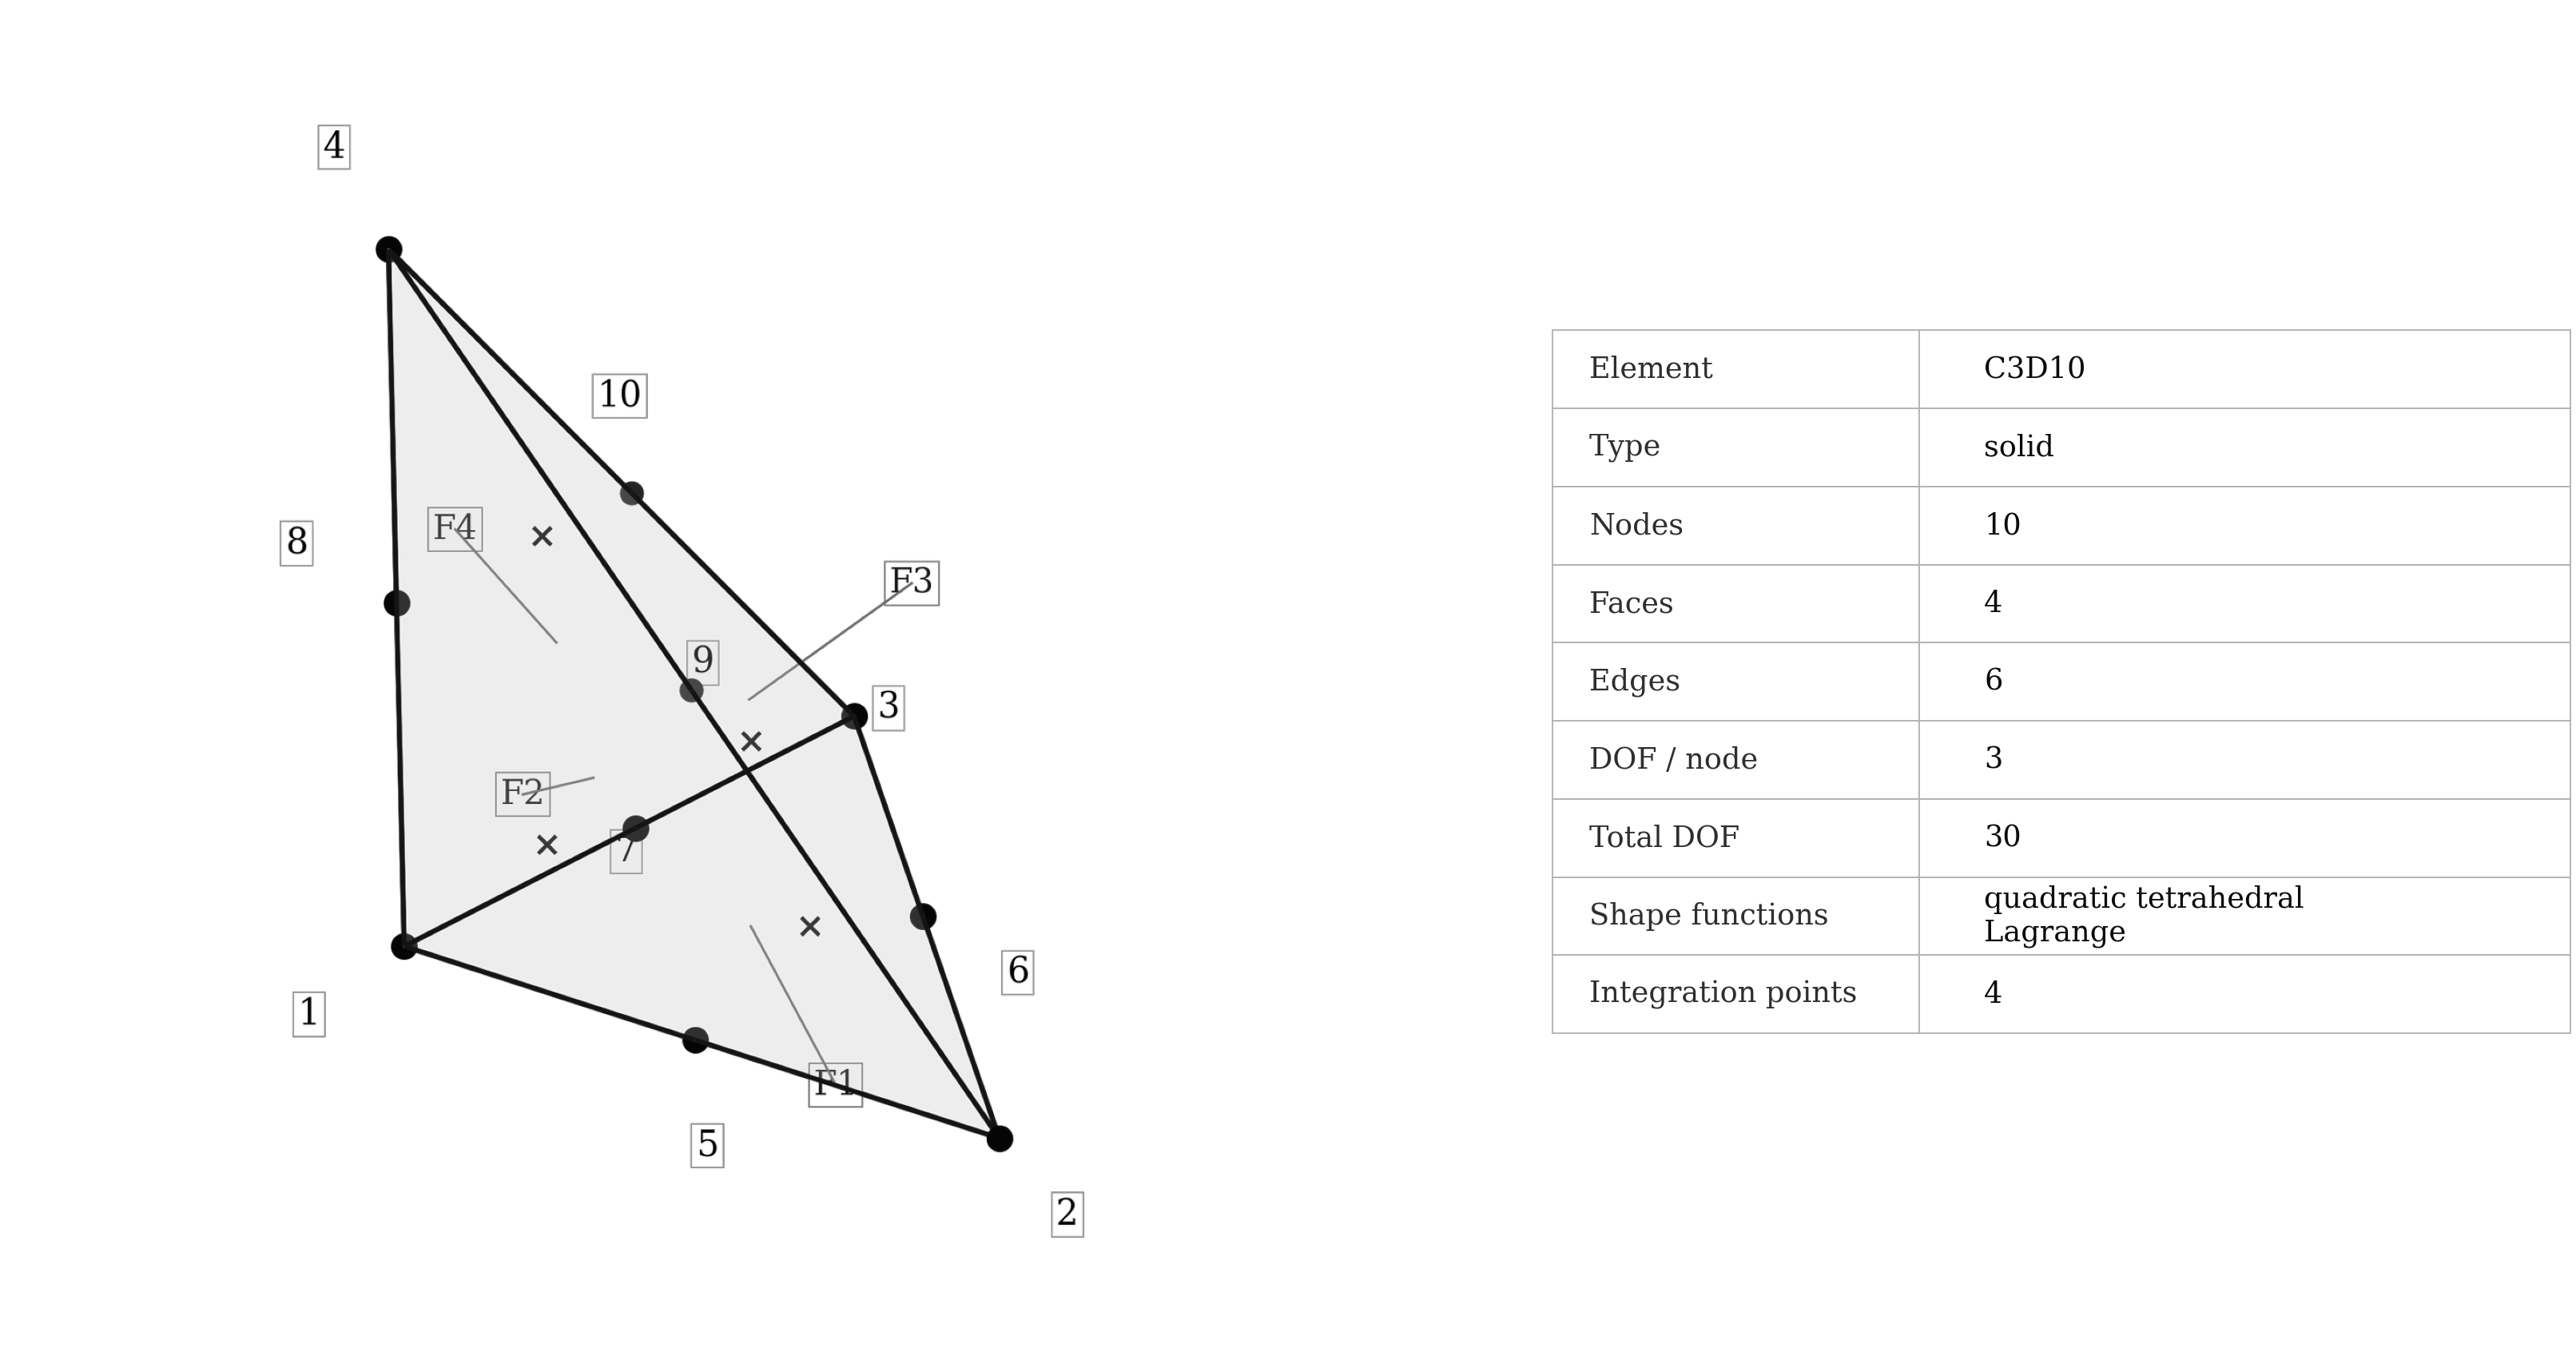
\includegraphics[width=0.80\linewidth]{pages/figures/element_schematics/c3d10_schematic.png}
    \caption{\val{C3D10} quadratic tetrahedral element.}
\end{figure}

\begin{syntax}
*ELEMENT, TYPE=C3D10, ELSET=<set>
<id>, <n1>, <n2>, <n3>, <n4>, <n5>, <n6>, <n7>, <n8>, <n9>, <n10>
\end{syntax}

\val{C3D10} is the quadratic tetrahedral solid. Six midside nodes augment the four corner nodes and allow quadratic displacement interpolation. Compared with \val{C3D4}, the element can represent curved deformation, bending, and stress gradients far more efficiently.

For automatic tetrahedral meshing, \val{C3D10} retains the geometric flexibility of tetrahedra while reducing the excessive stiffness and piecewise-constant strain behaviour associated with linear tetrahedra.

The quadratic geometry mapping also represents curved boundaries more accurately when midside nodes follow the CAD geometry. Badly displaced midside nodes can create a distorted mapping even if the corner tetrahedron appears acceptable.

The element costs more per cell than \val{C3D4}, but substantially fewer cells may be required for comparable displacement and stress accuracy. Refinement is still required near singularities, sharp re-entrant corners, and concentrated loads where no polynomial element can make a mathematical singularity disappear.

\clearpage
\paragraph{\val{C3D13}: 13-node quadratic pyramid solid}

\begin{figure}[H]
    \centering
    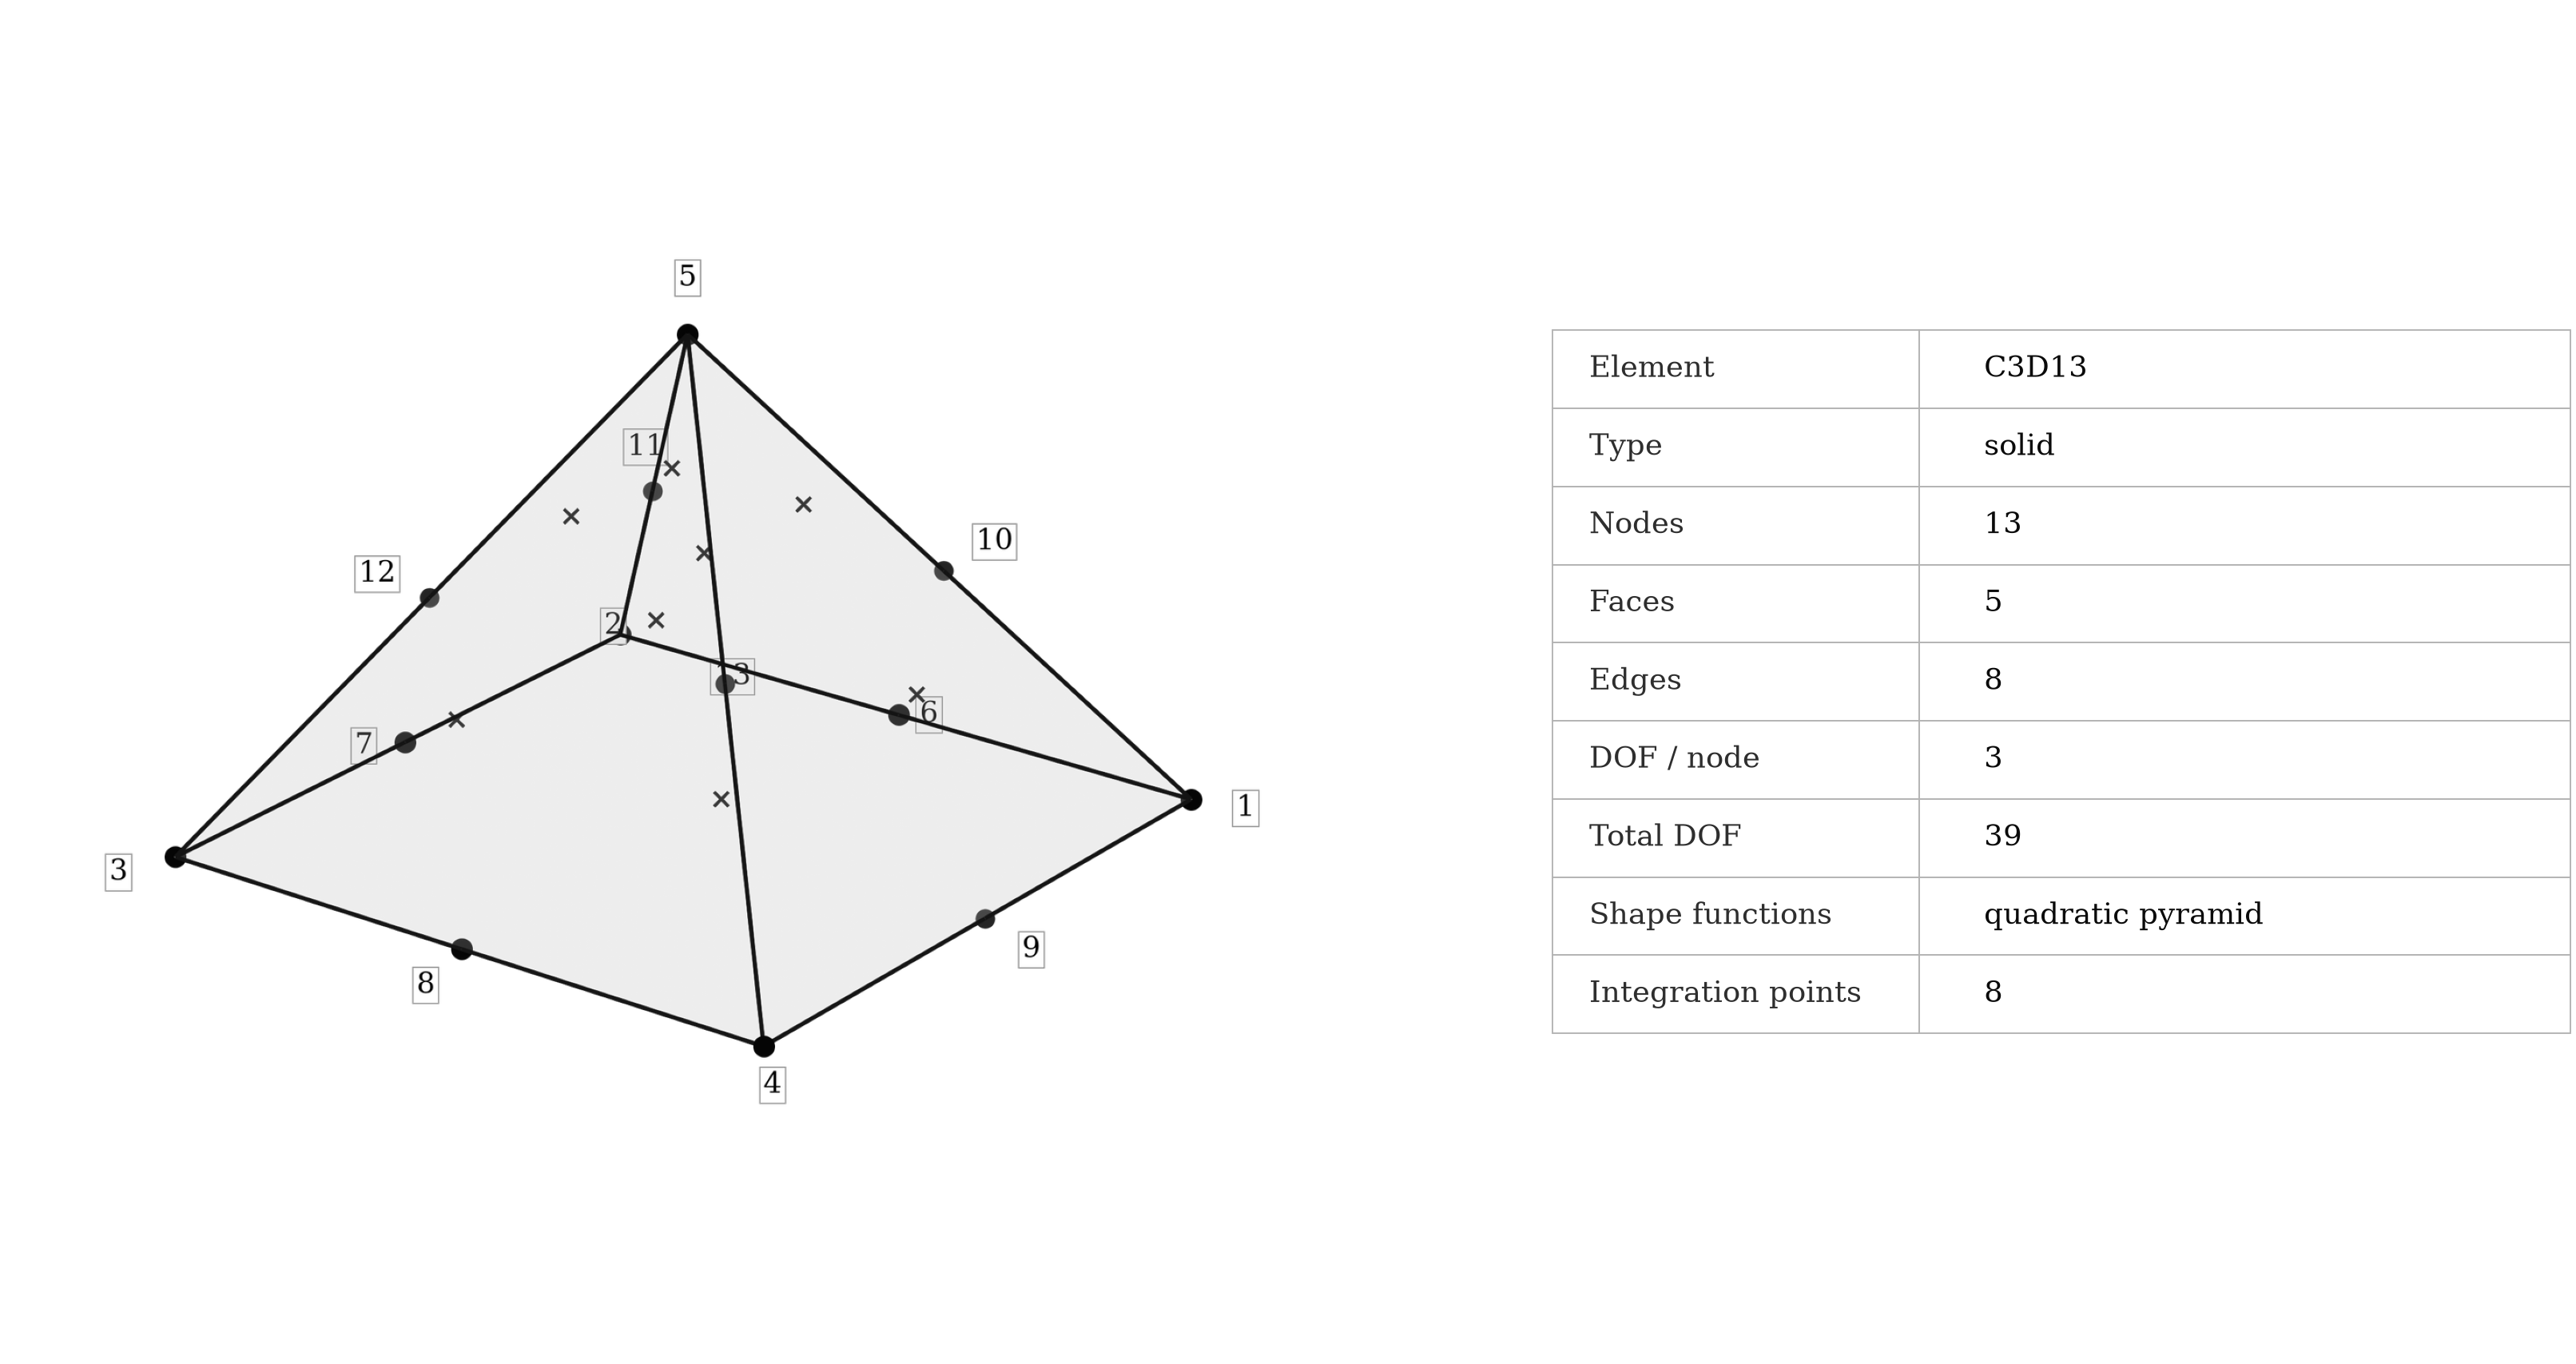
\includegraphics[width=0.78\linewidth]{pages/figures/element_schematics/c3d13_schematic.png}
    \caption{\val{C3D13} quadratic pyramid topology and integration scheme.}
\end{figure}

\begin{syntax}
*ELEMENT, TYPE=C3D13, ELSET=<set>
<id>, <n1>, <n2>, <n3>, <n4>, <n5>, <n6>, <n7>, <n8>, <n9>, <n10>, <n11>, <n12>, <n13>
\end{syntax}

\val{C3D13} is a thirteen-node quadratic pyramid element with rational
shape functions in the natural pyramid coordinates. Nodes 1--4 define
the quadrilateral base and node 5 the apex. Nodes 6--9 lie on the four
base edges, while nodes 10--13 lie between the base corners and the
apex. The rational interpolation accommodates the collapsed pyramid
geometry and provides a higher-order displacement description than
the five-node \val{C3D5} transition element.

A pyramid is useful where a quadrilateral-faced hexahedral mesh must
transition to a region containing tetrahedral cells. Compared with
\val{C3D5}, the midside nodes can represent curved edges and varying
deformation fields more accurately, provided their positions are
consistent with the intended physical geometry. Strongly distorted
pyramids or poor apex placement can still result in inaccurate
Jacobians, stiffness, and stress recovery.

The element uses the \val{DOMAIN_ISO_PYRAMID} quadrature with
\val{ORDER_QUARTIC} (27 integration points) and provides five
outward-oriented quadratic faces for surface definitions: an
eight-node quadrilateral base (\val{S1}) and four six-node
triangular sides (\val{S2}--\val{S5}). Recovered stress and strain
values are extrapolated from the constitutive integration points.
As for other quadratic solids, local stresses should be assessed
through mesh refinement rather than a single extrapolated nodal peak.

\clearpage
\paragraph{\val{C3D15}: 15-node quadratic wedge solid}

\begin{figure}[H]
    \centering
    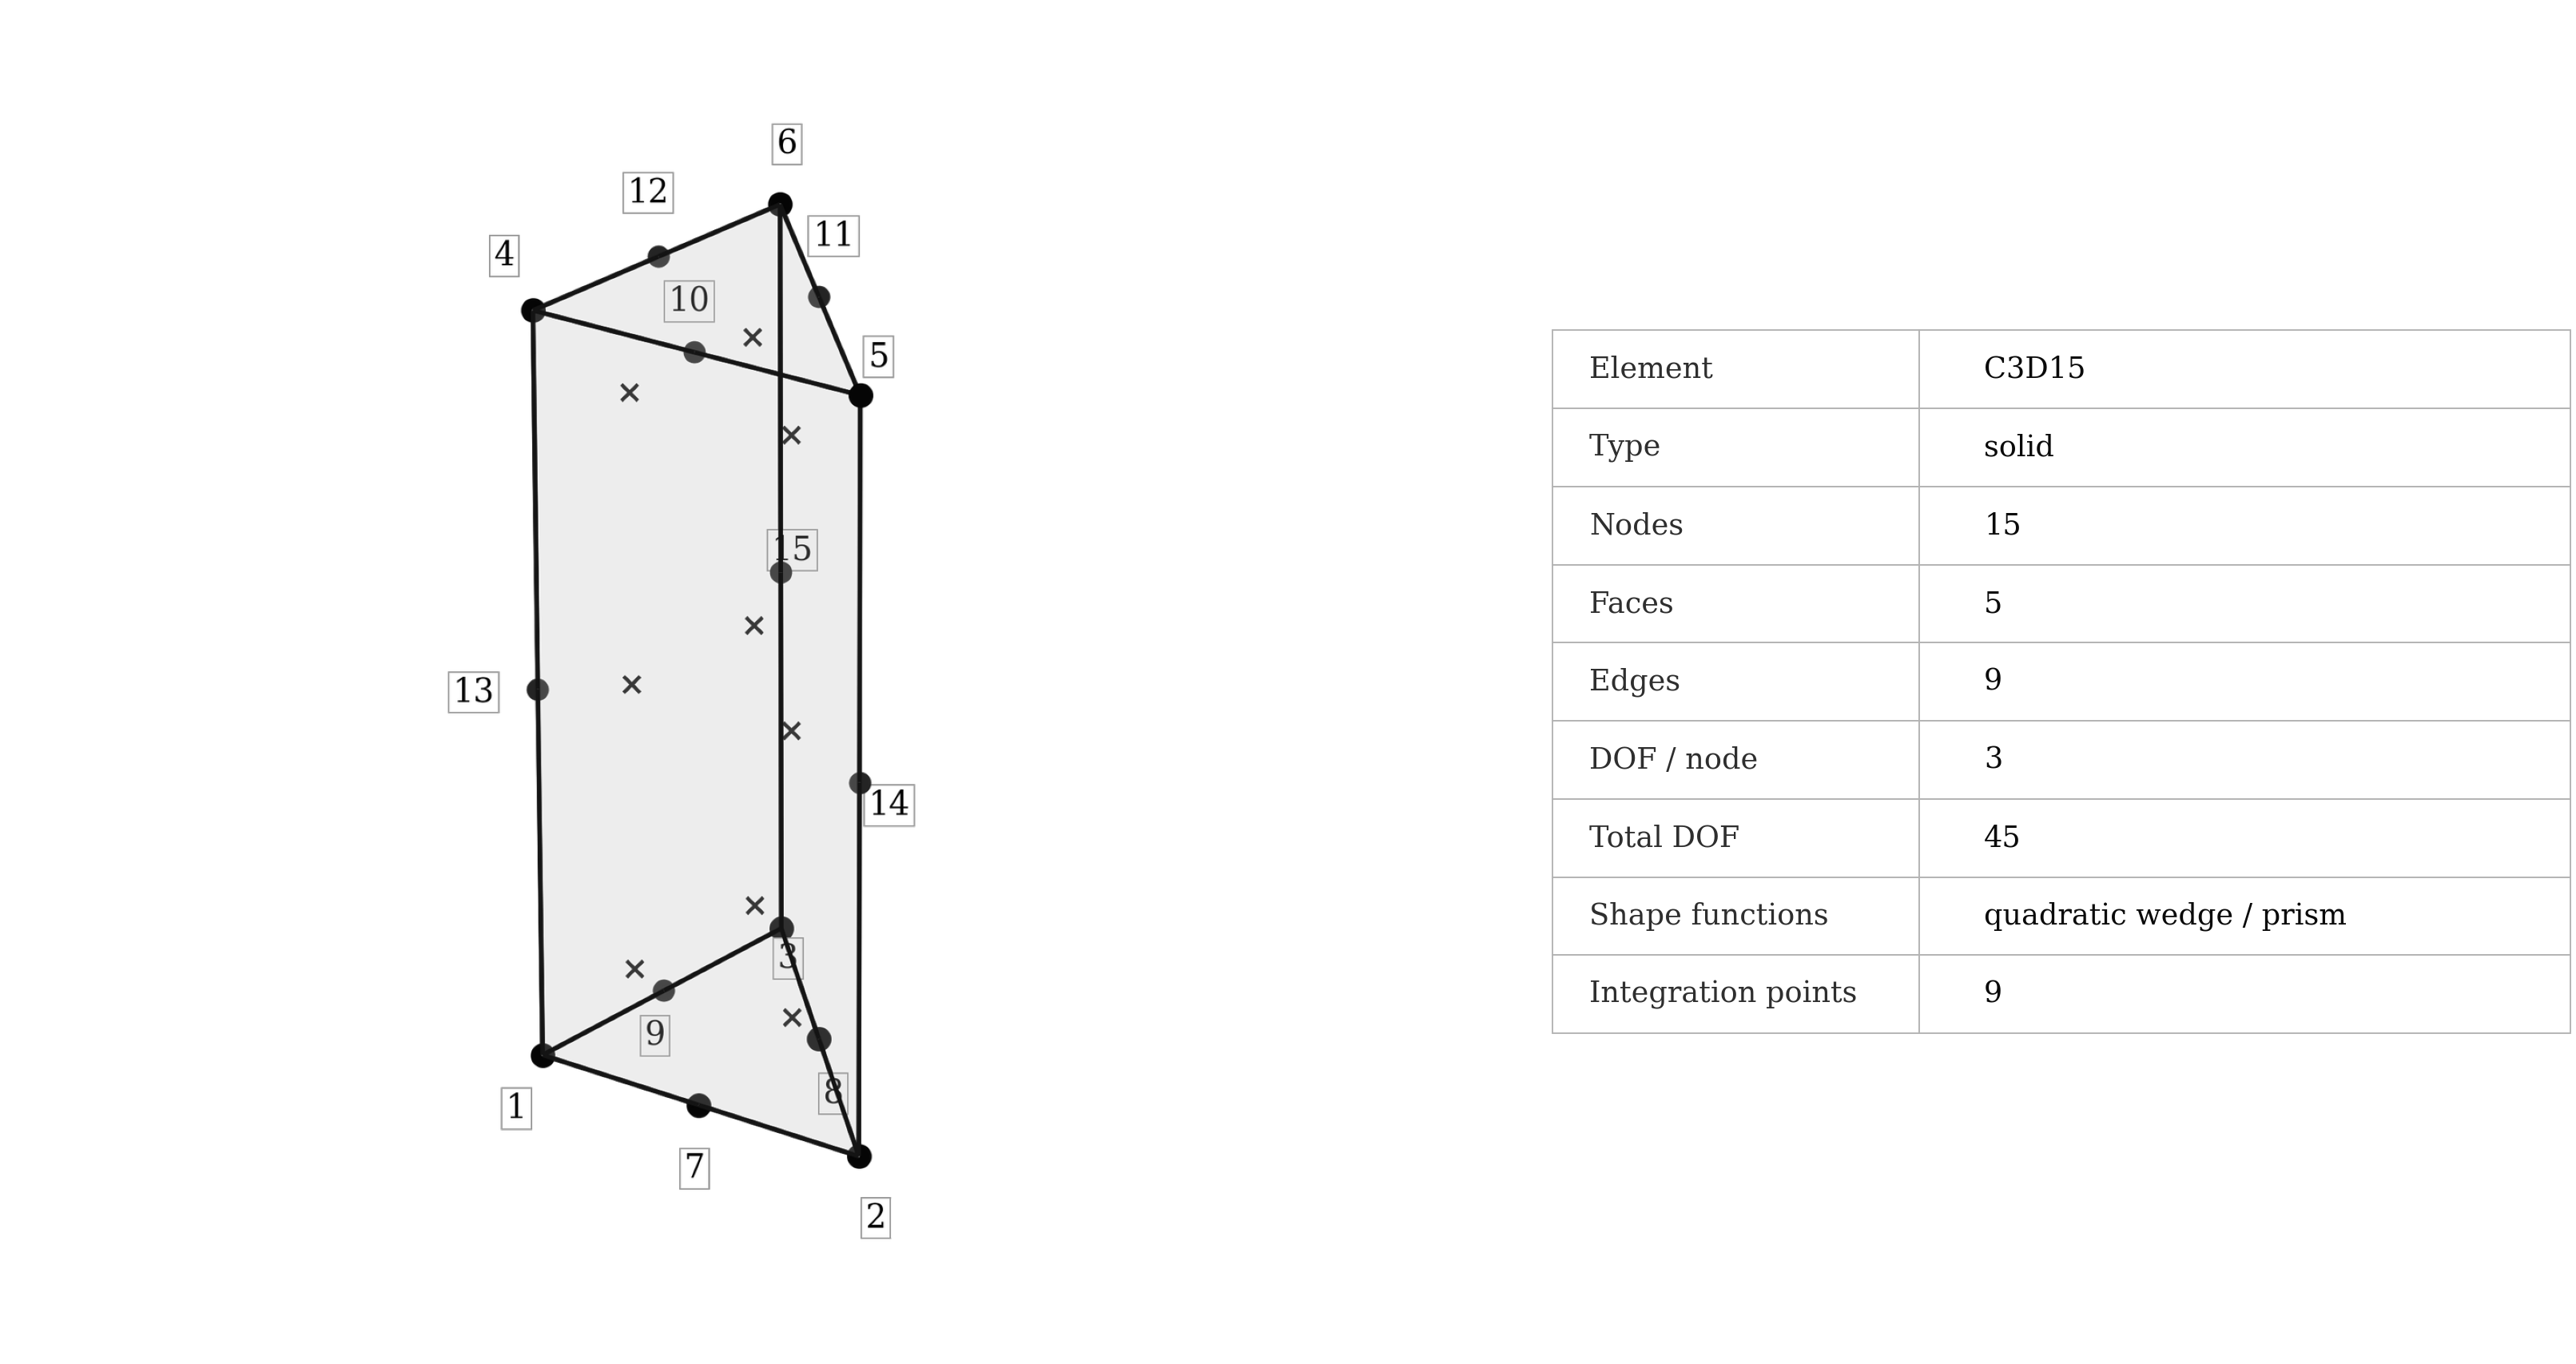
\includegraphics[width=0.80\linewidth]{pages/figures/element_schematics/c3d15_schematic.png}
    \caption{\val{C3D15} quadratic wedge element.}
\end{figure}

\begin{syntax}
*ELEMENT, TYPE=C3D15, ELSET=<set>
<id>, <n1>, ..., <n15>
\end{syntax}

\val{C3D15} is the quadratic counterpart of the six-node wedge. It adds midside nodes and represents curvature, bending, and through-thickness gradients at higher order than \val{C3D6}. Its topology matches higher-order swept meshes and prismatic regions created by extruding a quadratic triangular surface mesh.

The element combines wedge topology with higher-order through-thickness interpolation. Curved swept solids, local layered regions, and transition zones can therefore require fewer elements than with \val{C3D6}.

Higher-order mapping increases sensitivity to midside-node placement. Poorly shaped triangular end faces, excessive twisting of the side faces, and midside nodes that depart from the intended geometry degrade the mapping. A high-order wedge with a poor mapping is not automatically more accurate than a clean low-order mesh.

\val{C3D15} represents quadratic wedge meshes. A structured quadratic hexahedral mesh provides the more regular \val{C3D20} topology where geometry permits it, whereas \val{C3D10} supports fully unstructured complex geometry.

\clearpage
\paragraph{\val{C3D20}: 20-node quadratic hexahedral solid}

\begin{figure}[H]
    \centering
    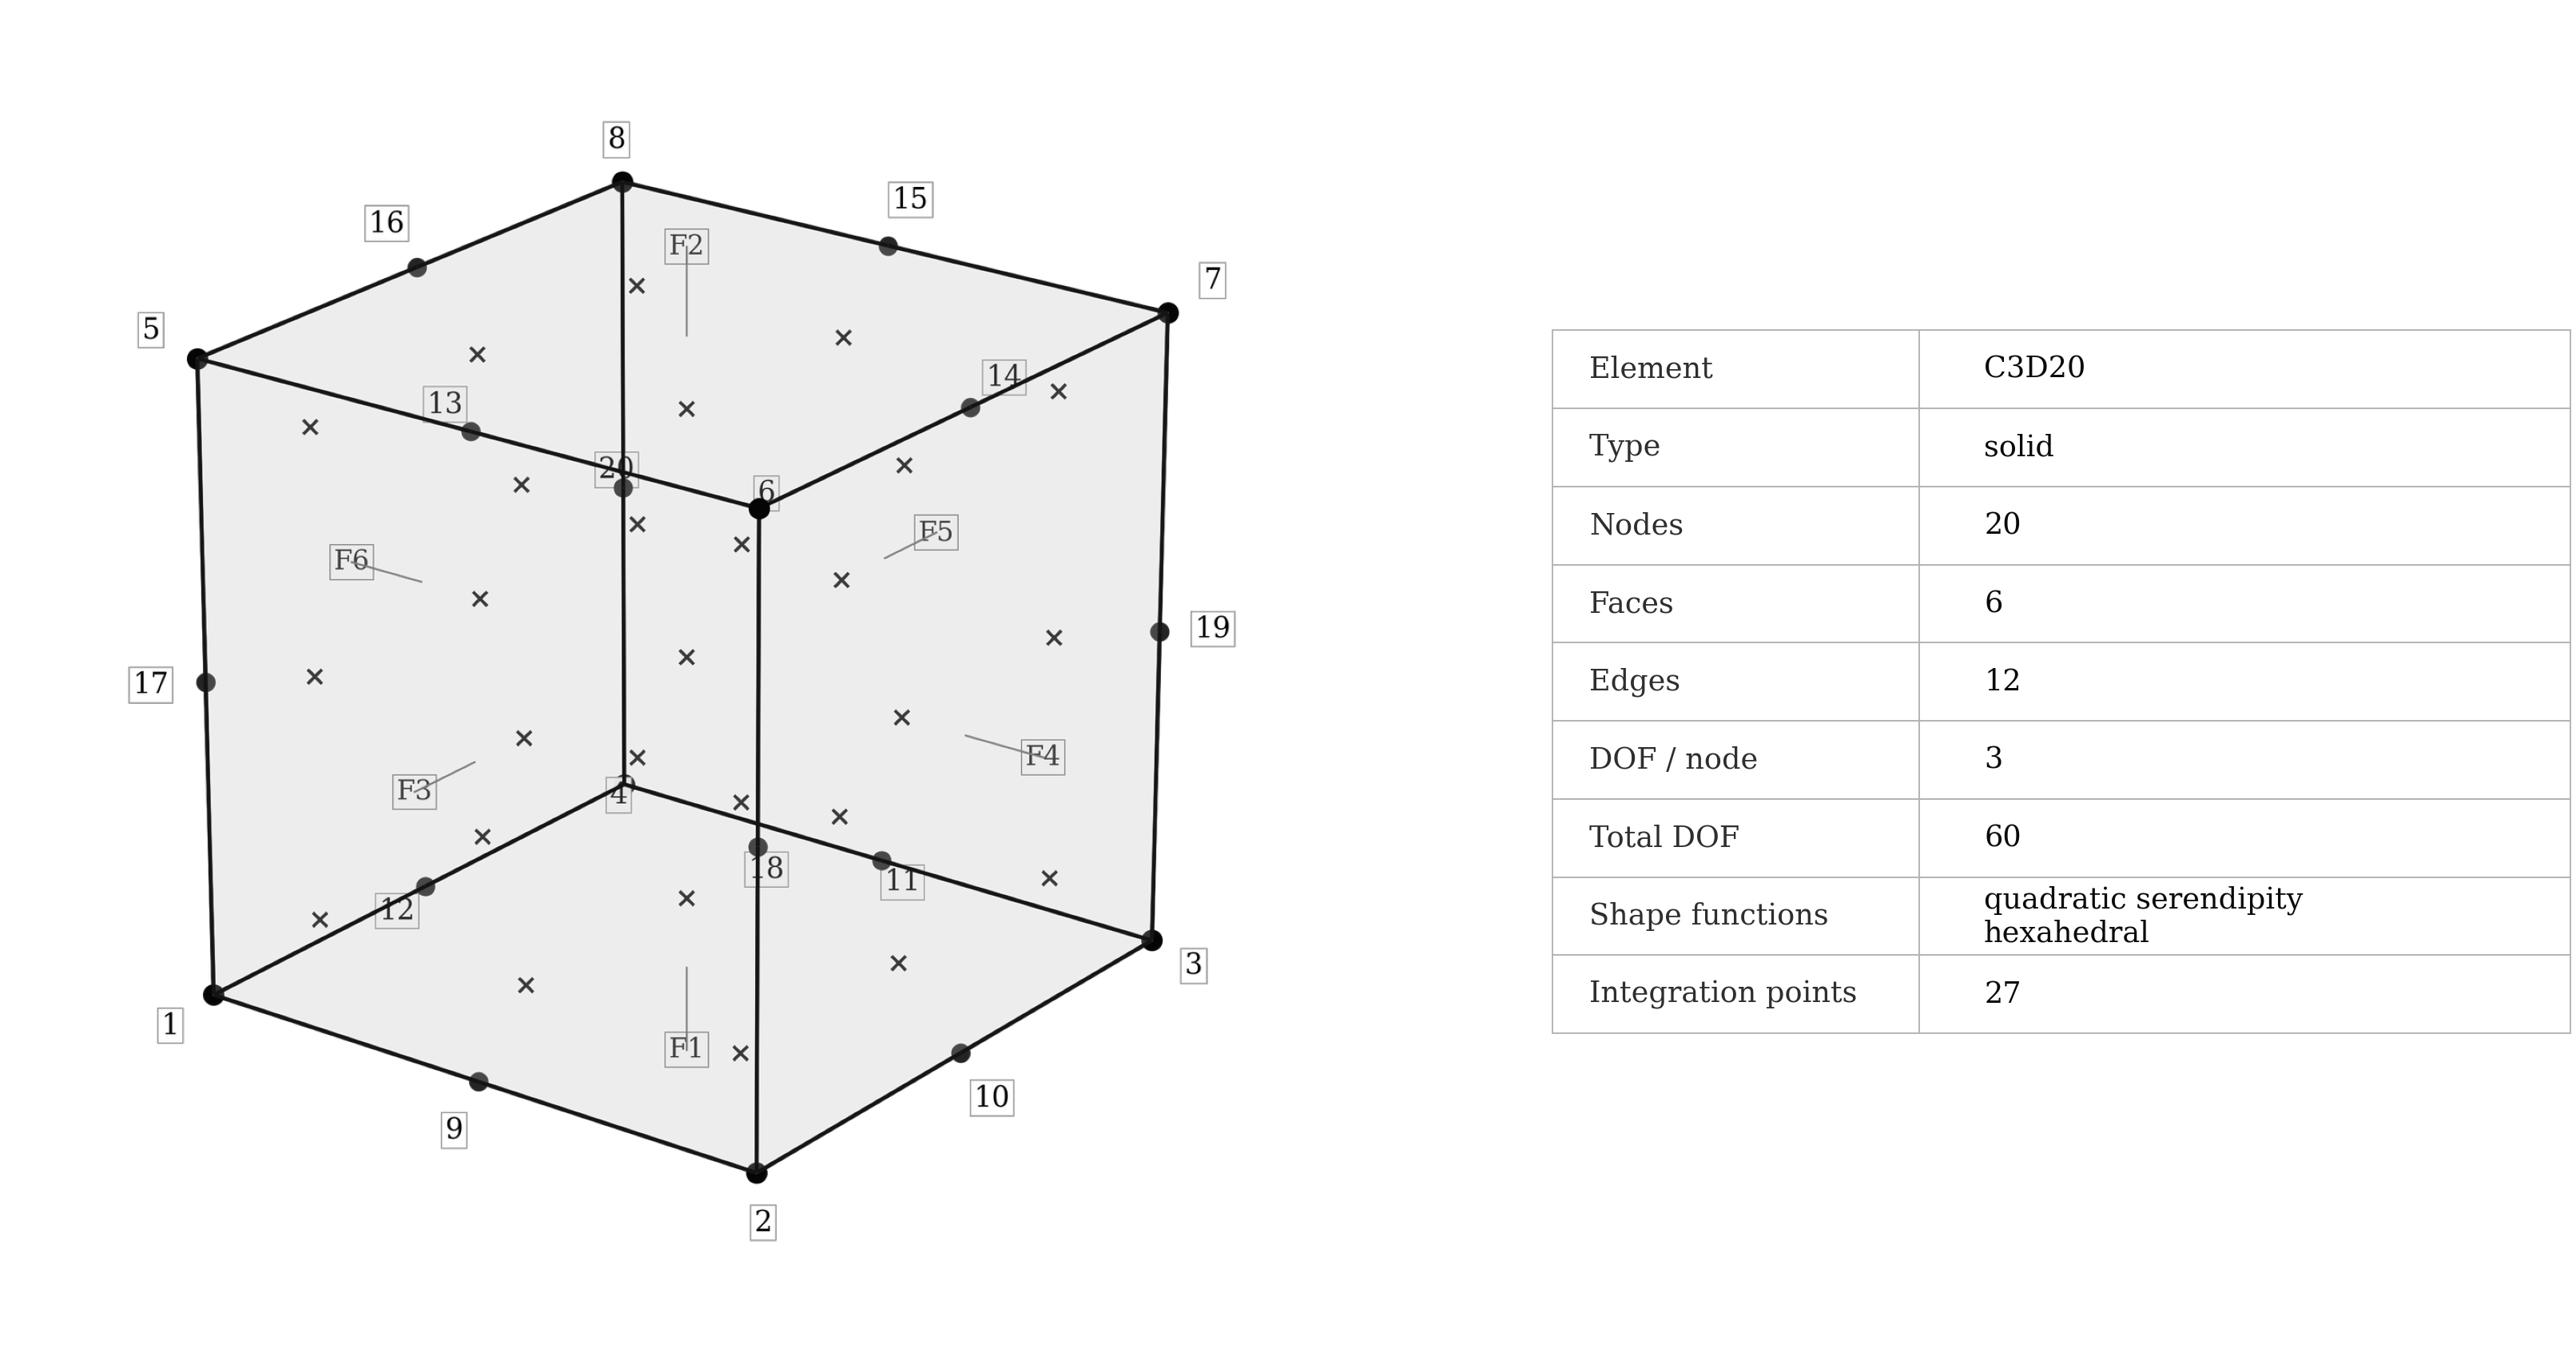
\includegraphics[width=0.82\linewidth]{pages/figures/element_schematics/c3d20_schematic.png}
    \caption{\val{C3D20} quadratic hexahedral element.}
\end{figure}

\begin{syntax}
*ELEMENT, TYPE=C3D20, ELSET=<set>
<id>, <n1>, ..., <n20>
\end{syntax}

\val{C3D20} is the full-integration quadratic hexahedral solid. The eight corner nodes are supplemented by twelve midside nodes, giving the element higher-order bending and stress-gradient representation than \val{C3D8}. Curved geometry is also represented at higher order when midside nodes follow the physical boundary.

For smooth structural fields and high-quality structured meshes, \val{C3D20} provides high-order solid accuracy. Its quadratic hexahedral interpolation represents curved blocks, swept volumes, thick structural regions, and smooth stress gradients.

The main costs are larger element matrices and stricter geometric quality requirements. Distortion of a quadratic mapping can be more harmful than distortion of a linear one because the midside nodes participate directly in the geometry interpolation. Jacobian quality therefore depends on both corner and midside-node positions.

Relative to \val{C3D8}, \val{C3D20} exchanges larger element matrices for higher-order accuracy. A fine regular \val{C3D8} mesh can remain less expensive for models dominated by linear global stiffness.

\clearpage
\paragraph{\val{C3D20R}: 20-node reduced-integration hexahedral solid}

\begin{figure}[H]
    \centering
    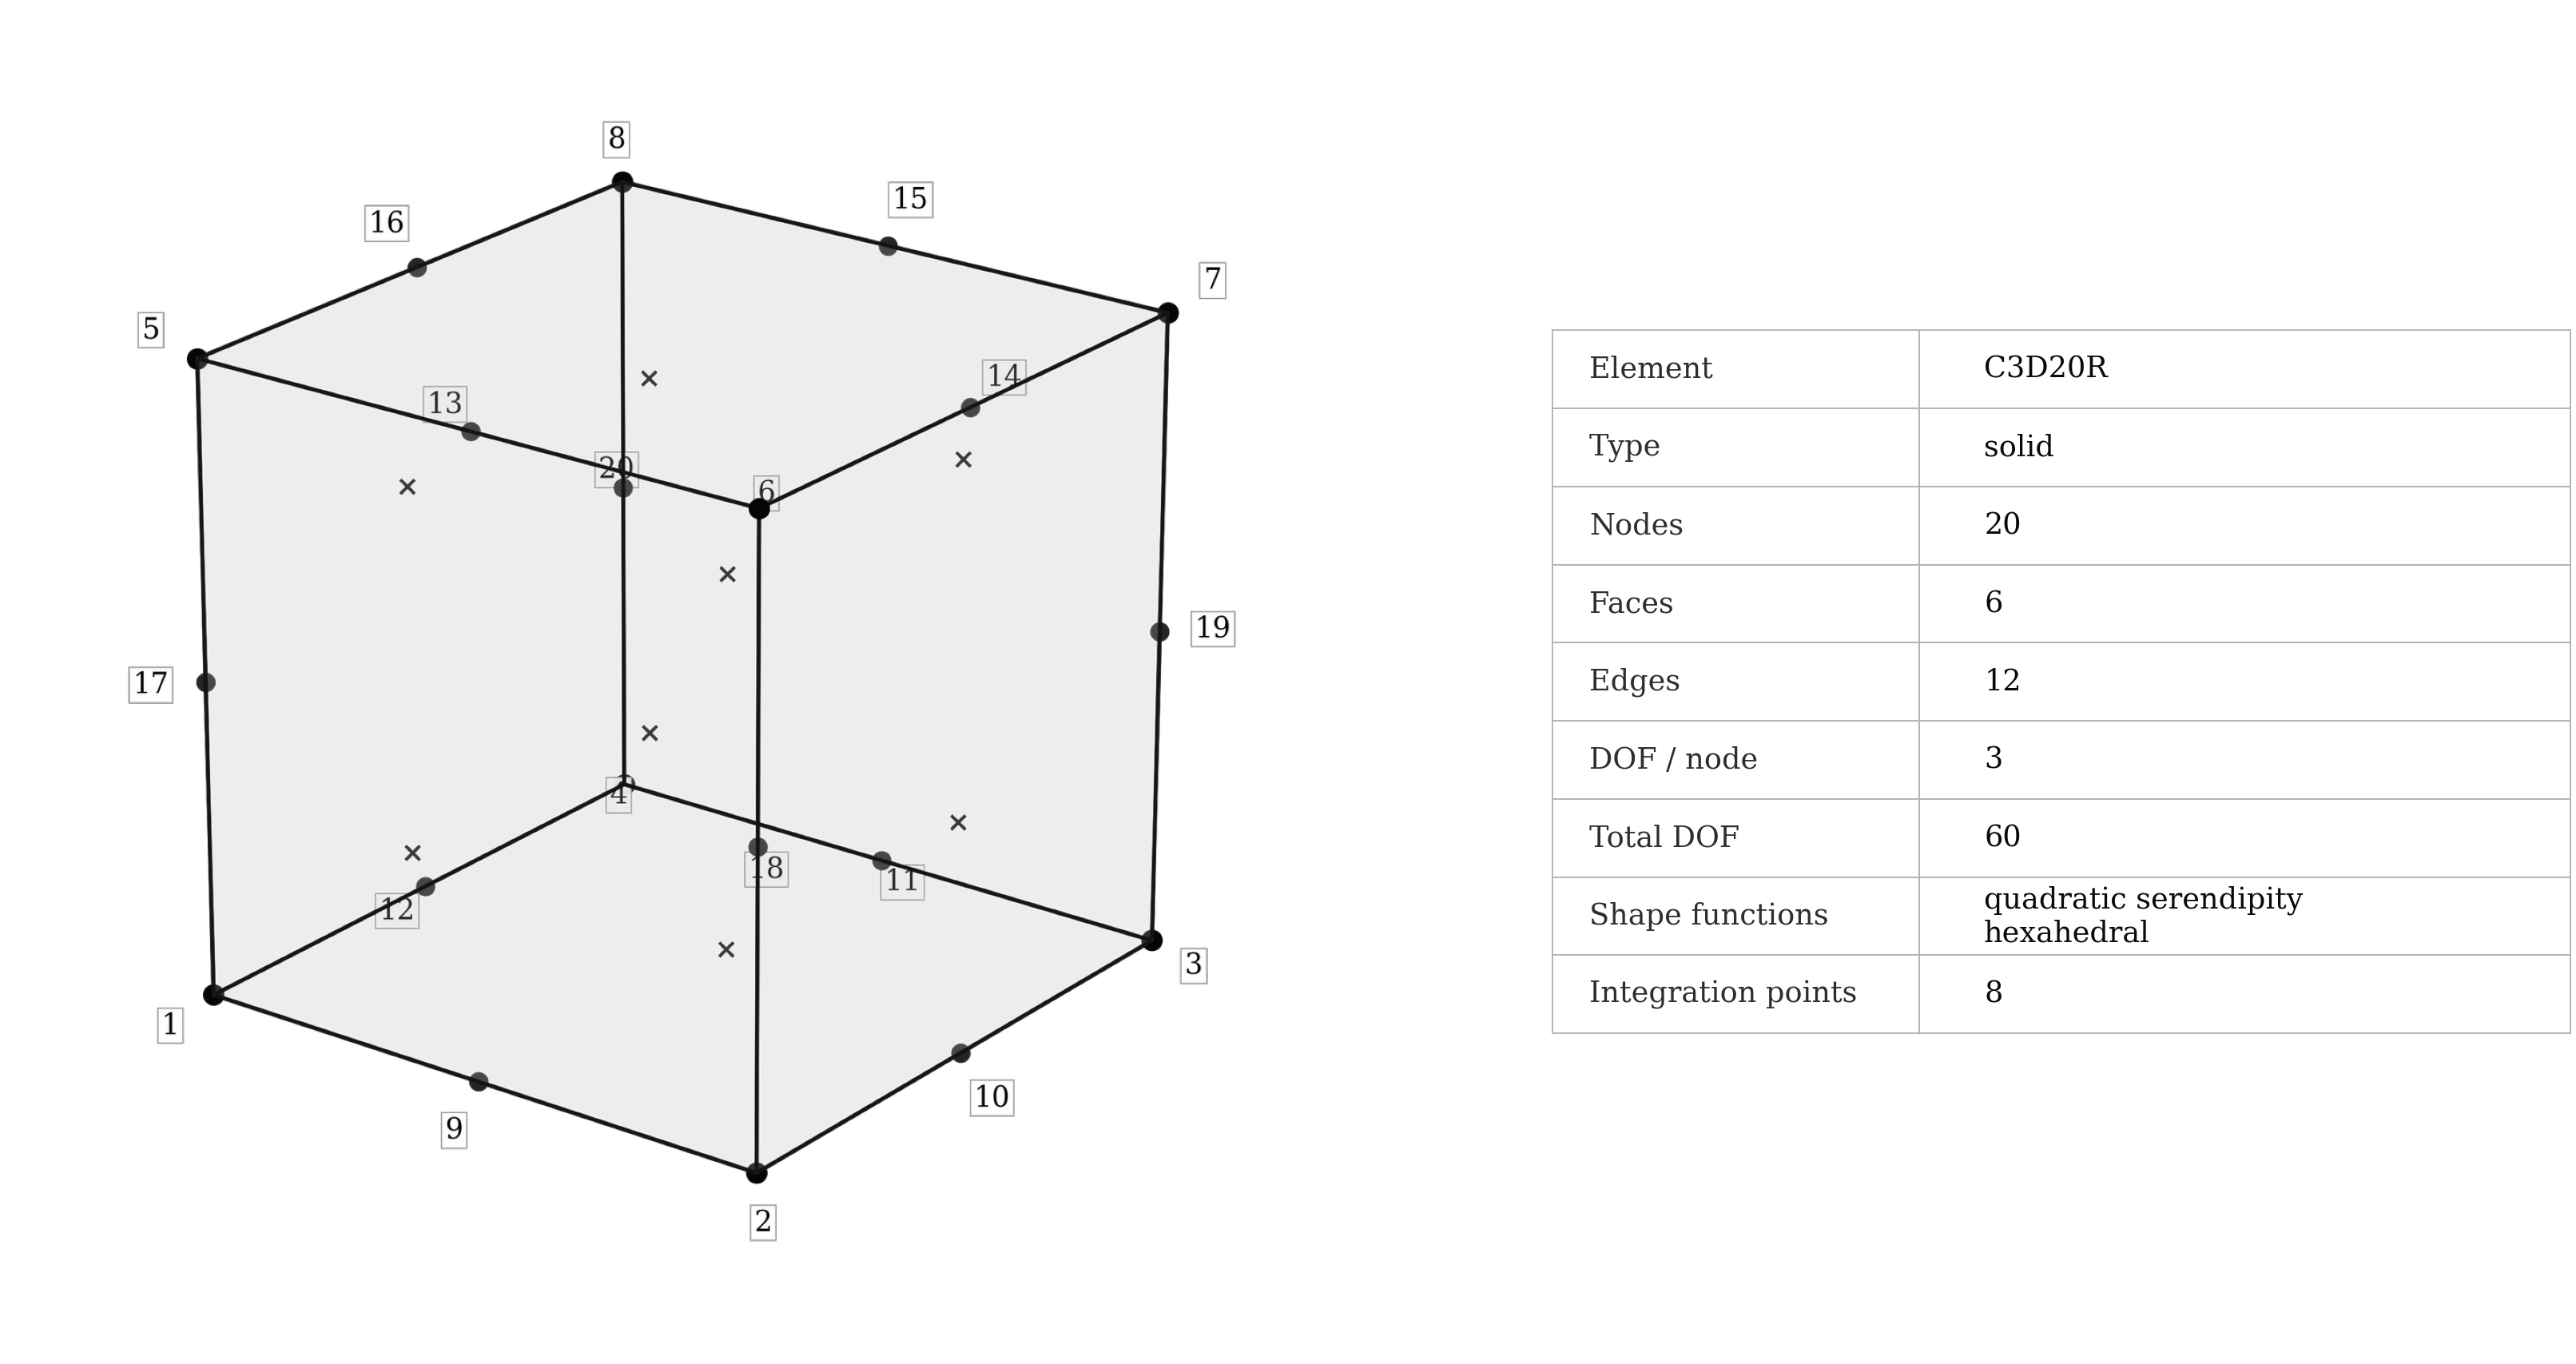
\includegraphics[width=0.82\linewidth]{pages/figures/element_schematics/c3d20r_schematic.png}
    \caption{\val{C3D20R} reduced-integration quadratic hexahedral solid element.}
\end{figure}

\begin{syntax}
*ELEMENT, TYPE=C3D20R, ELSET=<set>
<id>, <n1>, ..., <n20>
\end{syntax}

\val{C3D20R} uses the same twenty-node topology and quadratic interpolation as \val{C3D20}, but the stiffness contribution is evaluated with reduced integration. The reduced rule lowers cost and can improve behaviour in states where full integration introduces excessive constraint or stiffness.

Reduced integration changes the numerical character of the element; it is not merely a faster switch. Nonphysical low-energy deformation modes and sensitivity to mesh distortion can appear in deformed shapes, reaction balance, strain-energy distribution, and comparison with \val{C3D20}.

The formulation combines a quadratic hexahedral mesh with reduced integration. \val{C3D20} provides the corresponding fully integrated comparison formulation.

Solid stress and strain recovery is performed at the constitutive integration points and then extrapolated to element nodes; global nodal results are averaged over element contributions. An element with fewer integration points cannot provide the same recovered spatial variation as its full-integration counterpart. See Section~\ref{sec:output-results} for the distinction between integration-point, element-nodal, and averaged nodal fields.

\clearpage
\subsubsection{Shell elements}

Shell elements model thin-walled structures through a two-dimensional
reference surface with an assigned thickness or generalized sectional
stiffness. Their kinematics represent membrane stretching, bending,
and transverse shear without discretizing the thickness with
continuum elements. FEMaster's finite-rotation shells use independent
nodal translations and rotations, so the current orientation of
the shell can be represented directly. Typical applications include
plates, aircraft skins, curved panels, and other lightweight
structures dominated by midsurface deformation.

The recovered quantities include membrane forces, bending moments,
transverse-shear resultants, and supported top/bottom stresses, but
not an arbitrary three-dimensional through-thickness stress field.
A solid model may be more suitable near concentrated load
introductions, connections, or locations with significant thickness
effects. The shell normal determines the top/bottom convention,
affects pressure direction, and enters the interpretation of bending
results. Mesh quality, surface orientation, thickness, and material
directions must therefore be defined consistently.

Four finite-rotation formulations are available, covering triangular
and quadrilateral topologies with linear and quadratic geometric
interpolation. Triangular meshes accommodate irregular boundaries,
while quadrilateral meshes are particularly effective on structured
surfaces. Higher-order elements resolve smooth curvature more
efficiently but increase element cost and require well-positioned
midside nodes. Each heading lists all accepted aliases of the same
FEMaster implementation.

\clearpage
\paragraph{\val{MITC3FRT} / \val{S3} / \val{S3R}: 3-node finite-rotation triangular shell}

\begin{figure}[H]
    \centering
    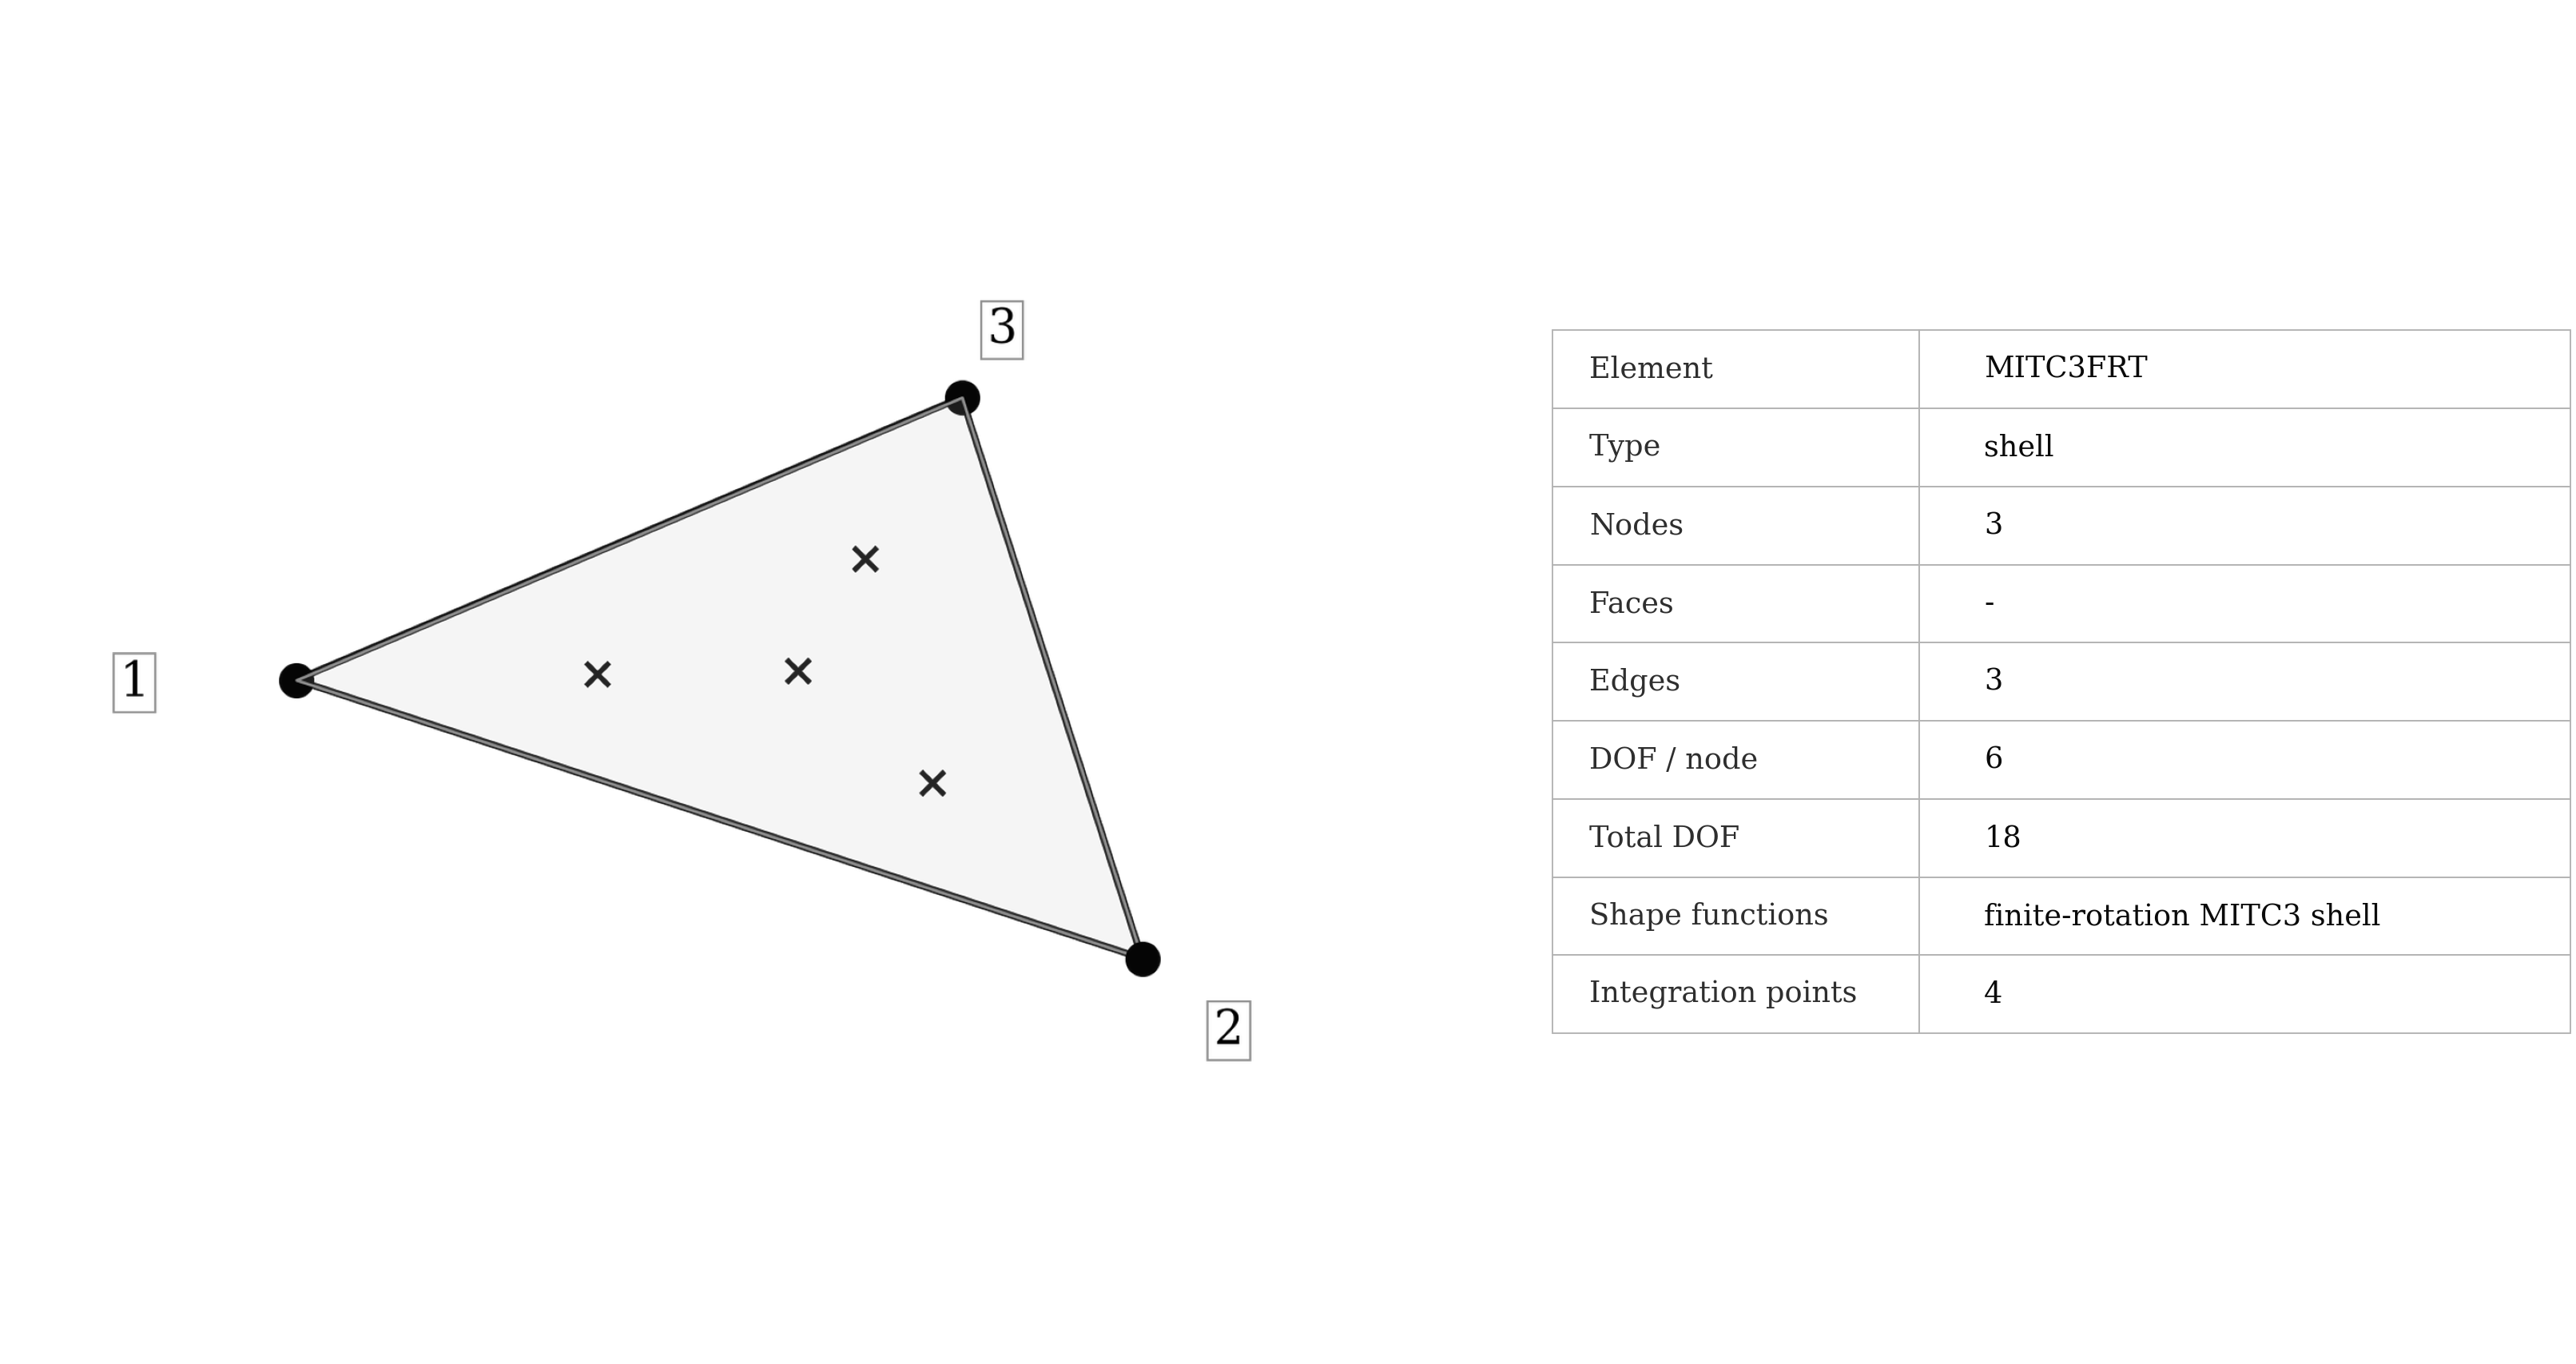
\includegraphics[width=0.76\linewidth]{pages/figures/element_schematics/mitc3frt_schematic.png}
    \caption{Three-node finite-rotation triangular shell geometry and node ordering.}
\end{figure}

\begin{syntax}
*ELEMENT, TYPE=MITC3FRT, ELSET=<set>
<id>, <n1>, <n2>, <n3>
\end{syntax}

The three-node triangular shell combines a linear geometric
interpolation with finite-rotation kinematics and independent nodal
translations and rotations. It represents membrane deformation,
bending, and transverse shear within the common shell framework.
This compact topology is useful for unstructured surface meshes,
irregular boundaries, openings, and transitions where a regular
quadrilateral mesh would be difficult to construct.

A single linear triangle has limited resolution of curved geometry
and spatially varying bending fields. Bending-dominated or strongly
curved models therefore require refinement, with convergence checked
using displacements, stresses or shell resultants, and strain energy.
The aliases \val{S3} and \val{S3R} select the same implementation as
\val{MITC3FRT}; the \val{R} suffix does not select a separate
reduced-integration formulation in FEMaster.

\clearpage
\paragraph{\val{MITC4FRT} / \val{S4} / \val{S4R} / \val{MITC4}: 4-node finite-rotation quadrilateral shell}

\begin{figure}[H]
    \centering
    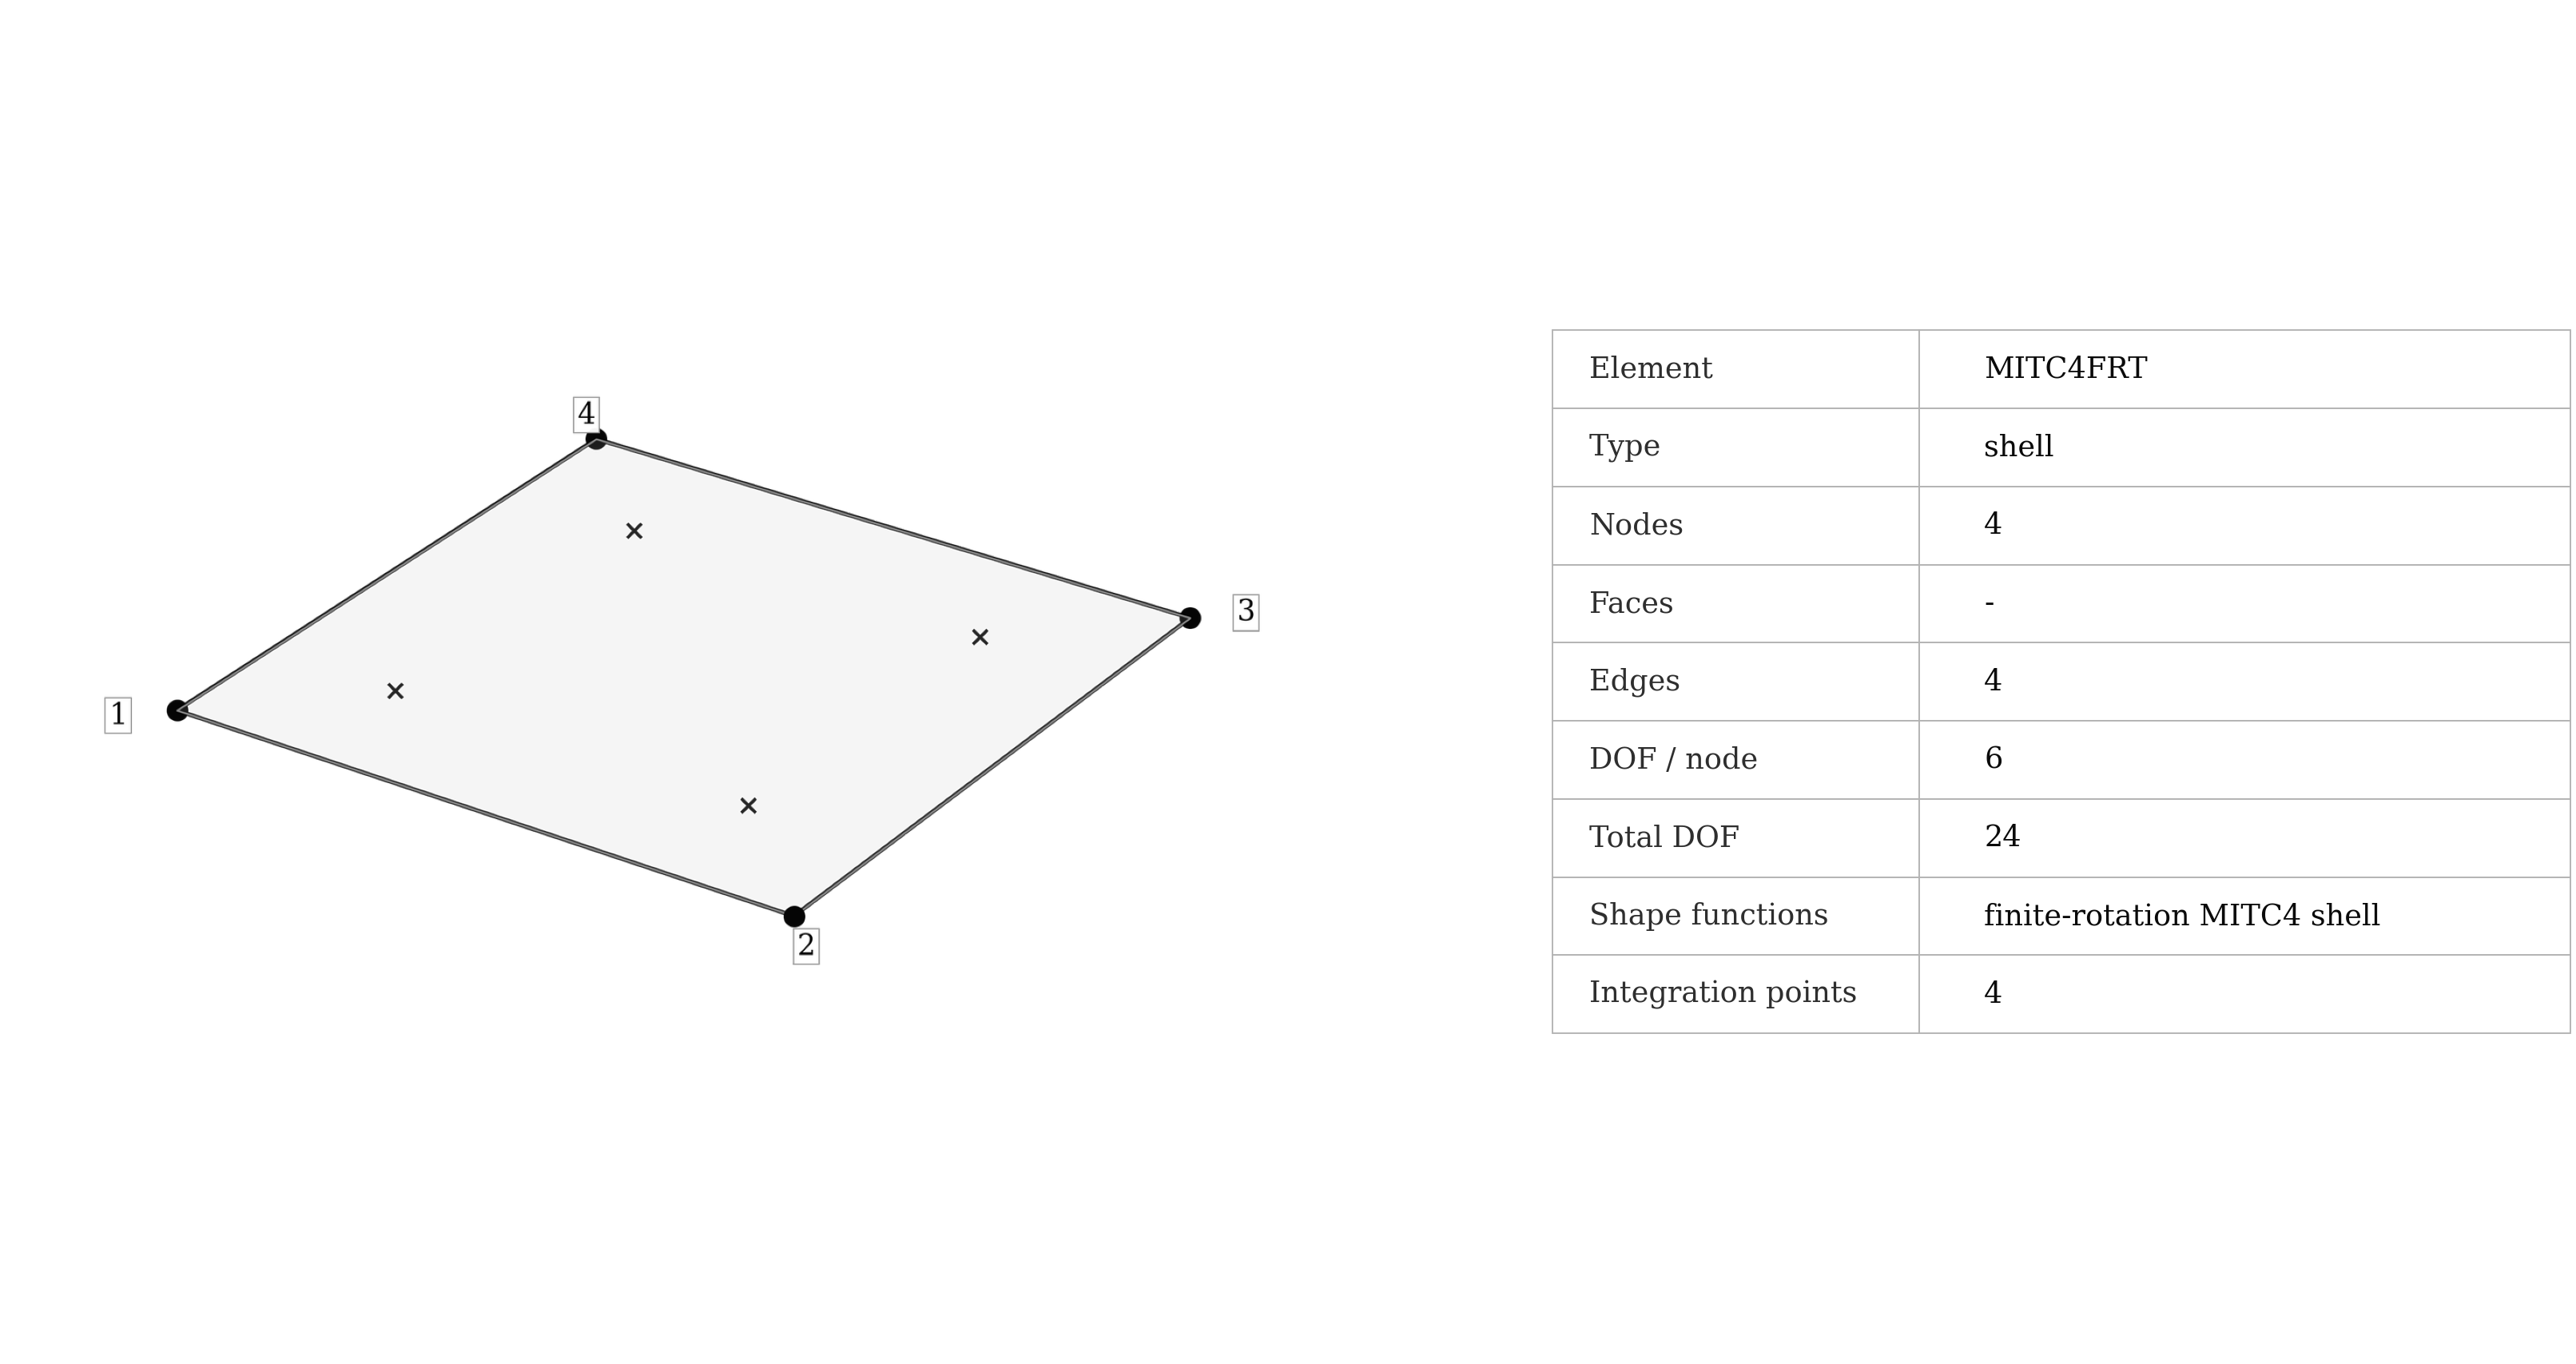
\includegraphics[width=0.78\linewidth]{pages/figures/element_schematics/mitc4frt_schematic.png}
    \caption{Four-node finite-rotation MITC shell geometry and node ordering.}
\end{figure}

\begin{syntax}
*ELEMENT, TYPE=MITC4FRT, ELSET=<set>
<id>, <n1>, <n2>, <n3>, <n4>
\end{syntax}

The four-node quadrilateral shell combines finite-rotation kinematics
with a Mixed Interpolation of Tensorial Components (MITC) treatment
of transverse shear. In thin-shell bending, an ordinary low-order
displacement interpolation can become artificially stiff because
the shear strains cannot approach their limiting values correctly.
This numerical effect, known as shear locking, is mitigated by the
MITC interpolation while transverse-shear deformation remains part
of the underlying shell model.

The formulation is well suited to plates, skins, stiffened panels,
and shell assemblies discretized with regular quadrilaterals. It
represents bending and twisting through independent nodal rotations
rather than an internally expanded solid mesh. Nevertheless, strong
warping, severe element skewness, and insufficient surface resolution
can reduce accuracy, especially for curved geometry and nonlinear
deformation paths. The names \val{S4}, \val{S4R}, and \val{MITC4}
are aliases for \val{MITC4FRT}; they do not select different
integration schemes.

\clearpage
\paragraph{\val{MITC6FRT} / \val{S6} / \val{S6R}: 6-node finite-rotation triangular shell}

\begin{figure}[H]
    \centering
    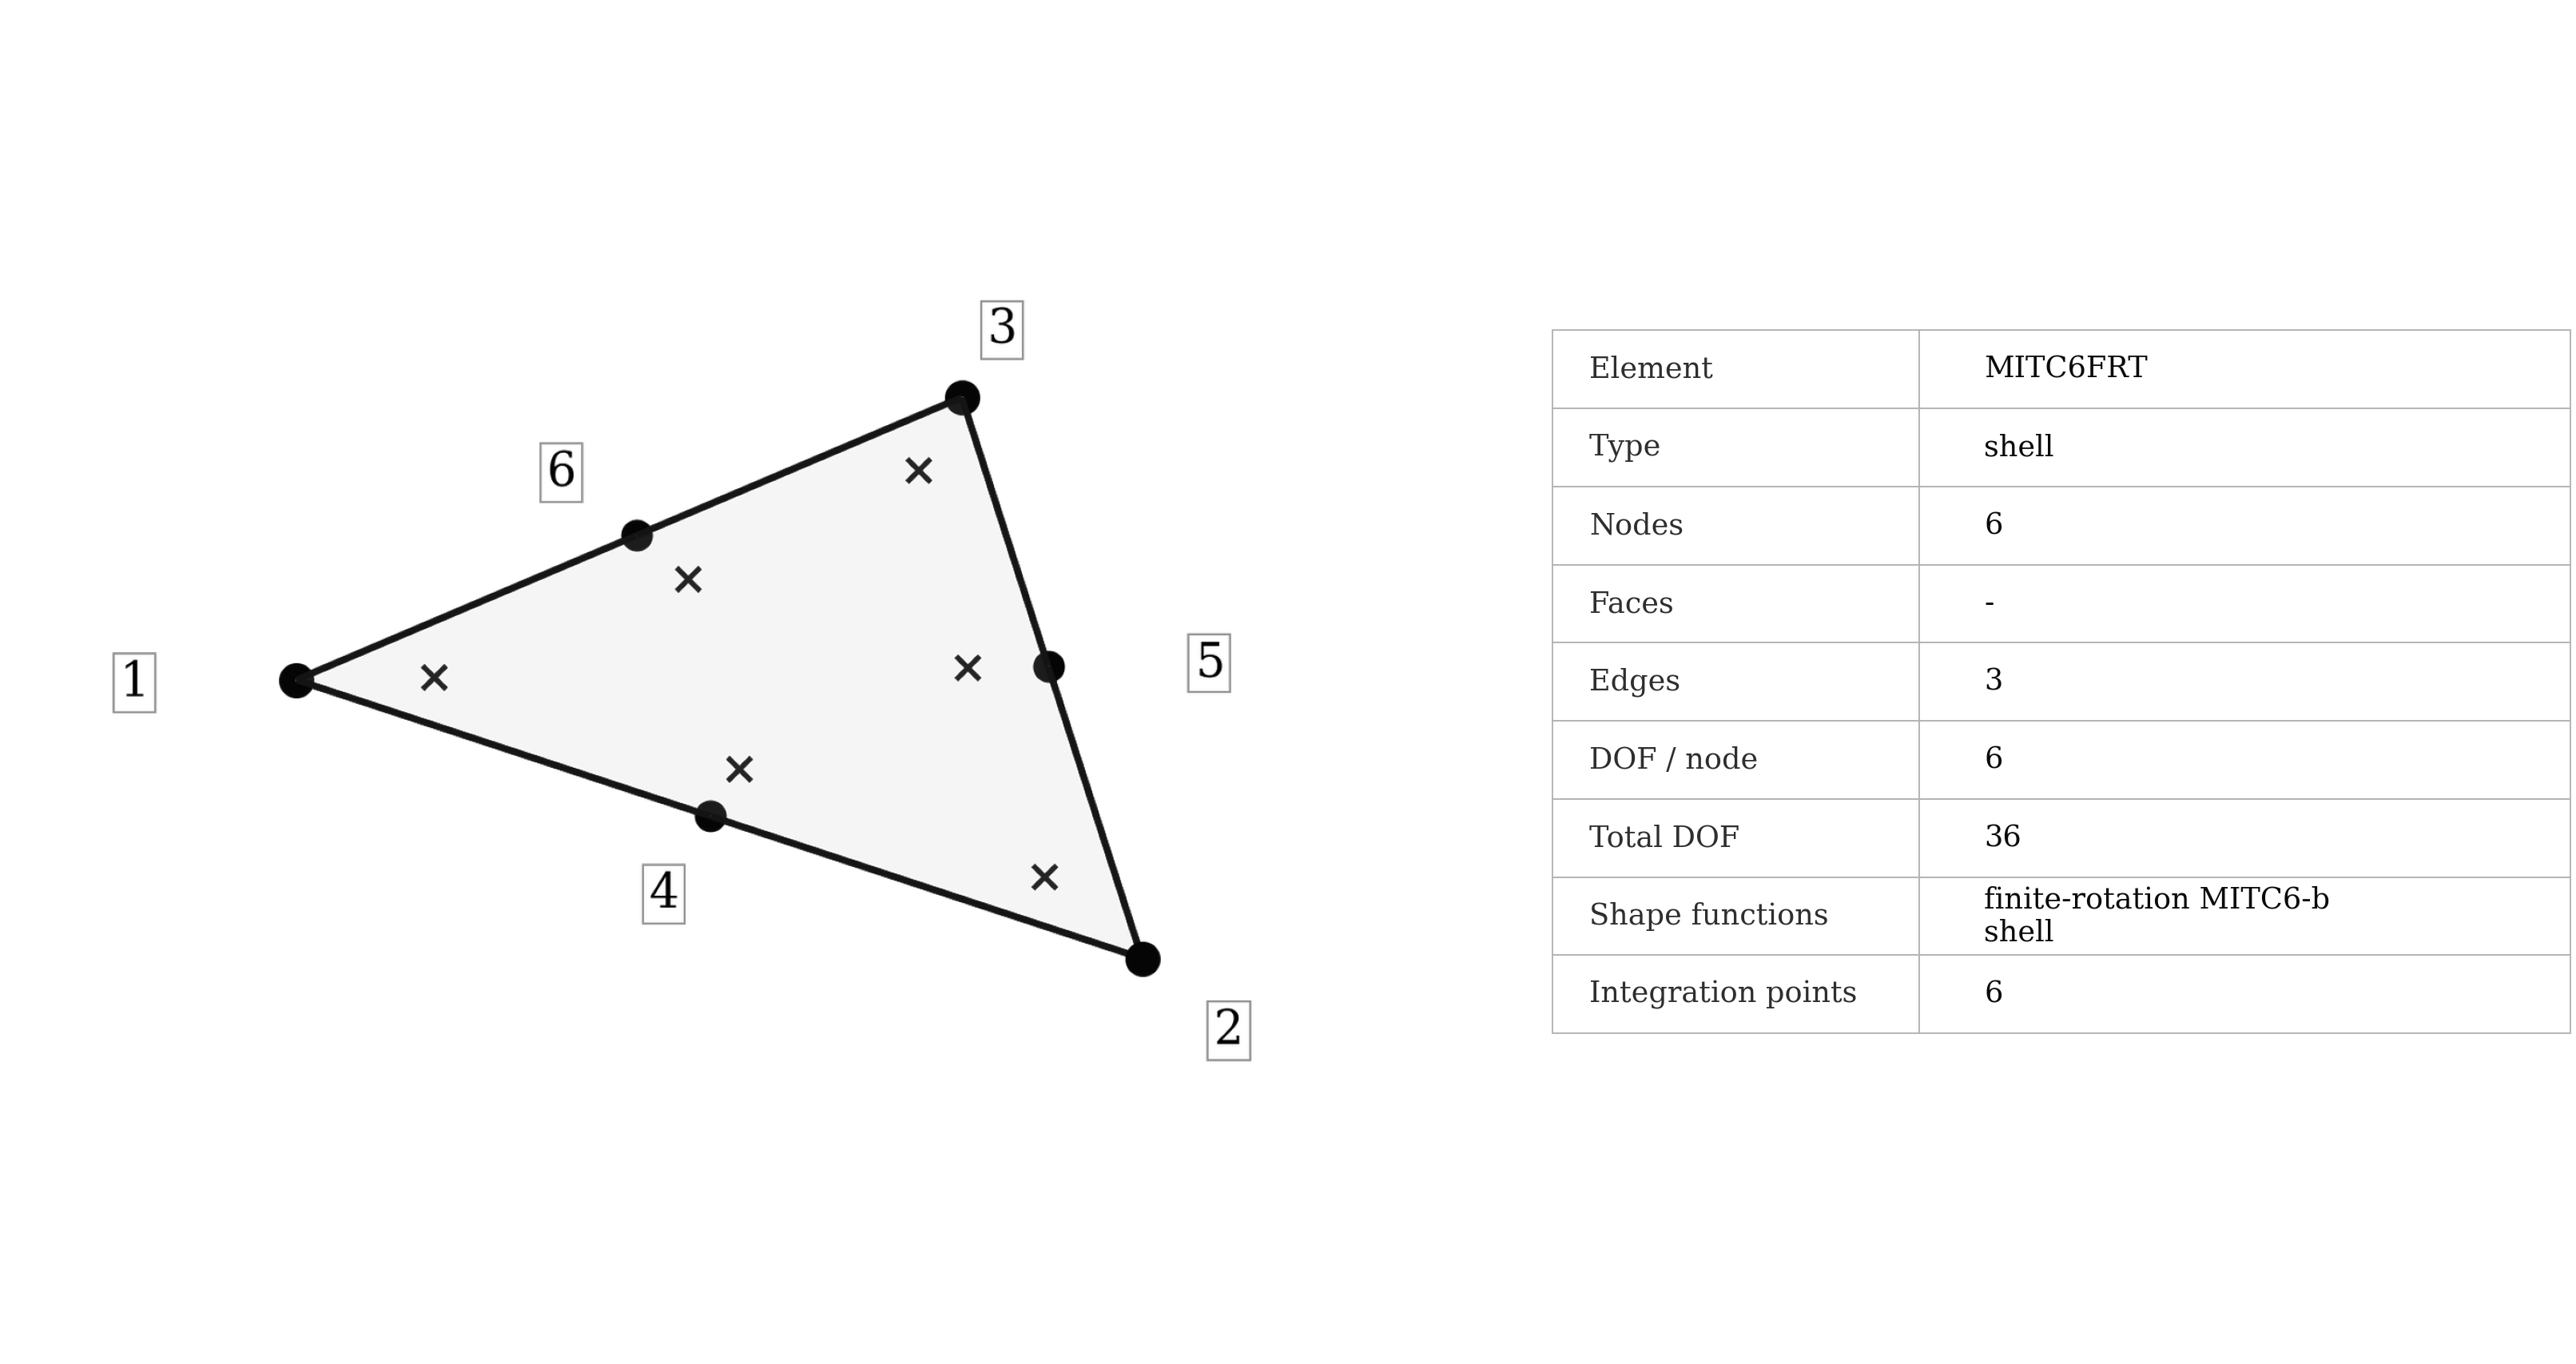
\includegraphics[width=0.78\linewidth]{pages/figures/element_schematics/mitc6frt_schematic.png}
    \caption{Six-node finite-rotation triangular shell geometry and node ordering.}
\end{figure}

\begin{syntax}
*ELEMENT, TYPE=MITC6FRT, ELSET=<set>
<id>, <n1>, <n2>, <n3>, <n4>, <n5>, <n6>
\end{syntax}

The six-node triangular shell extends the finite-rotation midsurface
description to quadratic geometric interpolation. Its midside nodes
allow curved edges and a more detailed representation of smoothly
varying displacement and bending fields than the three-node
triangle. It is useful for curved shell regions, cutouts, and
unstructured higher-order surface meshes where triangular topology
is preferred.

The higher interpolation order improves geometric flexibility but
does not eliminate sensitivity to mesh quality. Midside nodes must
follow the intended surface and highly distorted triangles can
produce inaccurate stiffness and recovered results. Thin-shell
bending calculations should therefore be checked by mesh
refinement. The \val{S6} and \val{S6R} aliases select exactly the
same FEMaster implementation as \val{MITC6FRT}.

\clearpage
\paragraph{\val{MITC8FRT} / \val{S8} / \val{S8R} / \val{MITC8}: 8-node finite-rotation quadrilateral shell}

\begin{figure}[H]
    \centering
    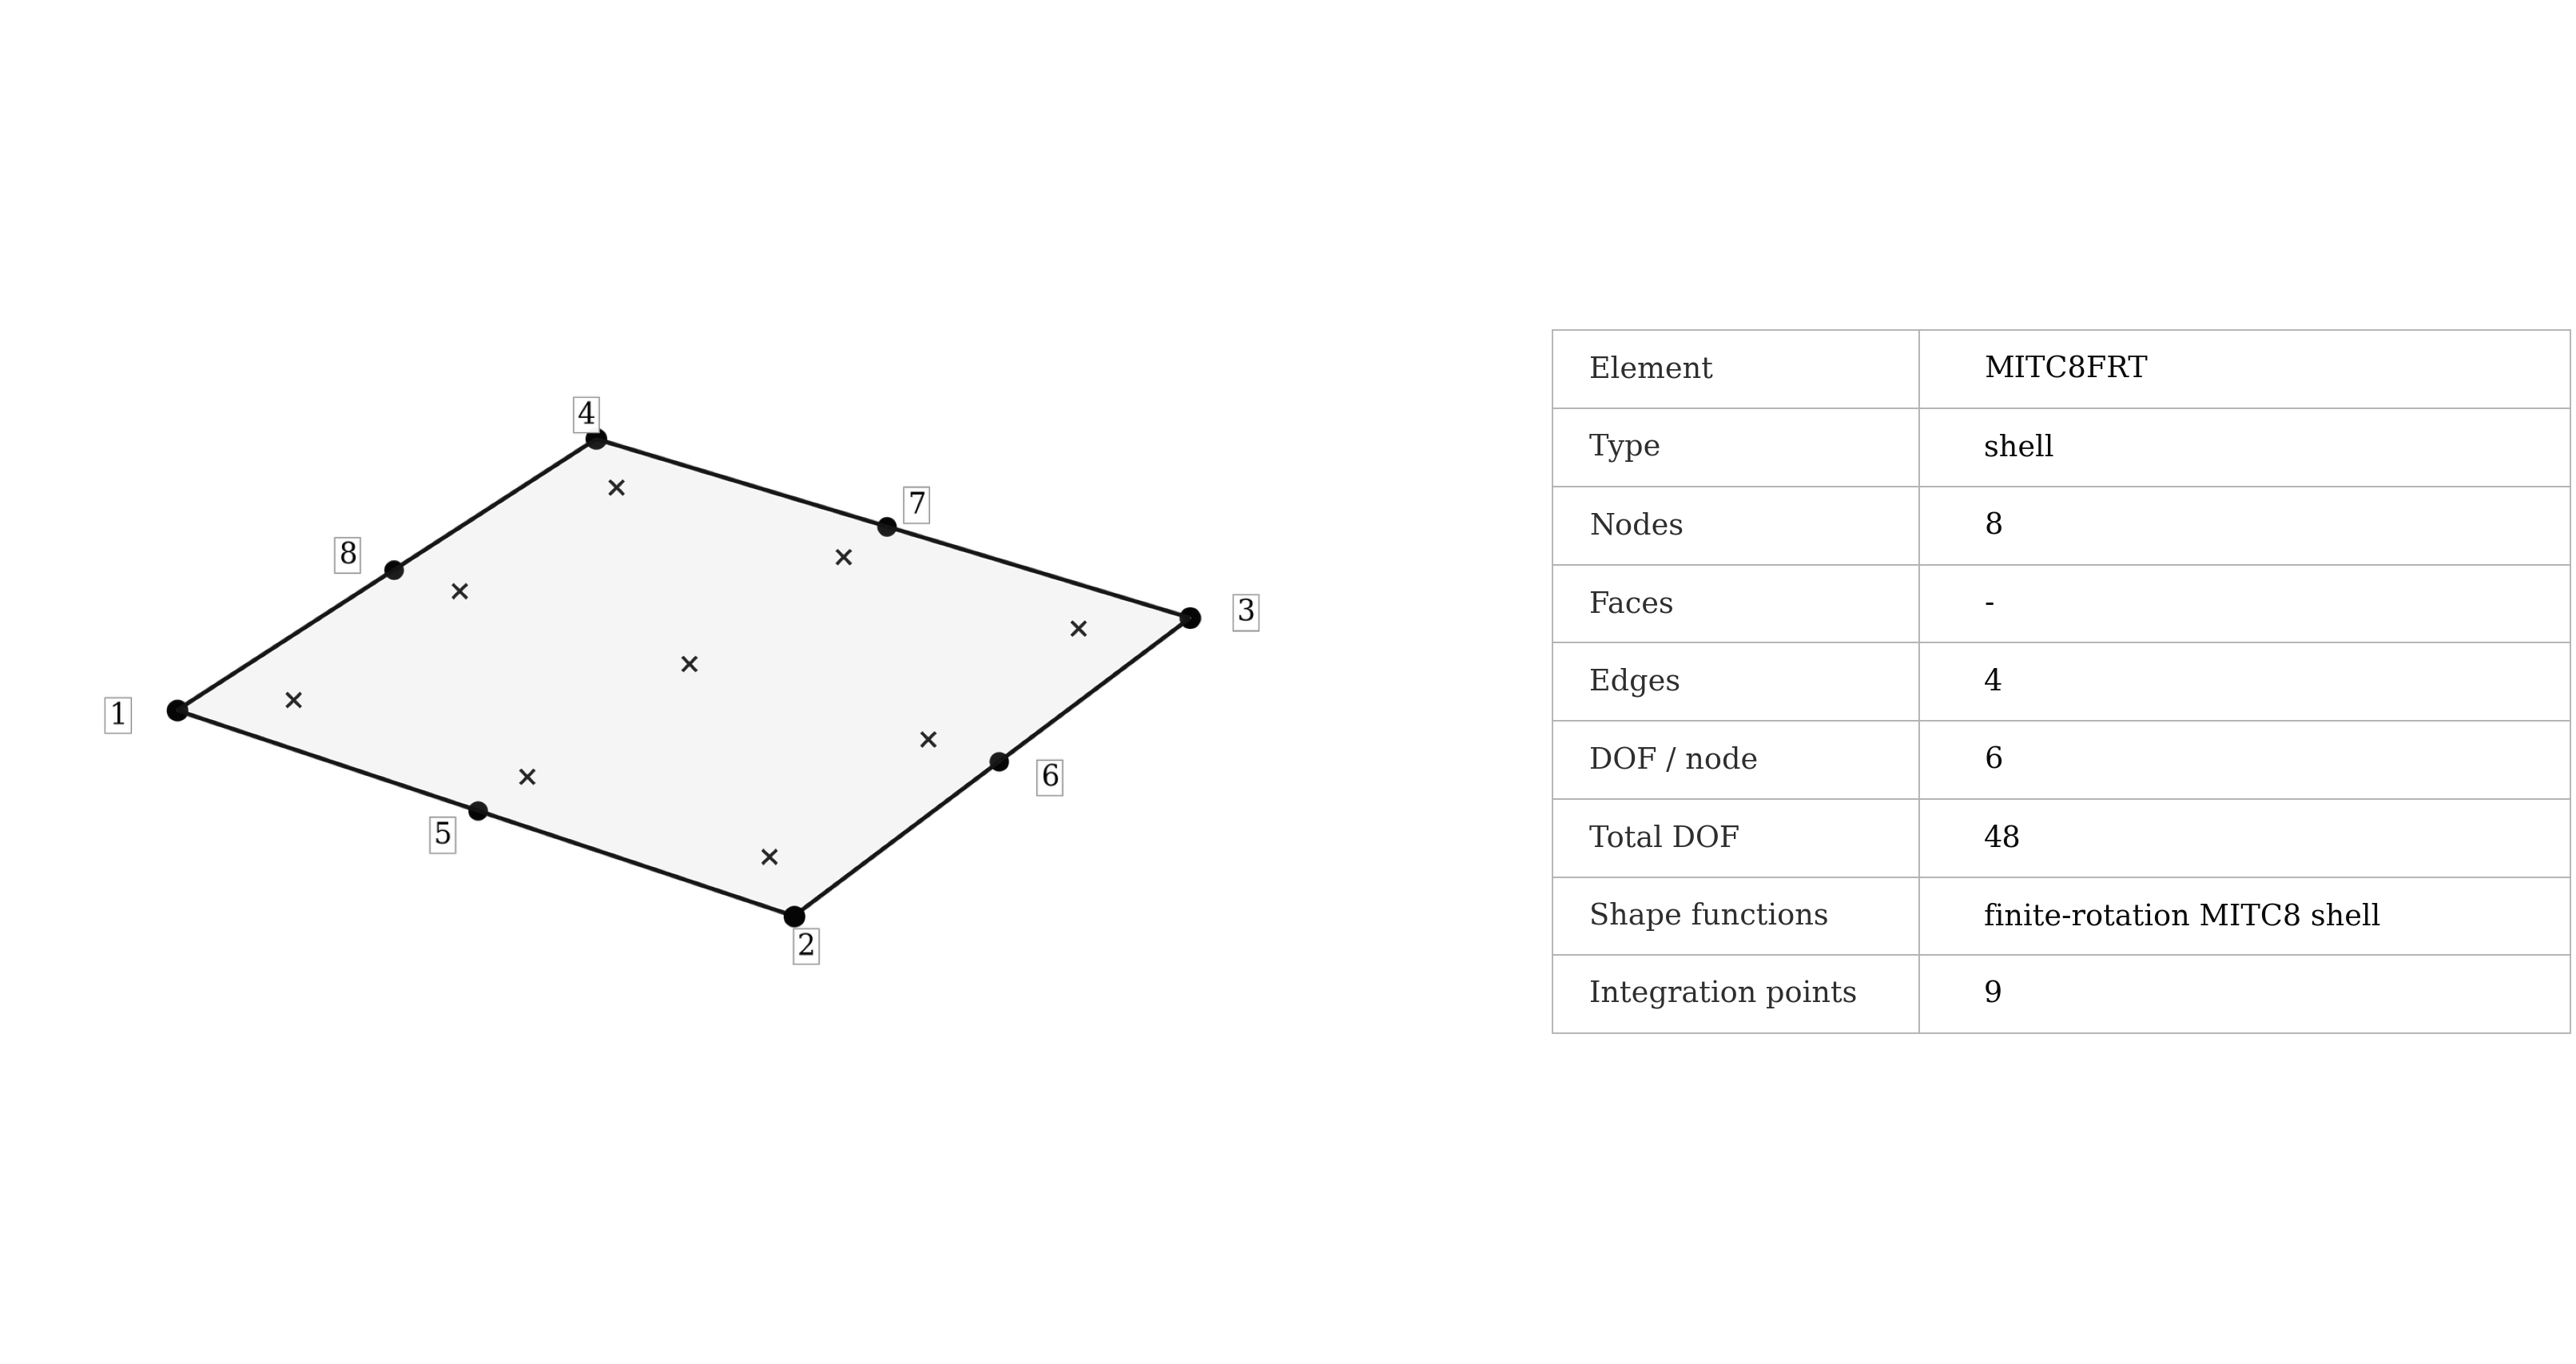
\includegraphics[width=0.80\linewidth]{pages/figures/element_schematics/mitc8frt_schematic.png}
    \caption{Eight-node finite-rotation MITC shell geometry and node ordering.}
\end{figure}

\begin{syntax}
*ELEMENT, TYPE=MITC8FRT, ELSET=<set>
<id>, <n1>, <n2>, <n3>, <n4>, <n5>, <n6>, <n7>, <n8>
\end{syntax}

The eight-node quadrilateral shell combines higher-order midsurface
interpolation, finite-rotation kinematics, and an MITC
transverse-shear treatment. The midside nodes provide a richer
description of smooth curvature, displacement, and bending fields
than the four-node element. This makes the formulation suitable
for curved panels and shell regions where accurate geometry and
smooth stress-resultant gradients are important.

Compared with \val{MITC4FRT}, the additional nodes increase
element cost but may reduce the number of elements needed for
smooth curved geometry. Accuracy still depends on the placement
of midside nodes, consistent shell normals, and acceptable element
warping. The shell idealization does not resolve detailed
through-thickness continuum stresses. The aliases \val{S8},
\val{S8R}, and \val{MITC8} select this same
\val{MITC8FRT} implementation.

Although grouped with the shell and panel formulations, \val{QSPT}
is a specialized shear-panel element rather than a general-purpose
shell. Its kinematics and recoverable quantities differ from those
of the finite-rotation MITC shells described above.

\clearpage
\paragraph{\val{QSPT}: quadrilateral shear-panel element}

\begin{figure}[H]
    \centering
    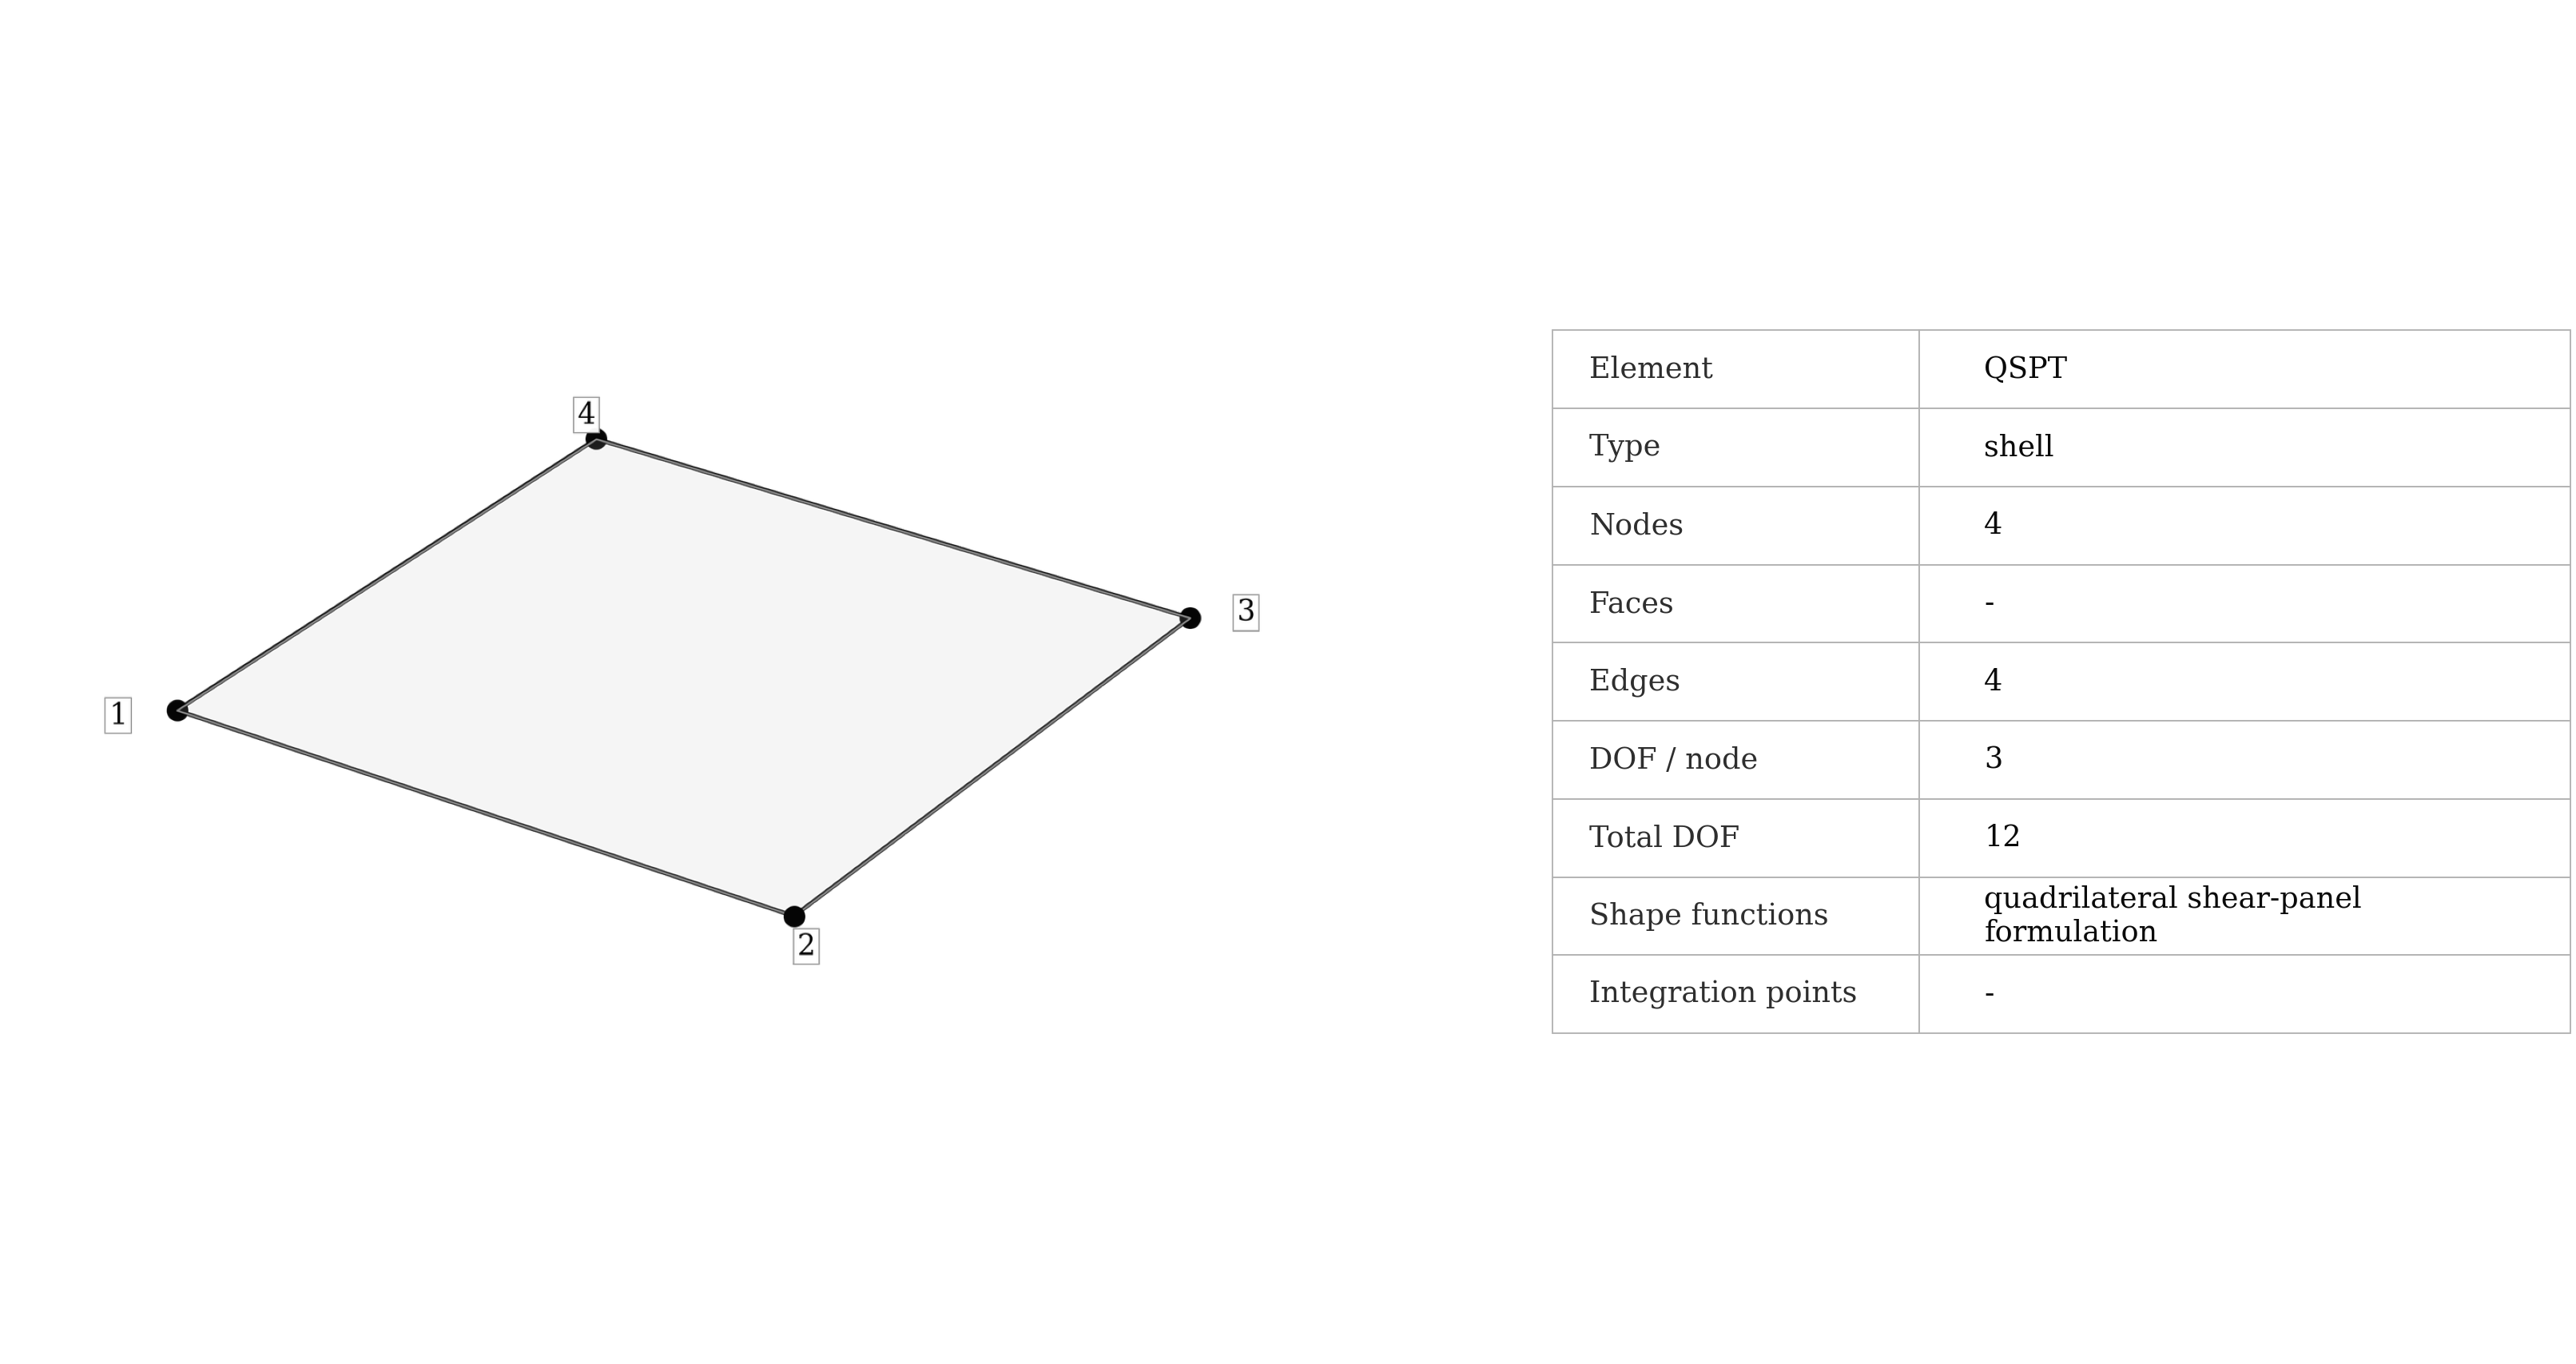
\includegraphics[width=0.78\linewidth]{pages/figures/element_schematics/qspt_schematic.png}
    \caption{\val{QSPT} shear-panel element.}
\end{figure}

\begin{syntax}
*ELEMENT, TYPE=QSPT, ELSET=<set>
<id>, <n1>, <n2>, <n3>, <n4>
\end{syntax}

\val{QSPT} is a specialized four-node quadrilateral panel element developed for shear-flow-oriented structural idealizations. It is intended for simplified panel models where the principal purpose of the element is to transfer in-plane shear rather than reproduce the complete behaviour of a general shell.

Typical applications are preliminary thin-walled structures, webs, aircraft-style shear panels, and reduced-order structural models in which panel shear flow is the primary quantity of interest. In such models \val{QSPT} can provide a compact load-path representation without introducing a complete shell formulation for every panel.

\val{QSPT} is not a general replacement for \val{MITC4FRT} despite sharing a four-node quadrilateral topology. It does not provide the bending stiffness, local shell curvature, full shell resultants, or detailed top/bottom stresses of a shell formulation.

\clearpage
\subsubsection{Beam and truss elements}

Line elements idealize slender three-dimensional members by describing the cross-section through section properties instead of meshing it explicitly. This can reduce the number of degrees of freedom by orders of magnitude compared with shell or solid modelling. The trade-off is that local three-dimensional connection behaviour, detailed cross-section distortion, holes, welds, and local stress concentrations are not resolved.

\clearpage
\paragraph{\val{B31}: 2-node geometrically exact 3D beam}

\begin{syntax}
*ELEMENT, TYPE=B31, ELSET=<set>
<id>, <n1>, <n2>
\end{syntax}

\val{B31} is a two-node shear-flexible spatial beam with three translational and three rotational degrees of freedom per node. The rotational degrees of freedom use FEMaster's total global axis--angle convention. The element evaluates finite rotations on \(SO(3)\), interpolates the relative nodal rotation objectively along the shortest rotation path, and carries the six generalized section strains
\[
[\varepsilon_x,\gamma_y,\gamma_z,\kappa_x,\kappa_y,\kappa_z]^T .
\]

The formulation uses the two end points as order-one Gauss--Lobatto integration points. Axial, transverse-shear, torsional and bending stiffnesses are obtained from the assigned isotropic material and \cmd{PROFILE}. The profile values \(A_{sy}\) and \(A_{sz}\) define the effective shear areas; if they are omitted, both default to \(5A/6\).

Finite section offsets are part of the beam kinematics. With \(SP\) the shear point, \(SMP\) the section material/centroid point and \(REF\) the nodal reference line, the stored profile data define
\[
SP-SMP=(0,e_y,e_z),\qquad
REF-SMP=(0,\mathrm{ref}_y,\mathrm{ref}_z).
\]
The vector from the nodal reference line to the shear point is therefore rotated with the current section orientation. The \(SP-SMP\) eccentricity also enters the sectional constitutive matrix so axial/bending coupling is represented without applying a small-rotation offset matrix after assembly.

For nonlinear static analysis the internal force and the complete tangent are evaluated at the supplied base state. A superposed finite rigid-body translation and rotation therefore produces zero generalized strain. Linear static, eigenfrequency, harmonic and buckling operators use the same B31 reference tangent and mass/geometric operators. The current mass operator is the order-one collocated sectional mass matrix including reference-line eccentricity.

The relative rotation between the two B31 nodes must remain below 180 degrees so the shortest \(SO(3)\) interpolation branch is unique. Large overall rigid-body rotations are not restricted by this condition; it applies only to the relative nodal rotation within one element.

\clearpage
\paragraph{\val{B33}: 3D beam element}

\begin{figure}[H]
    \centering
    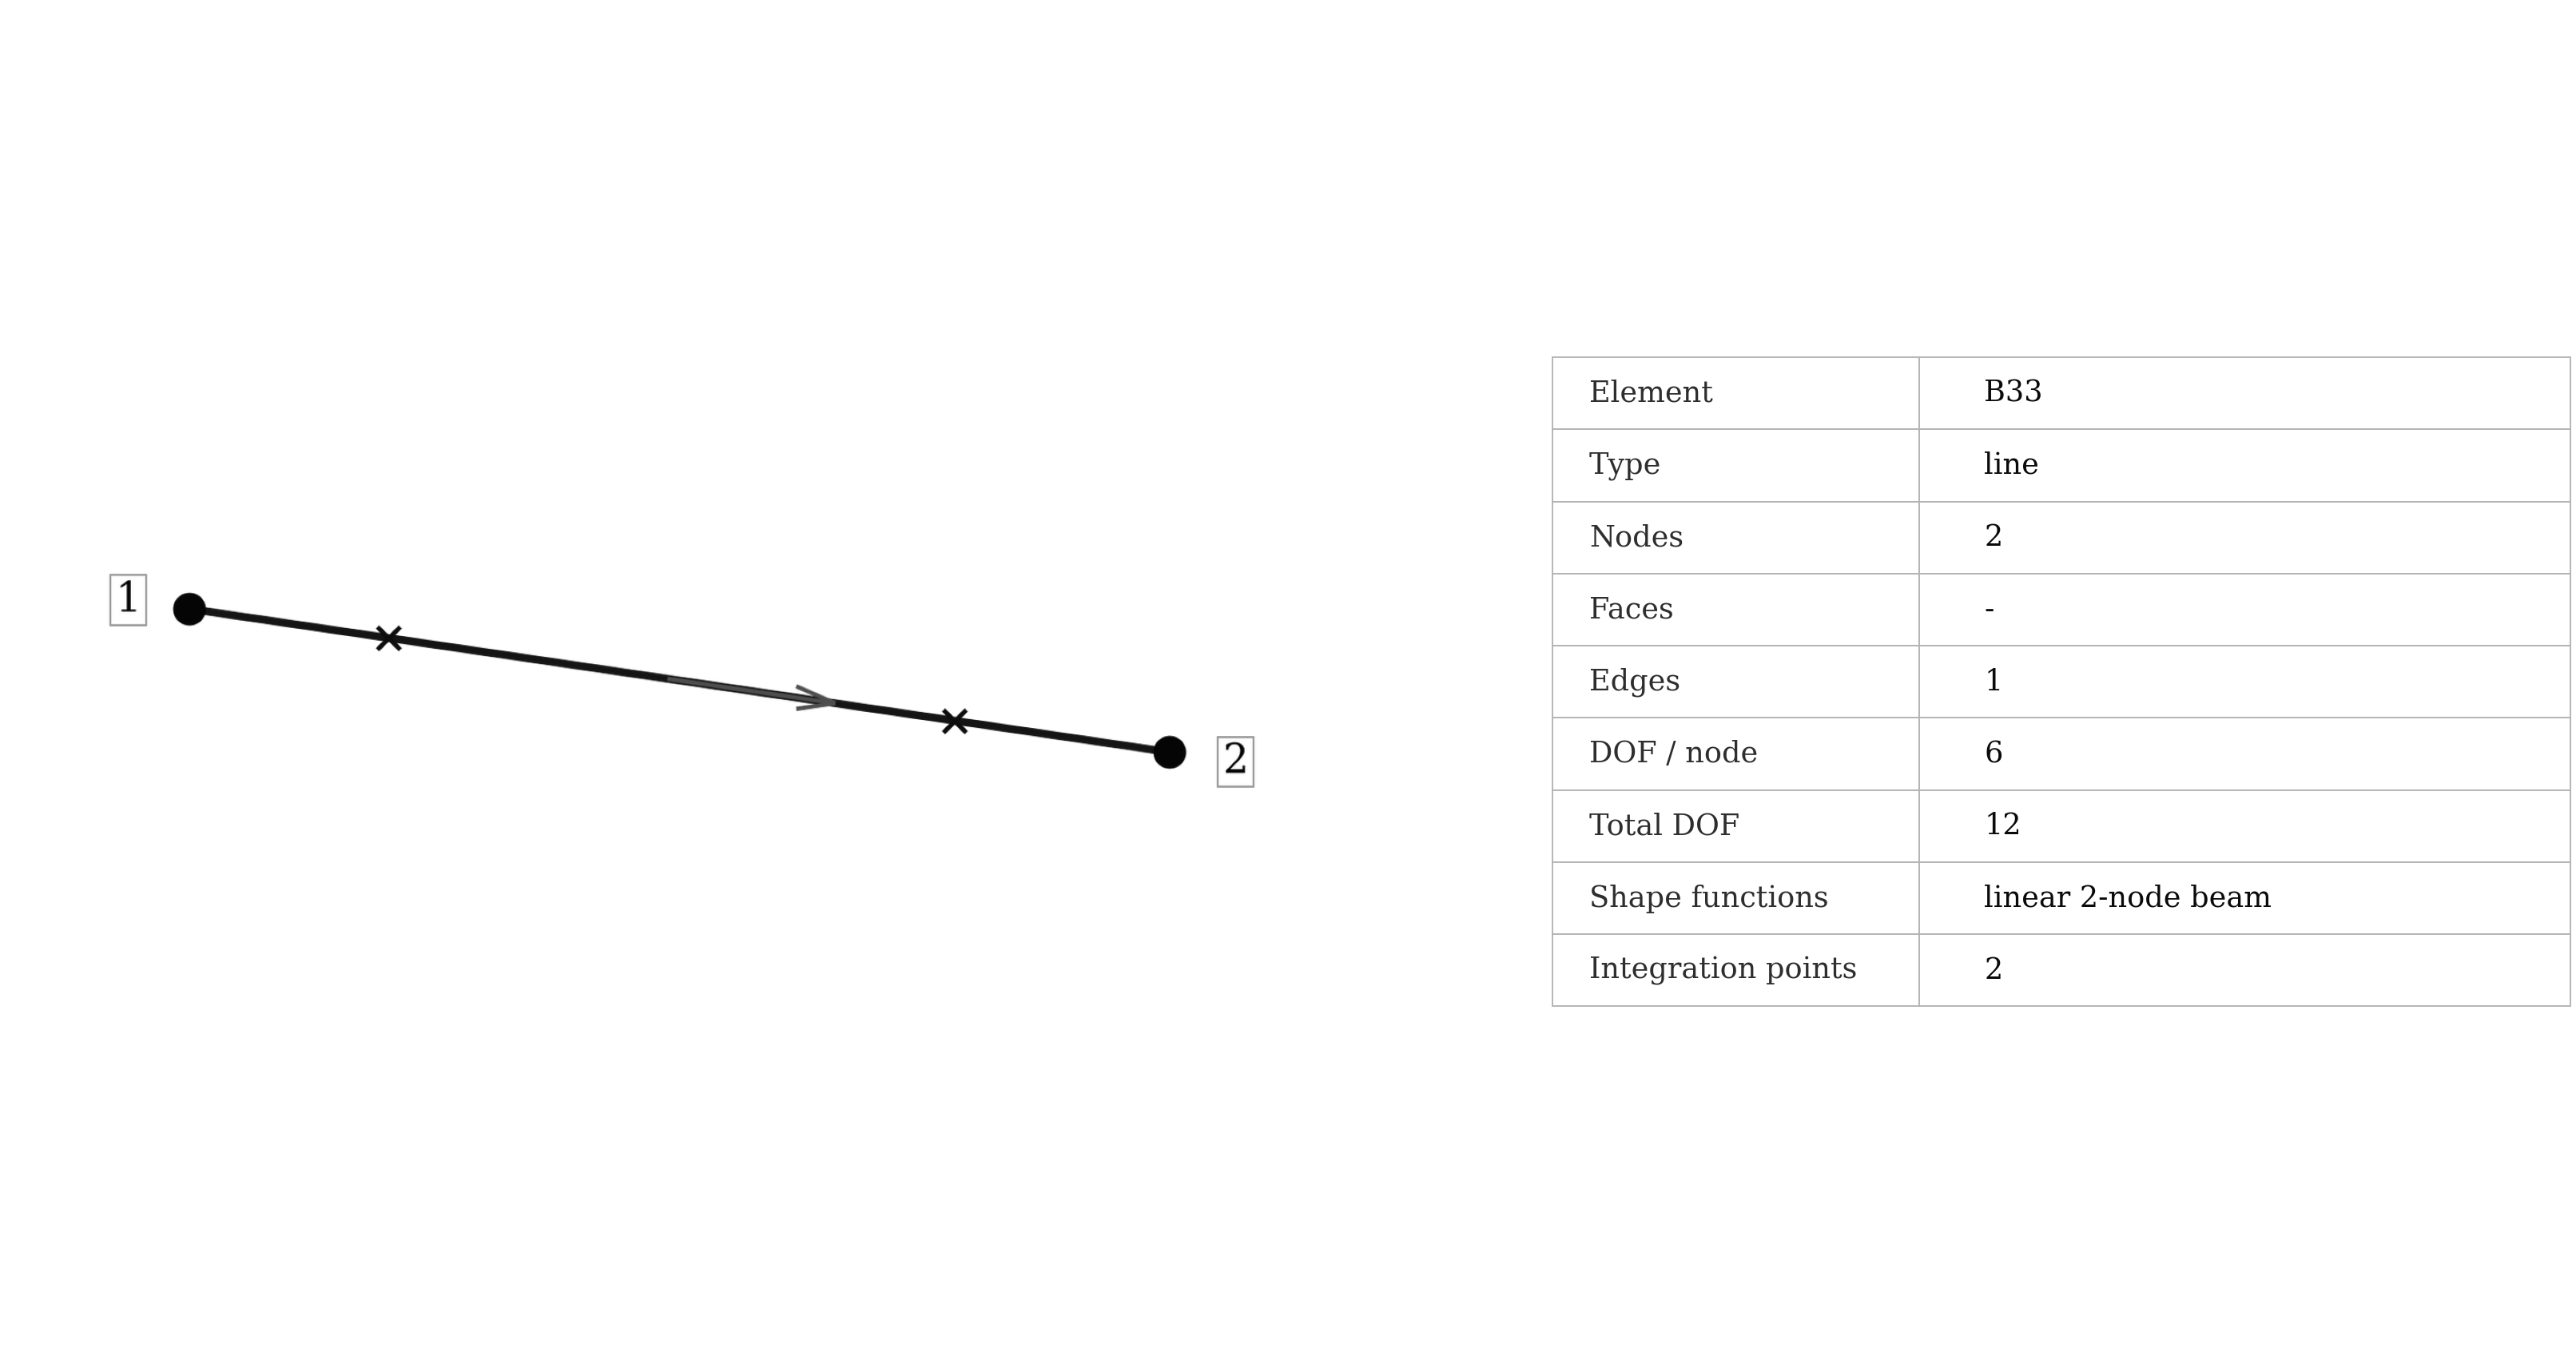
\includegraphics[width=0.70\linewidth]{pages/figures/element_schematics/b33_schematic.png}
    \caption{\val{B33} beam element.}
\end{figure}

\begin{syntax}
*ELEMENT, TYPE=B33, ELSET=<set>
<id>, <n1>, <n2>
\end{syntax}

\val{B33} is a two-node three-dimensional beam element with translational and rotational nodal degrees of freedom. It represents axial deformation, bending, torsion, and the section response defined by \cmd{BEAM SECTION} and the referenced \cmd{PROFILE}.

The current \cmd{ELEMENT} syntax uses exactly two connectivity nodes for \val{B33}. Beam cross-section orientation is supplied by the orientation vector in \cmd{BEAM SECTION}; an additional orientation node is not part of the current connectivity grammar.

Beam elements represent slender frames, stiffeners, spars, ribs, idealized support members, and other structures through Section forces and global deformation. They include axial area, bending inertias, torsional stiffness, product of inertia, Section offsets, and reference-line offsets without meshing the full cross-section.

The beam idealization does not resolve local connection stresses, bolt or weld geometry, detailed cross-section deformation, or three-dimensional load introduction. Those effects require a corresponding shell or solid representation. The beam local axes determine the interpretation of bending moments, section forces, and profile properties.

The Abaqus-compatible \val{B33} name uses the same two-node connectivity.

\clearpage
\paragraph{\val{T3}: 2-node truss element}

\begin{figure}[H]
    \centering
    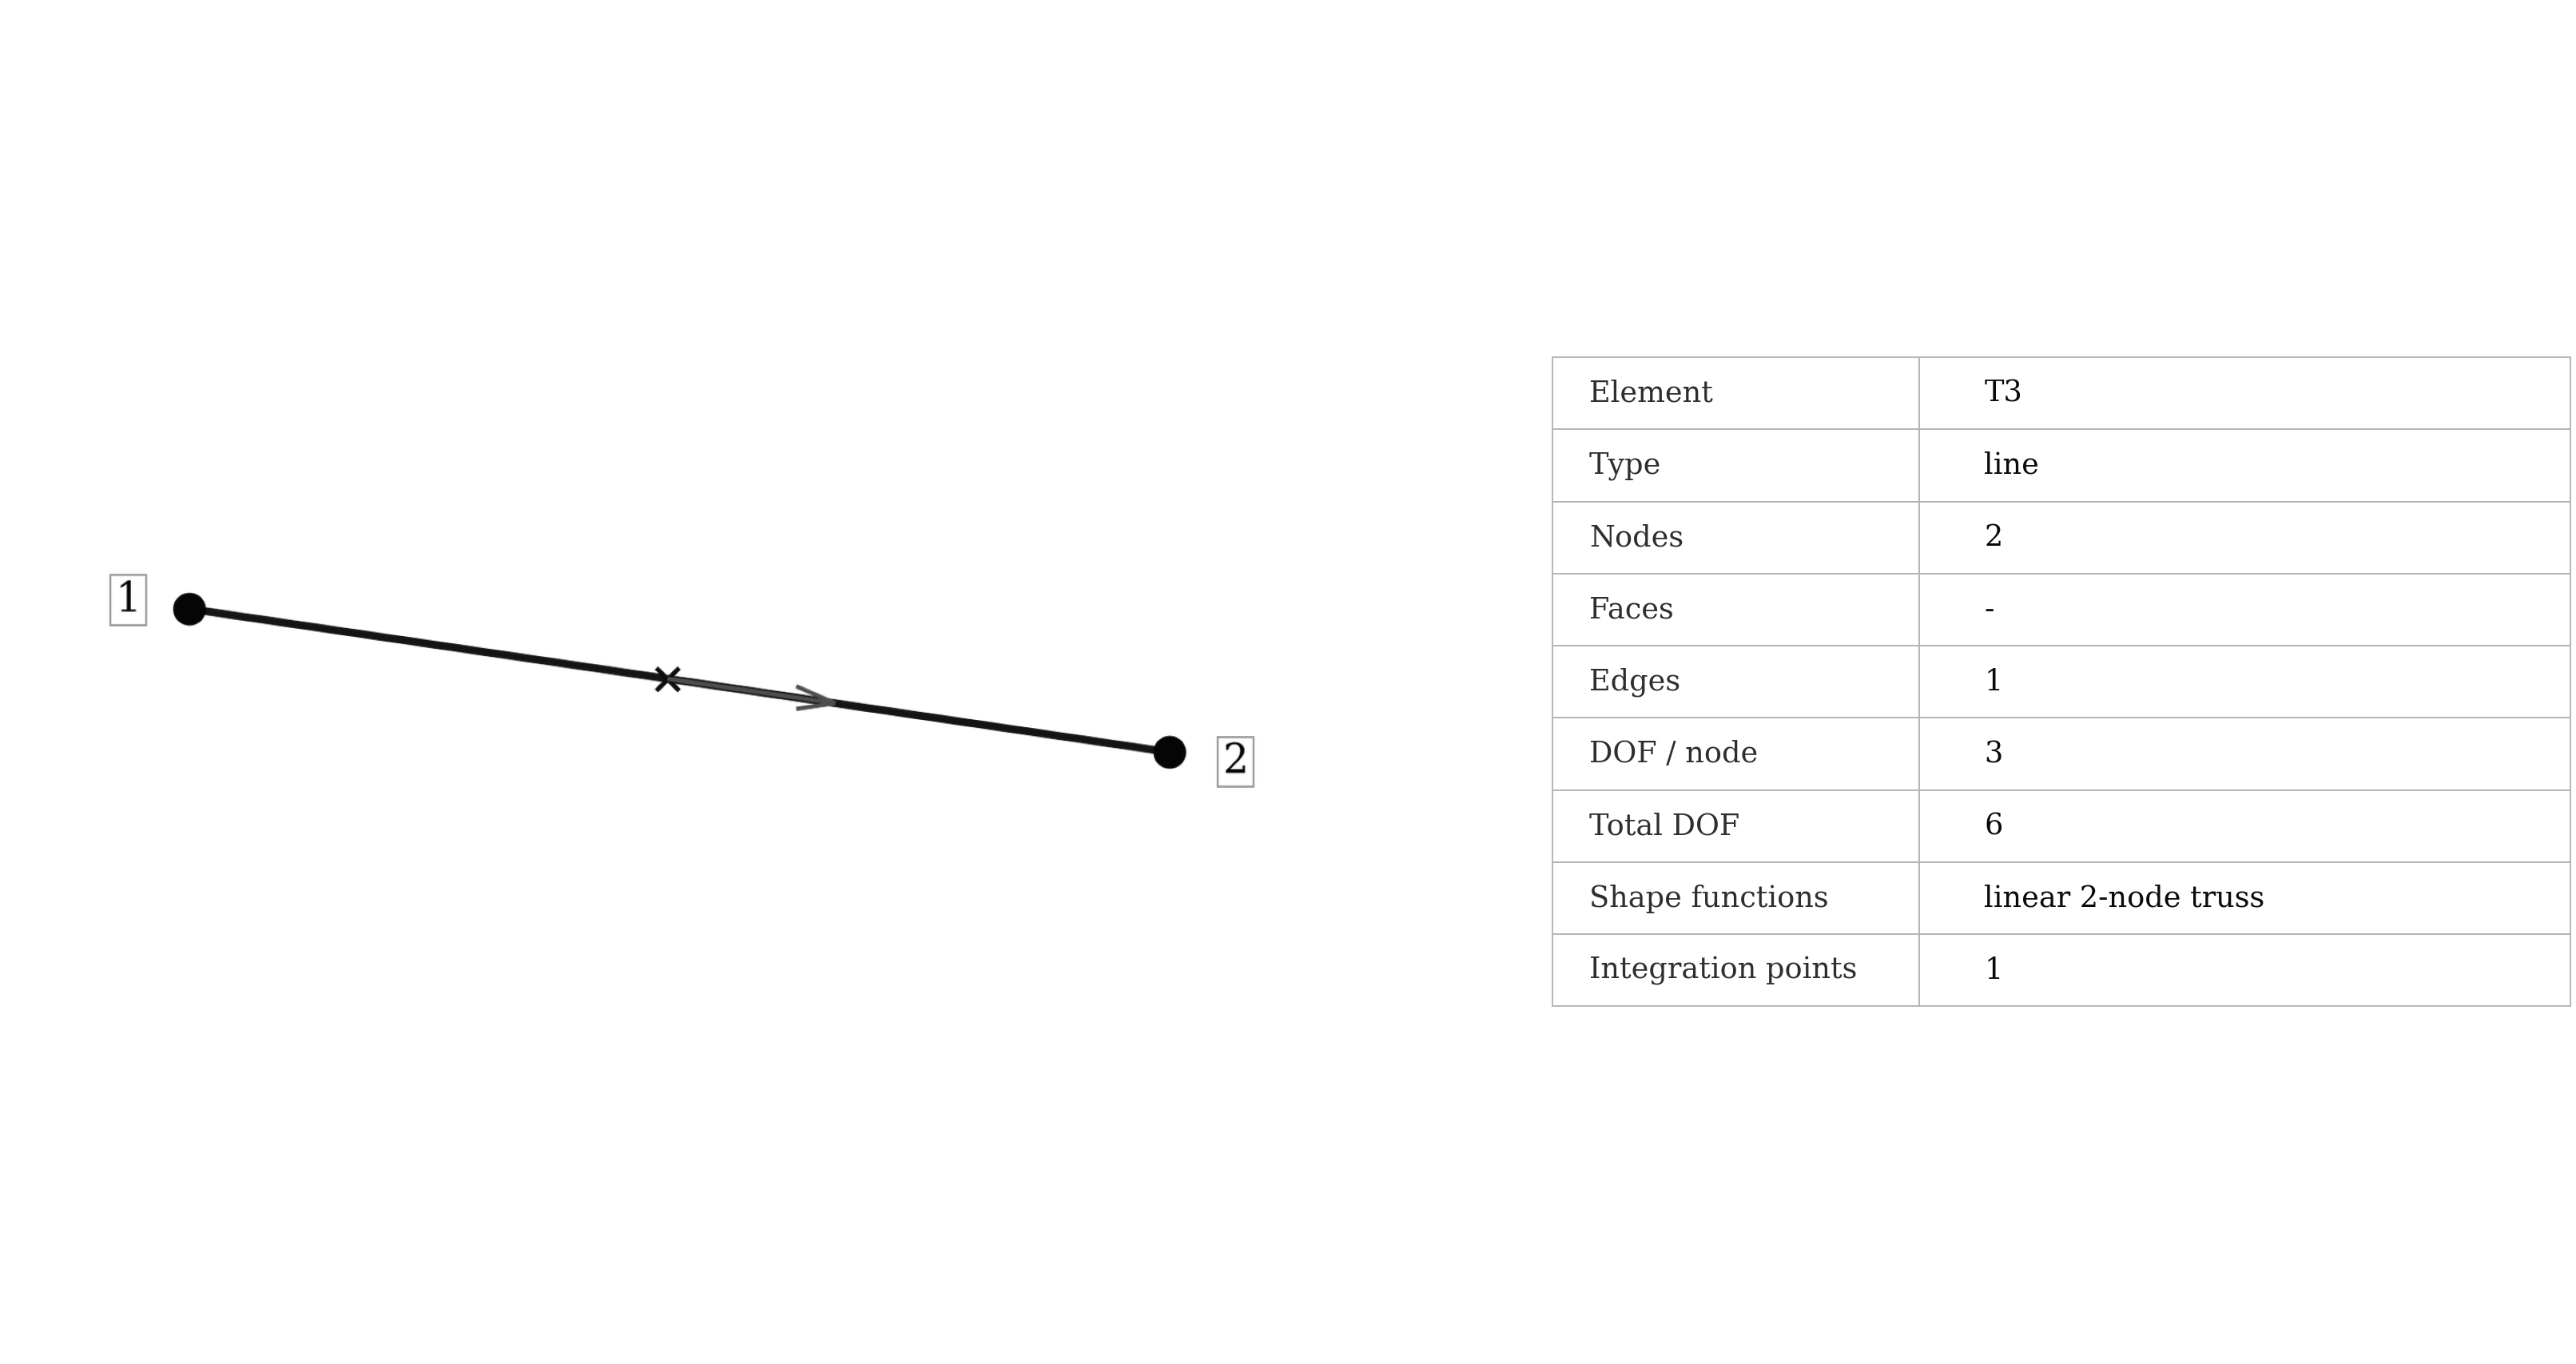
\includegraphics[width=0.68\linewidth]{pages/figures/element_schematics/t3_schematic.png}
    \caption{\val{T3} truss element.}
\end{figure}

\begin{syntax}
*ELEMENT, TYPE=T3, ELSET=<set>
<id>, <n1>, <n2>
\end{syntax}

\val{T3} is a two-node truss element. It carries axial force along its current line direction and uses translational nodal degrees of freedom. The material and cross-sectional area are assigned by \cmd{TRUSS SECTION}.

The element represents pin-jointed members, rods, braces, links, and other components whose structural action is axial tension or compression. Its mechanical quantities are axial force, axial strain, and axial stress.

The limitations are deliberate. \val{T3} has no bending stiffness, no torsional stiffness, and no rotational continuity. It cannot model fixed-end moments, eccentric frame action, or transverse stiffness of a physical beam; those behaviours require \val{B33} or a shell/solid representation.

The Abaqus-compatible name \val{T3D2} selects the same FEMaster truss formulation as \val{T3}.

\begin{inputdeck}[Abaqus-compatible alternative]
*ELEMENT, TYPE=T3D2, ELSET=BARS
10, 1, 2
\end{inputdeck}

\clearpage
\subsubsection{Point elements}

Point elements are zero-dimensional structural elements attached to a single node. They preserve element identity and ELSET membership while their physical contribution is supplied by an assigned point-mass section rather than by continuum geometry or a material law. The unified input language accepts three regular one-node types: \val{MASS}, \val{ROTARYI}, and \val{SPRING1}. Internally all three use the same \texttt{PointElement}; the corresponding property keyword determines which generalized diagonal coefficient is populated.

A point element without an assigned point property is intentionally inert. It has zero stiffness, zero mass, no stress or strain state, and activates no degrees of freedom. Property definitions are documented in Section~\ref{sec:sections}; this section focuses on the element topology and kinematic role.

\clearpage
\paragraph{\val{MASS}: 1-node concentrated-mass element}

\begin{syntax}
*ELEMENT, TYPE=MASS, ELSET=<set>
<id>, <node>
*MASS, ELSET=<set>
<mass>
\end{syntax}

\val{MASS} is an Abaqus-compatible one-node point element. The \cmd{ELEMENT} record creates only topology: an element ID, one connected node, and normal ELSET membership. The scalar physical mass is assigned separately by \cmd{MASS, ELSET=...}.

For the supported isotropic property, the element mass matrix is
\[
M_e=\operatorname{diag}(m,m,m,0,0,0),
\]
so a positive mass activates the three translational components at the connected node. Several \val{MASS} elements may reference the same node; each represents an independent concentrated contribution and the assembled mass is additive.

The point element has zero geometric volume, but its density-scaled field integration interprets \(m\) as the complete concentrated mass measure. Consequently, a regular \val{MASS} element contributes to the global mass matrix, eigenfrequency and transient analyses, inertia relief, and element-targeted mass-proportional body or inertial loads. The Abaqus-compatible \cmd{DLOAD} with \val{GRAV} produces the concentrated force \(m\boldsymbol a\) when the selected element region contains the point element. FEMaster-specific \cmd{VLOAD} instead denotes force density and does not load this zero-volume point element.

Part-local \val{MASS} elements and their \cmd{MASS} property assignments are copied to every Instance during model compilation. An assembly-level \cmd{MASS} assignment instead targets compiled point elements through an assembly ELSET.

\textbf{Alternative:} For concentrated mass that does not require
an explicit element ID or ELSET membership, the FEMaster-specific
\cmd{POINTMASS} keyword assigns a mass directly to an NSET:

\begin{inputdeck}[FEMaster-specific alternative]
*POINTMASS, NSET=PAYLOAD_NODES
0.025
\end{inputdeck}

This creates auxiliary point elements during model compilation.
The specified value is applied independently to each node in the
set; load selection and element-set behavior differ from a regular
\val{MASS} element. See Section~\ref{sec:sections}.

\clearpage
\paragraph{\val{ROTARYI}: 1-node rotary-inertia element}

\begin{syntax}
*ELEMENT, TYPE=ROTARYI, ELSET=<set>
<id>, <node>
*ROTARY INERTIA, ELSET=<set>
<I11>, <I22>, <I33>, <I12>, <I13>, <I23>
\end{syntax}

\val{ROTARYI} is the rotational-inertia counterpart of \val{MASS}. Its one-node topology is identical, but the property acts on the rotational degrees of freedom. FEMaster's supported diagonal mapping produces
\[
M_e=\operatorname{diag}(0,0,0,I_{11},I_{22},I_{33}).
\]
Each nonzero diagonal inertia activates its corresponding nodal rotation.

Abaqus permits the full symmetric rotary-inertia tensor. The current FEMaster point section stores only the diagonal moments, so the data positions \(I_{12}\), \(I_{13}\), and \(I_{23}\) are accepted only when zero. Orientation-dependent rotary inertia is likewise outside the current mapping.

A \val{ROTARYI} element can share its connected node with a \val{MASS} element. This is the regular element-based way to represent translational mass and rotary inertia at the same physical point while preserving the Abaqus separation between the two element families.

\clearpage
\paragraph{\val{SPRING1}: 1-node point-to-ground spring}

\begin{syntax}
*ELEMENT, TYPE=SPRING1, ELSET=<set>
<id>, <node>
*SPRING, ELSET=<set>
<dof>
<stiffness>
\end{syntax}

\val{SPRING1} is a one-node spring between the connected node and ground. The first \cmd{SPRING} data line selects the generalized nodal direction; the second gives the constant linear stiffness. Degrees of freedom 1--3 act on translations and degrees of freedom 4--6 act on rotations.

For one selected direction the point-element stiffness matrix contains exactly one nonzero diagonal entry. Translational DOFs therefore represent ordinary point-to-ground springs, whereas rotational DOFs represent torsional point-to-ground springs. Multiple independent directions are represented by multiple \val{SPRING1} elements, which may all reference the same node.

The current mapping is deliberately narrower than the complete Abaqus spring family. It supports only real, constant, linear \val{SPRING1} behavior in the global nodal system. \val{SPRING2}, \val{SPRINGA}, local orientations, nonlinear force--displacement curves, frequency or field dependence, and complex stiffness are not mapped.

The FEMaster-specific \cmd{POINTMASS} keyword provides an alternative NSET-based convenience syntax when mass, rotary inertia, and several diagonal translational or rotational springs should be combined directly on the same target nodes. It creates auxiliary post-compile point elements rather than regular ELSET members.

\addtocontents{toc}{\protect\setcounter{tocdepth}{3}}

